% mnras_template.tex 
%
% LaTeX template for creating an MNRAS paper
%
% v3.0 released 14 May 2015
% (version numbers match those of mnras.cls)
%
% Copyright (C) Royal Astronomical Society 2015
% Authors:
% Keith T. Smith (Royal Astronomical Society)

% Change log
%
% v3.0 May 2015
%    Renamed to match the new package name
%    Version number matches mnras.cls
%    A few minor tweaksto wording
% v1.0 September 2013
%    Beta testing only - never publicly released
%    First version: a simple (ish) template for creating an MNRAS paper

%%%%%%%%%%%%%%%%%%%%%%%%%%%%%%%%%%%%%%%%%%%%%%%%%%
% Basic setup. Most papers should leave these options alone.
\documentclass[fleqn,usenatbib, useAMS, a4paper]{mnras}


\usepackage{savesym}
\savesymbol{tablenum}
\usepackage{siunitx}
\restoresymbol{SIX}{tablenum}


% MNRAS is set in Times font. If you don't have this installed (most LaTeX
% installations will e fine) or prefer the old Computer Modern fonts, comment
% out the following line
\usepackage{newtxtext}
\usepackage[varg,varvw,smallerops]{newtxmath}
% Depending on your LaTeX fonts installation, you might get better results with one of these:
%\usepackage{mathptmx}
%\usepackage{txfonts}

% Use vector fonts, so it zooms properly in on-screen viewing software
% Don't change these lines unless you know what you are doing
\usepackage[T1]{fontenc}
\usepackage{ae,aecompl}


%%%%% AUTHORS - PLACE YOUR OWN PACKAGES HERE %%%%%

% Only include extra packages if you really need them. Common packages are:
\usepackage{graphicx}	% Including figure files
\let\Bbbk\relax
\usepackage{amsmath}	% Advanced maths commands
\usepackage{amssymb}	% Extra maths symbols
\usepackage{multicol}
\usepackage{enumerate}          % Better lists
\usepackage{xcolor}

%% Package set-up
\usepackage{booktabs}
\usepackage{array}   % for \newcolumntype macro
\newcolumntype{L}{>{$}l<{$}} % math-mode version of lrc column types
\newcolumntype{R}{>{$}r<{$}} 
\newcolumntype{C}{>{$}c<{$}}

% Use more muted colors for links
\hypersetup{colorlinks=True, linkcolor=blue!50!black, citecolor=black,
  urlcolor=blue!50!black}

% Tweaks to siunitx configuration
\sisetup{
  % explicit""+" is useful for velocities
  retain-explicit-plus = true,
  % prefer 10^6 over 1 x 10^6
  retain-unity-mantissa = false,
  % Use x +/- e instead of x(e)  
  separate-uncertainty = true,
  % Make sure to pick up bold font when used in section heading for instance
  detect-weight = true,
}

%%%%%%%%%%%%%%%%%%%%%%%%%%%%%%%%%%%%%%%%%%%%%%%%%%

%%%%% AUTHORS - PLACE YOUR OWN COMMANDS HERE %%%%%

% Please keep new commands to a minimum, and use \newcommand not \def to avoid
% overwriting existing commands. Example:
%\newcommand{\pcm}{\,cm$^{-2}$}	% per cm-squared

% A better \ion command that works in more circumstances
\newcommand\ION[2]{#1\,\scalebox{0.9}[0.8]{\uppercase{#2}}}

\newcounter{ionstage}
\renewcommand{\ion}[2]{\setcounter{ionstage}{#2}% 
  \ensuremath{\mathrm{#1\,\scriptstyle\Roman{ionstage}}}}
  
\newcommand\hii{\ion{H}{2}}
\newcommand\pos{\ensuremath{_{\mathrm{pos}}}}
\newcommand\los{\ensuremath{_{\mathrm{los}}}}
\newcommand\noise{\ensuremath{_{\text{noise}}}}
\newcommand\obs{\ensuremath{_{\mathrm{obs}}}}
\newcommand\model{\ensuremath{_{\mathrm{mod}}}}
\newcommand\halpha{H${\alpha}$}
\newcommand\n{[\ion{N}{II}]$\lambda$6584}
\newcommand\oi{[\ion{O}{III}]$\lambda$5007}
\newcommand\s{[\ion{S}{II}]$\lambda$6737}
\newcommand\kms{$^{-1}$}

\newcommand\ha{\ensuremath{\text{H}\alpha}}
\newcommand\Wav[1]{\ensuremath{\lambda #1}}
% Chemical formulae
\newcommand*\chem[1]{\ensuremath{\mathrm{#1}}}
\newcommand\csound{\ensuremath{c_{\text{s}}}}
\newcommand\FNa{\textsuperscript{a}}

%%%%%%%%%%%%%%%%%%%%%%%%%%%%%%%%%%%%%%%%%%%%%%%%%%

%%%%%%%%%%%%%%%%%%% TITLE PAGE %%%%%%%%%%%%%%%%%%%

% Title of the paper, and the short title which is used in the headers.
% Keep the title short and informative.
\title[Turbulence in H II regions]{Turbulence in compact to giant HII regions}

% The list of authors, and the short list which is used in the headers.
% If you need two or more lines of authors, add an extra line using \newauthor
\author[J. García Vázquez et al.]{
J. García Vázquez,$^{1}$\thanks{E-mail: jgarciav1600@alumno.ipn.mx}
J. Zsargo,$^{1}$
and W. J. Henney$^{2}$
%and H. O. Castañeda$^{1}$
\\
% List of institutions
$^{1}$Escuela Superior de Física y Matemáticas, Instituto Politécnico Nacional, Ciudad de México, México.\\
$^{2}$Instituto de Radioastronomía y Astrofísica, Universidad Nacional Autonoma de México, Apartado postal 3-72, 58090 Morelia, Michoacán, Mexico\\
}

% These dates will be filled out by the publisher
\date{Accepted XXX. Received YYY; in original form ZZZ}

% Enter the current year, for the copyright statements etc.
\pubyear{2021}

% Don't change these lines
\begin{document}
\label{firstpage}
\pagerange{\pageref{firstpage}--\pageref{lastpage}}
\maketitle

% Abstract of the paper
\begin{abstract}
  Fluctuations of centroid velocities on the plane of the sky derived from spectroscopic observations are a powerful tool for studying the turbulent dynamics of emission line regions.
  With the aim to characterize these velocities fluctuations we conduct a statistical analysis on a diverse sample of 9 \hii{} regions that spans more than two orders of magnitude in size and luminosity located in the Milky Way and other Local Group galaxies.
  We determine the second-order structure function of the centroid velocity two-dimensional map of the \halpha\ emission line.
  We also proposed a heuristic model for the structure function which takes into account observational constraints like the seeing (\(s_0\)), instrumental noise (\(B_{\text{noise}}\)) and size of the field of view (\(L_{\text{box}}\)), and the turbulent velocity field parameters like the velocity dispersion of the centroid velocity (\(\sigma\pos\)), the autocorrelation length (\(r_0\)) and a power-law index (\(m\)).
  The observational structure function is fitted using our heuristic model in a non-linear regression analysis which allow us to derive the parameters previously mentioned  with their respective confidence intervals.
  Our results are: \(\num{0.2} < s_0 \text{(FWHM)} < \SI{3.0}{arcsec}\), \(\num{0.003} < B_{\text{noise}} < \SI{6.0}{km^{-2}.s^{-2}}\),  \(\num{3} < \sigma\pos < \SI{19}{km.s^{-1}}\), \(\num{0.07} < r_0 < \SI{12}{pc}\) and \(\num{0.7}< m < \num{1.5}\). 
  The derived parameters are used to determine scaling relations between the physical properties of the regions like \halpha\ luminosity (\(L(H_{\alpha})\)), diamater (\(D\)) and the mean non-thermal linewidth (\(\langle \sigma_{los} \rangle\)).
  We find that these relations are \(\sigma\pos \propto L(H_{\alpha})^{0.28 \pm 0.10}\) and \(r_0 \propto D^{0.95 \pm 0.32}\), and that the \(\sigma\pos\) and \(\langle \sigma_{los} \rangle\), values increase following a linear monotonically relation.
  Since the derived  scale-relations are within the uncertainty of previous investigations we conclude that the parameters obtained from our proposed model represents true kinematic properties of each region.
  The methodology we present guarantees consistency for comparison between the galactic and giant HII regions. 
%  The second-order structure function has proved to be a useful tool to determine the existence of the correlations between random velocities and distance across the \hii{} regions.

  
  
\end{abstract}

% Select between one and six entries from the list of approved keywords.
% Don't make up new ones.
\begin{keywords}
turbulence -- instrumentation: spectrographs -- ISM: HII regions, kinematics and dynamics
\end{keywords}


\definecolor{WillCommentColor}{rgb}{0.6,0.11,0.4}
\newcommand\WILL[1]{\textbf{\color{WillCommentColor}#1}}
%%%%%%%%%%%%%%%%%%%%%%%%%%%%%%%%%%%%%%%%%%%%%%%%%%

%%%%%%%%%%%%%%%%% BODY OF PAPER %%%%%%%%%%%%%%%%%%

\section{Introduction}


%% Will version 2021-12-07 of Intro first para (what we are studying)
Photoionized regions around high-mass stars (\hii{} regions)
show highly vigorous dynamics
as a result of the star formation process and the energy and momentum
injected by the newly-formed stars.
Rather than manifesting a simple pattern such as expansion, infall, or rotation,
the motions are frequently disordered or ``turbulent''
and must be characterised by statistical techniques.
In relatively low luminosity regions, such as the nearby Orion Nebula,
the disordered motions are approximately transonic,
with typical velocities of order \num{5} to \SI{10}{km.s^{-1}}
\citep{castaneda1988, Garcia-Diaz:2008a}.
In larger, higher luminosity regions,
such as 30~Doradus in the Large Magellanic Cloud,
the velocities are significantly supersonic,
of order \SI{30}{km.s^{-1}} \citep{Torres-Flores:2013t, Castro:2018a}.
The same tendency of increasing velocity dispersion (\(\sigma\))
and luminosity (\(L\))
continues up to the scale of entire galaxies
with an approximate relation \(L \propto \sigma^\alpha\) that spans
more than 5 orders of magnitude in luminosity
with a  power-law index \(\alpha = 3\) to~\(7\)
\citep{terlevich1981, Rozas:2006b, Chavez:2014a, Moiseev:2015a}.
However, it is not known whether a single physical mechanism
underlies this relationship at all scales.
The relative importance of gravity and the various stellar feedback mechanisms
(heating, direct radiation pressure, stellar winds, cluster winds)
are unclear in many cases and are frequently disputed \citep{Krumholz:2016a, Melnick:2021x}.

%% Will version 2021-12-07 of Intro second para (how we are studying it)
One of the simplest ways to measure the velocity dispersion of an \hii{} region
is to use the Doppler width of a strong emission line, such as the
optical hydrogen recombination line \ha{} \Wav{6563}
\citetext{e.g., \citealp{1986ApJ...300..624R}}.
We will use \(\sigma\los\) to denote
the root-mean-square (RMS) line-of-sight velocity dispersion determined in this way.
Unfortunately, there are many processes that contribute to this width
in addition to the line-of-sight turbulent velocity fluctuations,
such as thermal and fine-structure broadening, instrumental broadening,
dust scattering, 
and large-scale expansion
\citetext{see \citealp{Rozas:2006b} and \citealp{Garcia-Diaz:2008a}
  for detailed discussion}.
All except the last of these can in principal be approximately corrected for,
which is a reasonable strategy to apply in the case of high-luminosity regions
where the turbulent width is expected to be larger than the correction terms.
However, for lower luminosity regions the turbulent velocities are much smaller,
which limits the accuracy of such a correction process
\citetext{see section 3.4 of \citealp{arthur2016turbulence}}. 

An alternative way to study turbulent motions is to measure
the fluctuations on the plane of the sky of the velocity centroids of an emission line
\citep{von1951methode}.
We will denote the RMS magnitude of these fluctuations by \(\sigma\pos\).
In addition to being unaffected by the various nuisance broadening mechanisms
discussed in the previous paragraph,
this also offers the opportunity to study the spatial scale of the fluctuations
by measuring average velocity differences as a function of
the angular separation between two points.
Different mathematical tools can be used to study these spatial fluctuations,
such as the autocorrelation function \citep{lagrois2011}
and \(\Delta\)-variance \citep{Ossenkopf:2006a}.
In this work, we will concentrate on the second order structure function,
\(B(r)\) (see section \ref{sec:second-order-struct}),
which has been used in many previous studies of velocity fluctuations
in \hii{} regions in our own Galaxy
% Javier cited the wrong Roy & Joncas here - now corrected (should be 1985 not 1986)
% Also, Medina+ 2014  better than Arthur+ 2016
\citep{munch1958internal, castaneda1988, Roy:1985a, 1992ApJ...387..229O, medina2014}
and in external galaxies
\citep{1961MNRAS.122....1F, Medina-Tanco:1997a, lagrois2009multi, lagrois2011, Melnick:2021x}.

% Will's 2021-12-08 new version of Intro para 4: description of our methodology
In this paper,
we employ archival data from a wide variety of integral field and multi-longslit
spectrographic datasets to analyze spatially resolved \ha{} velocity maps for a sample of
nine \hii{} regions (Figure~\ref{fig:hii-regions}),
ranging in size from \SI{0.5}{pc} to \SI{200}{pc}
and in \ha{} luminosity from \SI{e37}{erg.s^{-1}} to  \SI{e39}{erg.s^{-1}}.
The observations and the physical characteristics of our sample
are described in section~\ref{sec:HIIsample}.

We apply a uniform methodology to the analysis of the structure function
by fitting a simple functional form that consists of a power law of slope \(m\)
at small separations,
transitioning to a constant value at separations larger than
an autocorrelation length \(r_0\).
This is described in section~\ref{sec:met}.
We also take into account three observational limitations of the datasets:
the finite angular resolution, \(s_0\) (set by pixel spacing or atmospheric seeing);
the finite map size, \(L_{\text{box}}\);
and a contribution of spatially uncorrelated noise, \(B_0\),
to the observed structure function.
In Appendix~\ref{sec:degr-struct-funct} we use simulated velocity maps to derive
appropriate functional forms for the effects of \(s_0\), \(L_{\text{box}}\) and \(B_0\).
In our fits, we marginalize over these nuisance parameters to obtain robust
credibility limits for the parameters of astrophysical interest:
\(\sigma\pos\), \(r_0\), and \(m\).
The results of these fits are presented in section~\ref{sec:results}.

In section~\ref{sec:discussion} we discuss the relation
of our results to previous studies and the correlations that we find
between the structure function parameters and other properties of
the \hii{} regions in our sample.
%We also discuss the implications of our results for the existence of a
%Kolmogorov-type turbulent energy cascade and the nature of the driving mechanism
%for the velocity fluctuations.
Finally, in section~\ref{sec:conclusions} we present our conclusions.

%% Previous Javier version of final paragraphs of Intro. I think I
%% have incorporated most of this in my own version, but more
%% concisely.  However, I haven't mentioned the projection effects -
%% maybe that would be tetter just in section 3

\section{\boldmath Observations of the \hii{} region sample}
\label{sec:HIIsample}

\begin{figure*}
  \centering
  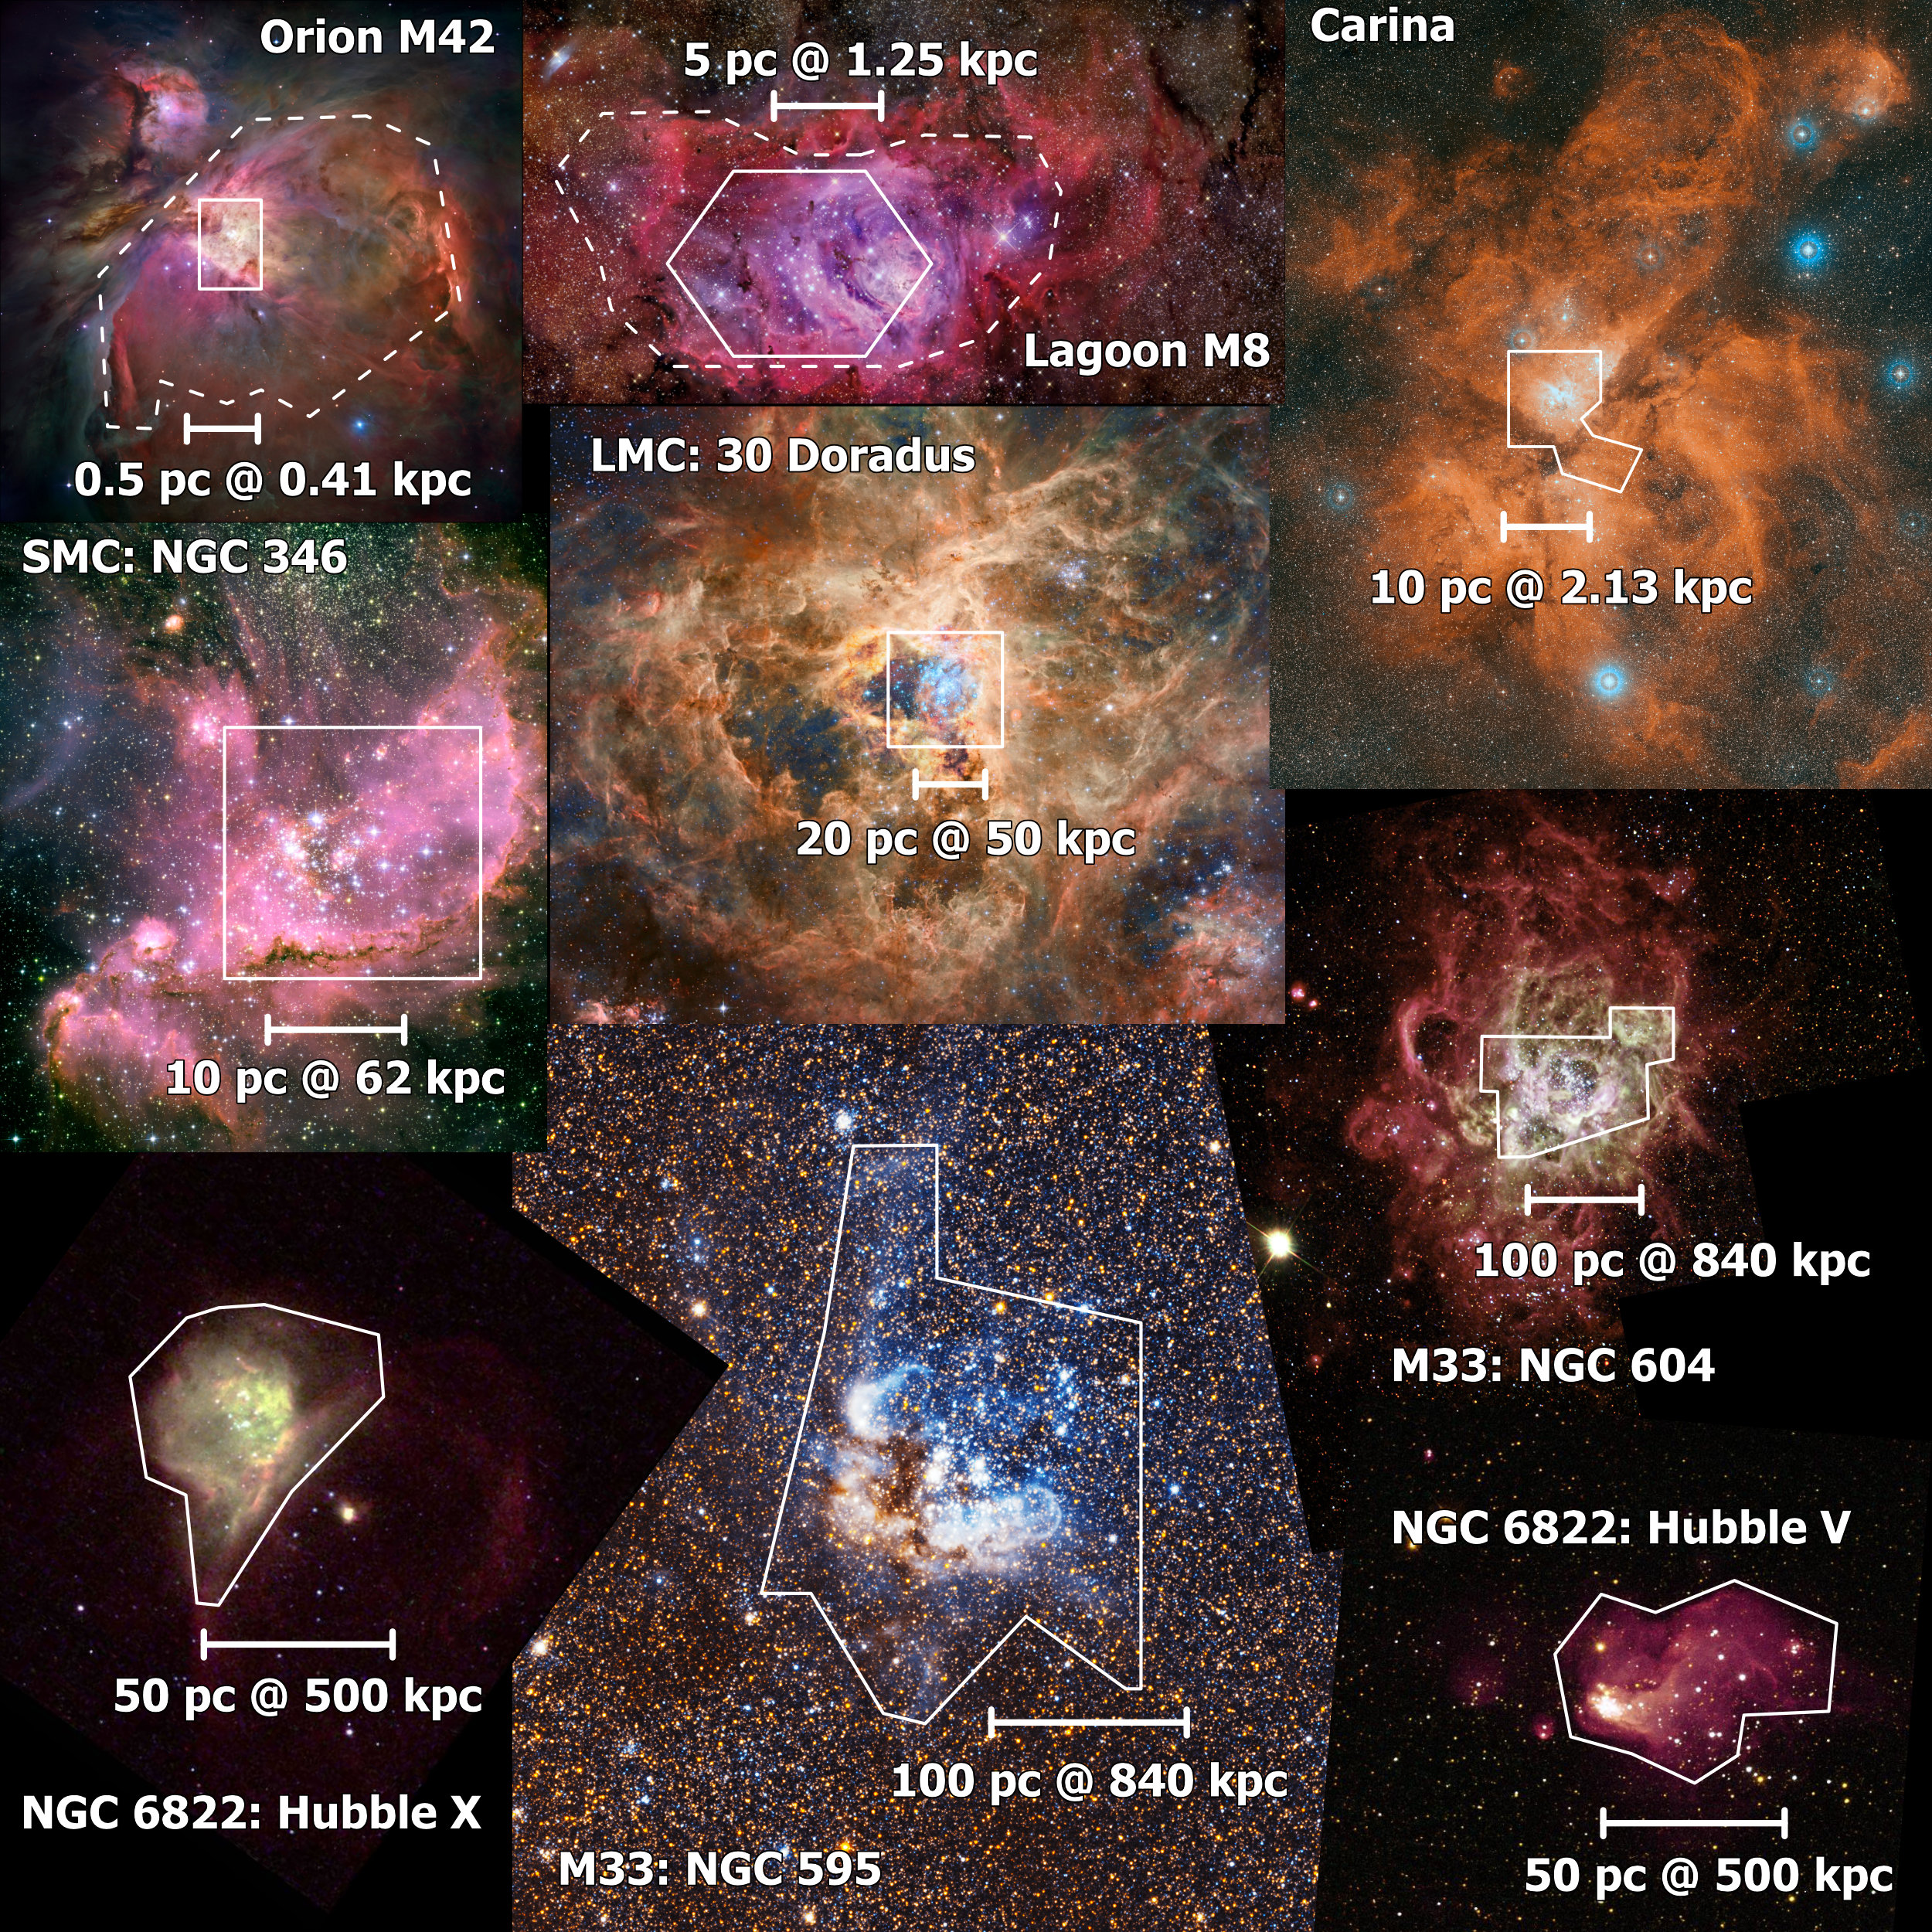
\includegraphics[width=\linewidth]{Figures/hii-region-mosaic}
  \caption{
    The sample of nine \hii{} regions employed in this study,
    arranged from top to bottom in order of distance.
    White shapes show the approximate extents of the
    emission line maps that we use for studying the ionized gas kinematics.
    Scale bars show the equivalent linear length scales at the distance to each region.
    For Orion, two fields are shown: the Extended Orion Nebula,
    sampled at a scale of \SI{0.1}{pc}, and the central Huygens region,
    sampled at a scale of \SI{0.004}{pc}.
    All images are combinations of optical narrow-band and wide-band filters.
    In most cases, red/orange/pink represents \ha{} or other emission lines
    emitted by the ionized gas,
    while blue/white represents continuum starlight from young high-mass stars.
    In some cases, green (for Hubble~X and NGC~604) or blue (for NGC~595)
    represents the [\ion{O}{3}] \Wav{5007} emission line.
    \textit{Image credits as follows.}
    \textbf{Orion Nebula}:
    \textit{HST} Treasury Program on the Orion Nebula Cluster \citep{Robberto:2013a}.
    \textbf{M8 Lagoon}: \href{https://www.cosmotography.com/index.html}{R.~Jay Gabany}.
    \textbf{Carina}: \href{https://www.eso.org/public/images/eso0905b}{
      ESO/Digitized Sky Survey~2, Davide De Martin}.
    \textbf{NGC~346}:
    NASA, ESA and A. Nota (ESA/STScI) \citep{Nota:2006x}.
    \textbf{30 Doradus}:
    \href{http://www.robgendlerastropics.com/Tarantula-HST-ESO.html}{
      Robert Gendler, Roberto Colombari,
      Hubble Legacy Archive, European Southern Observatories}.
    \textbf{Hubble~X}:
    \href{https://hubblesite.org/contents/media/images/2001/01/1012-Image.html}
    {C. R. O'Dell (Vanderbilt University),
      NASA and The Hubble Heritage Team (STScI/AURA)}.
    \textbf{Hubble~V}:
    \href{https://hubblesite.org/contents/media/images/2001/39/1126-Image.html}
    {C. R. O'Dell (Vanderbilt University)
      and L. Bianchi (Johns Hopkins University and Osservatorio Astronomico, Torinese, Italy),
      NASA, ESA, and The Hubble Heritage Team (STScI/AURA)}.
    \textbf{NGC~595}:
    \href{https://esahubble.org/images/heic1901c/}
    {NASA, ESA,
      and M. Durbin, J. Dalcanton, and B. F. Williams (University of Washington)}.
    \textbf{NGC~604}:
    \href{https://hubblesite.org/contents/media/images/2003/30/1423-Image.html}
    {NASA and The Hubble Heritage Team (AURA/STScI)}.
  }
  \label{fig:hii-regions}
\end{figure*}

\begin{figure*}
  \centering
  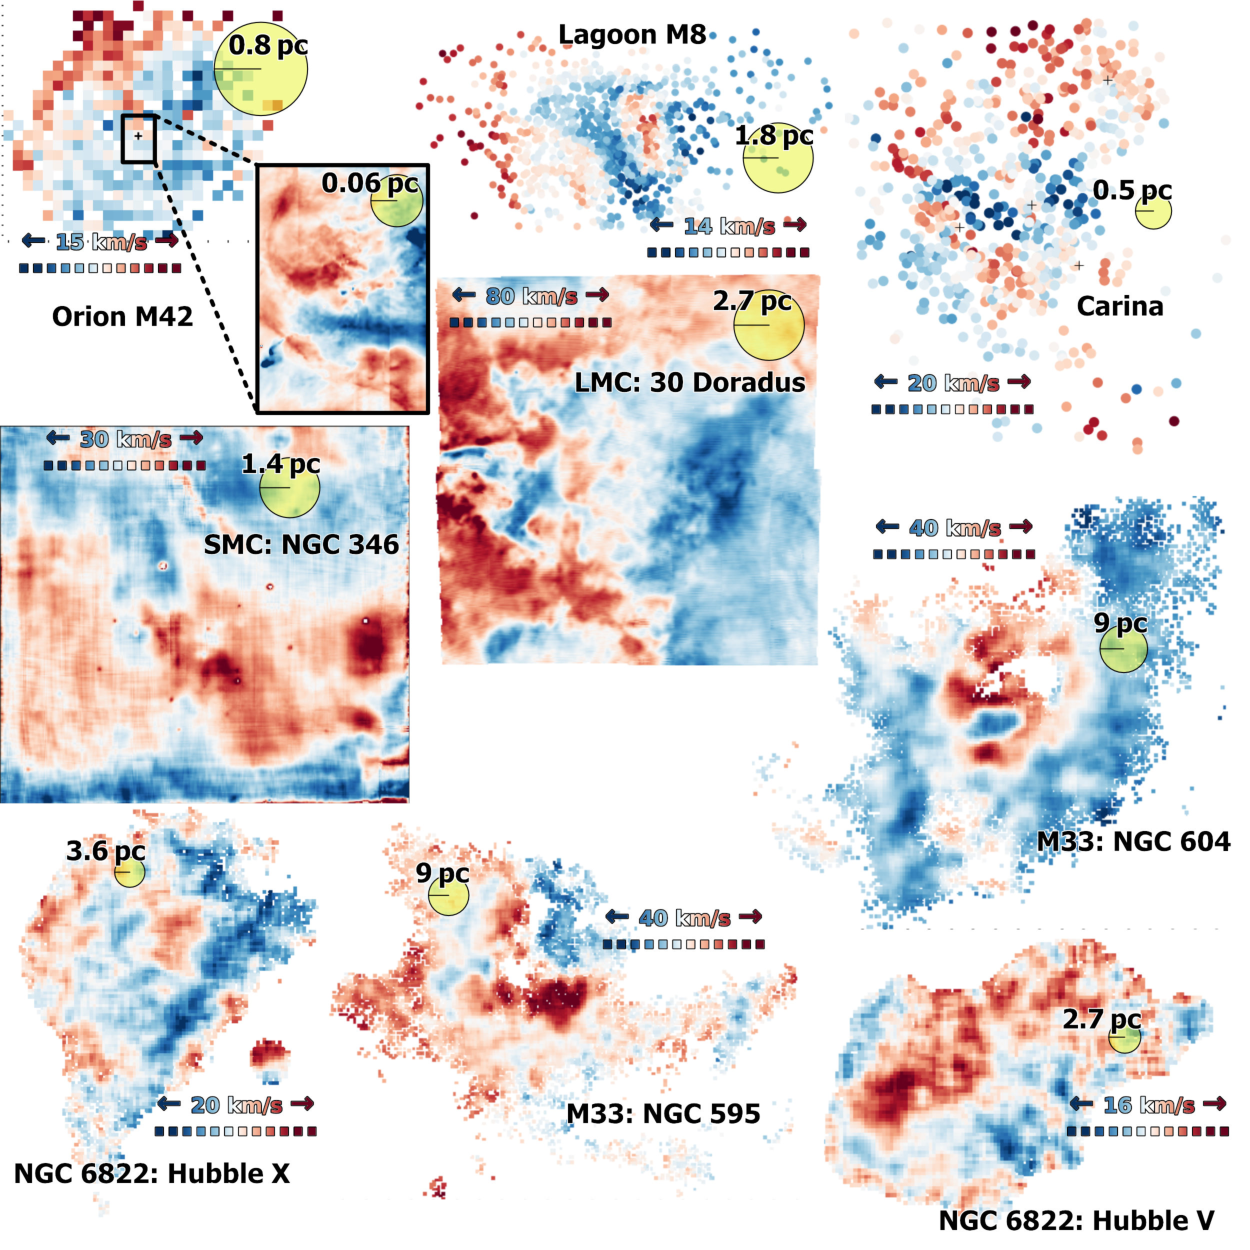
\includegraphics[width=\linewidth]{Figures/velocity-maps-mosaic}
  \caption{
    Maps of the mean \ha{} velocity for each of the regions in our sample.
    All velocities are relative to the systemic velocity of each region,
    with more negative velocities shown in blue and more positive velocities in red.
    The range of velocities is different for each region, as indicated on the individual maps.
    The correlation length of the velocity fluctuations in each region
    is shown as the radius of a yellow circle and labeled with its value in parsecs. 
  }
  \label{fig:velocity-maps}
\end{figure*}

Previous investigations of the centroid velocity structure function in \hii{} regions
have used a variety of methodologies, which makes it difficult to compare results
between different regions.  \citet{arthur2016turbulence} summarise historical results
for the Orion Nebula in their Table~5.
The most significant differences are seen when different emission line tracers are used,
but even when using the same line, there is some variance between different studies
in the derived values for both the velocity dispersion \(\sigma\pos\) and power-law slope \(m\).
It is therefore worthwhile to employ a uniform approach across a variety of different regions.
To that end, we have selected 9 \hii{} regions,
covering a broad range in size and luminosity,
for which good quality mapping of the \ha{} line exists in the literature
or in data archives.
Figure~\ref{fig:hii-regions} shows optical images of
each region in our sample
and Table~\ref{tab:regions-properties} lists their most important physical parameters.
The derived centroid \ha{} velocity maps are shown in Figure~\ref{fig:velocity-maps}.
Our sample includes three Milky Way regions
(at approximate distance of \num{0.5} to \SI{2}{kpc}),
two regions in the Magellanic Clouds (\num{50} to \SI{60}{kpc}),
and four regions in more distant galaxies of the Local Group
(\num{500} to \SI{800}{kpc}).
Further details of the observations are given in the following section.

\subsection{Spectroscopic datasets}
\label{sec:spectr-datas}

\newcommand\xx{\ensuremath{\boldsymbol{x}}}
Wherever possible, we calculate the centroid velocity \(V_c\)
directly as the normalized first velocity moment of the spectral line intensity profile
for each plane-of-sky position \(\xx\) on the nebula:
\(V_{c}(\xx) = M_1(\xx) / M_0(\xx)\).
The \(k\)th unnormalized moment \(M_k\) of the continuum-subtracted
spectral intensity profile \(I(v)\)
is defined as
\begin{equation}
  \label{eq:kth-moment}
  M_k = \int_{\Delta v} I(v) \, v^k \, dv
\end{equation}
where the Doppler velocity \(v\) is calculated according to
the \texttt{VOPT} convention
\citetext{Eq.~[32] of \citealt{Greisen:2006a}}:
\begin{equation}
  \label{eq:optical-velocity}
  v \equiv c\, (\lambda - \lambda_0) / \lambda_0 ,
\end{equation}
where \(\lambda\) is the observed wavelength,
\(\lambda_0\) is the rest wavelength, and \(c\) is the speed of light.
The spectral window \(\Delta v\) is chosen to be just large enough to include
the entire \ha{} emission line.
So long as the signal-to-noise is high enough,
this mean velocity can be calculated to a much higher precision
than the nominal velocity resolution of the spectrograph. 
In a few cases, as noted below, we are working with already reduced data,
which are provided in the form of Gaussian fits to the line profiles.
In the cases where multiple Gaussian components have been fitted,
we take the flux-weighted mean velocity of these components to be the centroid.

The observed RMS spectral line width \(\sigma'\) can likewise be found from
the second velocity moment as
\begin{equation}
  \label{eq:observed-sigma}
  \sigma'(\xx)^2  = [M_2(\xx) / M_0(\xx)] - V_{c}(\xx)^2 .
\end{equation}
However, many different broadening mechanisms contribute to this width,
including the finite spectral resolution \(\sigma_{\mathrm{ins}}\),
fine-structure splitting \(\sigma_{\mathrm{fs}}\),
and thermal Doppler broadening \(\sigma_{\mathrm{t}}\).
In the approximation that all these broadening mechanisms are independent
and described by Gaussian profiles, then the dispersion of
line-of-sight velocities due to bulk motions \(\sigma\los\) can be found
by subtracting these contributions in quadrature from the observed width:
\begin{equation}
  \label{eq:sigma-los}
  \sigma\los^2 = \sigma'^2 - \sigma_{\mathrm{ins}}^2 - \sigma_{\mathrm{fs}}^2 - \sigma_{\mathrm{t}}^2 .
\end{equation}
See sec~5.1 of \citet{Garcia-Diaz:2008a} for further details.

\subsubsection{Longslit echelle spectroscopy}
\label{sec:longsl-echelle-spect}

For the Orion Nebula, we use data obtained with the echelle spectrograph attached to the \SI{4}{m} telescope at Kitt Peak National Observatory (KPNO) initially published in
\citet{Doi:2004a}.
These observations cover a \(\SI{3}{arcmin} \times \SI{5}{arcmin}\) region of the
central (Huygens) part of the Orion Nebula.
The data consist of 96 North--South orientated \SI{300}{arcsec} slits,
uniformly spaced at \SI{2}{arcsec} intervals with a width of \SI{0.8}{arcsec}
with a velocity resolution of \SI{8}{km.s^{-1}}. 
For the centroid velocities, we use the intensity-weighted 
mean velocities calculated by \citet{Garcia-Diaz:2008a},
who used additional observations with East--West oriented slits
to refine the inter-slit velocity calibration. 
Unlike in the previous analysis of this dataset by \citet{arthur2016turbulence},
we do not mask out regions affected by known high-velocity outflows.
This decision was made for consistency with the analysis of more distant regions,
where such a masking out is not possible.

\subsubsection{Fabry-Pérot observations}
\label{sec:fabry-perot-etalaon}

We use the velocity field presented in \citet{1987A&A...176..347H} to analyze the Extended Orion Nebula \citetext{EON henceforth;  \citealp{2008Sci...319..309G}}.
the brightness following the southwest direction from the Huygens region.
The observational data was obtained using a Fabry-Pérot interferometer with a étalon separation of 0.5 mm on the 106 cm-Cassegrain telescope at Observatorium Hoher List. 
A number of fifteen interferograms have been taken with different pointing directions of the telescope's optical axis in the nebula with an exposure time between 10 and 40 minutes. 
The exposures are overlapped and fall into one square of a grid with a width of \SI{1}{arcmin} centered at \(\theta^{1}\)Ori C.   


\subsubsection{FLAMES multi-fiber spectroscopy}
\label{sec:flames-multi-fiber}

Archival data from \citet{Damiani:2016a} and \citet{Damiani:2017b} are used
to study the Carina Nebula and Lagoon Nebula, respectively.
These were obtained as a by-product of a study of young stars in their respective regions
as part of the Gaia-ESO Spectroscopic Survey \citep{Gilmore:2012v, Randich:2013m}
using VLT/FLAMES with the GIRAFFE and UVES spectrographs \citep{2002Msngr.110....1P}.
The spectra are from multiple discrete fiber positions in each nebula
(866 positions in Carina; 1089 in the Lagoon),
visible as colored disks in Figure~\ref{fig:velocity-maps}.
The angular separation between fibers varies across the maps with
average nearest-neighbor distance of \SI{21 \pm 17}{arcsec}.
The spectral resolution ranges from  \SI{6}{km.s^{-1}} (UVES) to \SI{16}{km.s^{-1}} (GIRAFFE).
We do not have access to the individual spectra, but instead use the
Gaussian fits to the line profiles from \citep{Damiani:2016a, Damiani:2017b},
obtained from data tables downloaded from the CDS Vizier service.\footnote{%
  \url{https://doi.org//10.26093/cds/vizier.35910074} and
  \url{https://doi.org//10.26093/cds/vizier.36040135}.}
For the Lagoon, we use single-Gaussian fits, while for Carina we take the
flux-weighted mean of the blue and red component of two-Gaussian fits.


\subsubsection{MUSE integral field spectroscopy}
\label{sec:muse-integral-field}

For the Magellanic Cloud regions 30~Doradus and NGC~346 we use data obtained
with the MUSE spectrograph \citep{Bacon:2010a, Bacon:2014a} on the VLT.\@
Each exposure consists of a \(300 \times 300\) pixel spectral image with a plate scale
of \SI{0.2}{arcsec.pixel^{-1}} and a spectral resolution of \SI{110}{km.s^{-1}}
at \ha{}.
For 30~Doradus, four separate exposures are mosaicked to give a square field of
size \(\SI{2}{arcmin}\) \citep{Castro:2018a}. 
We use centroid velocities of single Gaussian fits to the \ha{} line.\footnote{%
  Data kindly provided by Norberto Castro Rodríguez, priv.~comm.
}
For NGC~346, we use a single field that was observed in 2016 as part of
ESO observing program 098.D-0211(A) (P.I. W.-R.~Hamann).
We obtained the pipeline-reduced data cubes from the ESO data archive\footnote{%
  \url{http://archive.eso.org/wdb/wdb/eso/eso_archive_main/query?prog_id=098.D-0211(A)}
}
and extracted the \ha{} profile using tools in the MPDAF python library.\footnote{
  \url{https://mpdaf.readthedocs.io/en/latest/}
} 

\subsubsection{TAURUS-II Fabry-Perot interferometer}
\label{sec:taurus-ii-fabry}

The archival data for the extragalactic giant regions (GEHRs), NGC 604, NGC 595, Hubble X and Hubble V was obtained with the Fabry Perot TAURUS-II instrument
\citep{Gordon:2000v}
on the \SI{4.2}{m} William Herschel Telescope (WHT) and was retrieved from the La Palma archive\footnote{\url{http://casu.ast.cam.ac.uk/casuadc/ingarch}}.
The IPCS-II detector was used with a etalon of \SI{125}{\mu m}.
Each data cube is \(256 \times 256 \times 100\) with a spatial scale of \SI{0.26}{arcsec.pixel^{-1}} with a total integration time of \SI{3600}{s} (\SI{36}{s} per frame).
For more details on the observational setup see table~1 of \citet{sabalisck1995supersonic}.
The reduction and analysis was done with the packages TAUCAL y TAUFITS \citep{1992ASPC...25..445L} and the emission spectrum was adjusted with a Gaussian fit.
The NGC~604 observations were previously reported and analyzed in
\citet{sabalisck1995supersonic}, \citet{Medina-Tanco:1997a} and \citet{Melnick:2021x}.


\subsection{Physical properties of the sample regions}
\label{sec:regions-milky-way}

\begin{table}
\begin{center}\caption{Summary of properties of our \hii{} region sample. Diameters taken from Table 2 of \citet{1984ApJ...287..116K}. Mean non-thermal linewidth values, \(\langle \sigma\los \rangle\), shown here are corrected considering equation \eqref{eq:sigma-los} which takes into account \(\sigma_{\mathrm{fs}}\). Non-corrected \(\langle \sigma\los \rangle\) values and other properties references are mentioned in the text. }
\begin{tabular}{cCCCC}\toprule
\hii{}    &  \text{Distance,}\ d & \text{Diameter,}\ D & \log L(\ha) &  \langle \sigma\los \rangle \\
  Region    &  [\si{kpc}]          &  [\si{pc}]    &  [\si{erg.s^{-1}}]            &    [\si{km.s^{-1}}]  \\ 
\midrule
Orion     & 0.44 \pm 0.02  & 5 \pm 0.5    &    37.18       &    9.9 \pm 1.2\FNa        \\
Lagoon    & 1.25 \pm 0.12   & 25 \pm 2.5      &    37.47    &   11.2 \pm 1.6    \\
Carina    & 2.35 \pm 0.05   & 200 \pm 20      &    38.54    &   18.6 \pm 3.3\FNa      \\
30 Dor    & 50.0 \pm 0.2    & 370 \pm 37    &    39.46    &     21.7 \pm 2.2    \\
NGC 346   & 62 \pm 1        & 220 \pm 22      &    38.77    &    9.6 \pm 1.0     \\
Hubble X  & 490 \pm 40      & 160 \pm 16      &    38.21    &   10.0 \pm 0.02\\
Hubble V  & 490 \pm 40      & 130 \pm 13      &    38.3     &    9.8 \pm 0.03     \\
NGC 595   & 820 \pm 30      & 400 \pm 40      &    38.95    &   16.5 \pm 0.1     \\
NGC 604   & 820 \pm 30      & 400 \pm 40      &    39.42    &   17.5 \pm 0.30     \\
\bottomrule
\multicolumn{5}{l}{\FNa{}Value obtained from our observations.}
\end{tabular}\label{tab:regions-properties}
\end{center}
\end{table} 

Table~\ref{tab:regions-properties} summarizes the properties of the regions in our sample
with data taken from the literature. Further details on each individual source and their references are given in Appendix~\ref{sec:notes-individual-hii}.

%%%%%%%%%%%%%%%%%%%%%%%%%%%%%%%%%%%%%%%%%%%%%%%%%%%%%%%%%%%%%%%%%%%%%%%%%%%%%%%%%%%%%%%%%%%%%%%%%%%%
%%%%%%%%%%%%%%%%%%%%%%%%%%%%%%%%%%%%%%%%%%%%%%%%%%%%%%%%%%%%%%%%%%%%%%%%%%%%%%%%%%%%%%%%%%%%%%%%%%%%%%%

\section{Plane-of-sky velocity fluctuations}\label{sec:met}

Figure~\ref{fig:velocity-maps} shows maps of the \ha{} centroid velocity
\(V_c\) for each \hii{} region in our sample,
calculated as described above in section~\ref{sec:spectr-datas}
and after subtracting the mean systemic velocity,
\(\left\langle V_c\right\rangle\) in each case.
% The color scheme ranges from the most negative velocities in blue
% to the most positive velocities in red,
% but the amplitude of the velocity fluctuations differs considerably between regions,
% as indicated by the color scale bar on each map,
% ranging from \SI{\pm 7}{km.s^{-1}} for the Lagoon
% up to  \SI{\pm 40}{km.s^{-1}} for 30~Doradus.
The overall amplitude of the plane-of-sky
velocity fluctuations can be characterized by a dispersion,
\(\sigma\pos\), defined as:
\begin{equation}
  \label{eq:sig-pos}
  \sigma^2\pos =
  \left\langle 
  \bigl[ V_c (\xx_i) -\langle V_ c\rangle  \bigr]^2
  \right \rangle ,
\end{equation}
where the average is performed over all observed points \(i\)
in a given map.
Note that \(\sigma\pos\) is also the RMS width of
the probability density function (PDF) of \(V_c\).
This PDF for each region is shown in Figure~\ref{fig:pdfs}
on a common velocity scale and arranged in order of decreasing \(\sigma\pos\).
It can be seen that the amplitude of the
velocity fluctuations varies considerably between regions,
with \(\sigma\pos\) in 30~Dor being more than 5 times higher than in 
nearby regions such as Orion.

All of the PDFs are significantly non-Gaussian
and many show evidence of a multi-modal structure.
Some, such as Orion core and Hubble~V, show a single dominant velocity component,
but most show several distinct peaks,
as many as four in the case of Carina.
There is no clear tendency for the number of identifiable velocity components
to increase with increasing velocity dispersion.
Instead, both the widths of the individual peaks and the separation between them
seem to increase in tandem.
For most regions the PDFs are approximately symmetrical,
but two regions show significant skewness:
Orion~core has a smooth asymmetrical tail towards the blue,
whereas NGC~346 has one towards the red.

\begin{figure*}
 \centering
 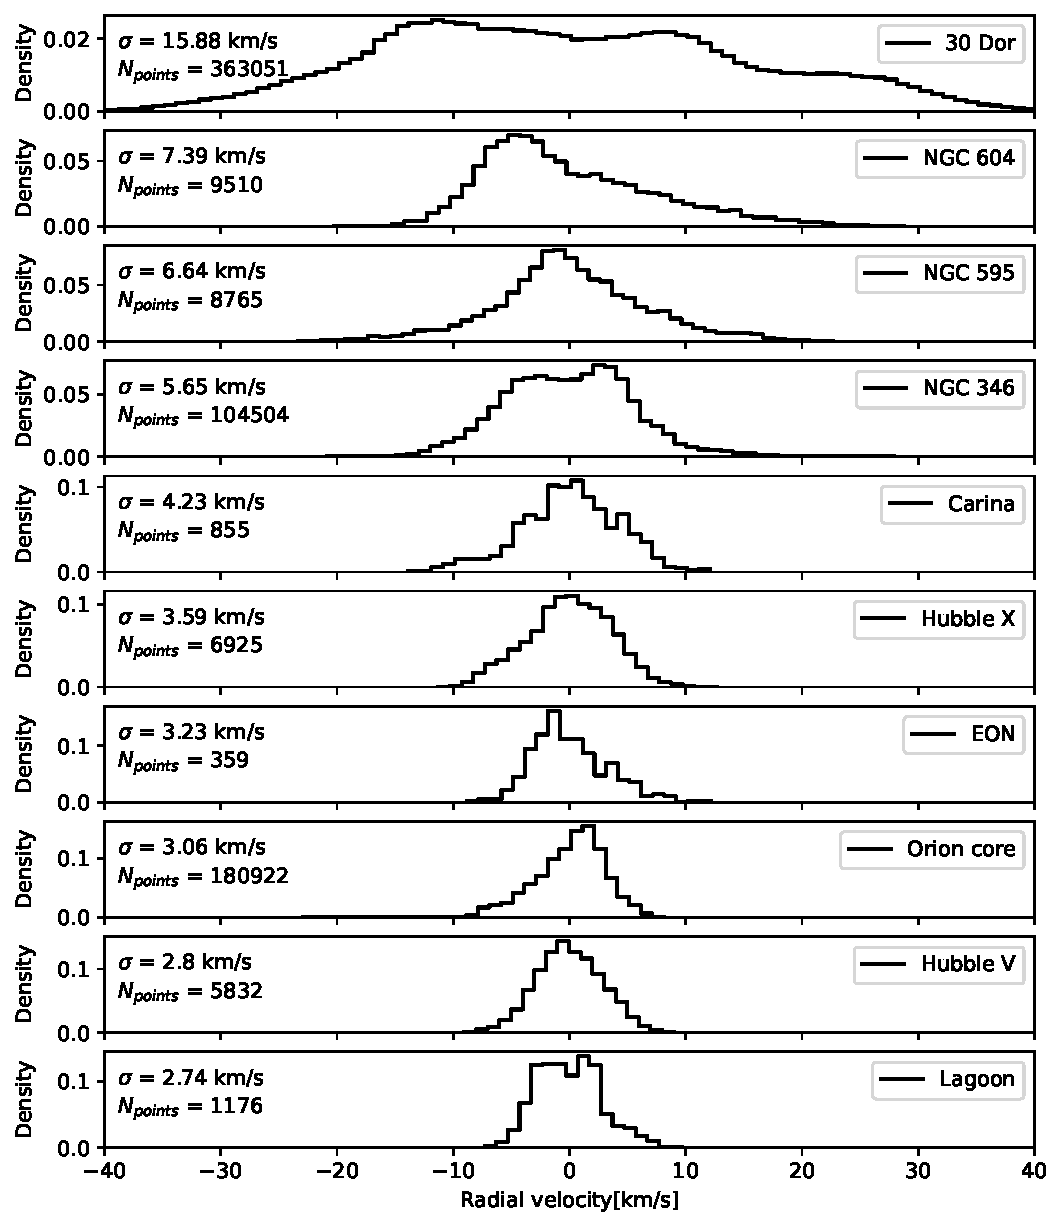
\includegraphics[width=5in]{Figures/pdfs}\par
 \caption{
   Histograms of the plane-of-sky variation in the \ha{} centroid velocities.
   Each panel shows the fraction of the observed spatial points
   (pixels or fiber positions)
   with a given velocity offset from the mean systemic velocity of each region.
   The RMS width \(\sigma\pos\) of each distribution is marked,
   as is the number of spatial points.
   The bin width is \SI{1}{km.s^{-1}} and the regions are arranged
   in order of decreasing \(\sigma\pos\).
 }
 \label{fig:pdfs}
\end{figure*}


\subsection{The second-order structure function}
\label{sec:second-order-struct}


In order to probe the dependence of the velocity fluctuations
on spatial scale,
the primary tool that we employ is
the second order structure function of differences in velocity centroids,
$B(r)$, which is a function of the scalar separation or lag, \(r\),
between two points on the plane of the sky:
%
\newcommand\Abs[1]{\vert #1\vert}
\begin{equation}\label{eq:Br}
  B(r) = \left\langle 
  \bigl[
  V_{c}(\xx_j) - V_{c}(\xx_i)
  \bigr]^{2} \right \rangle_{\Abs{\xx_j - \xx_i\!} \ \approx \ r} \ .
\end{equation}
The averaging is performed over all pairs of points
\((i, j)\)
whose scalar separation \(\Abs{\xx_j - \xx_i}\) is close to \(r\),
irrespective of the orientation of the separation vector.
In practice, we achieve this by binning the separations with a constant
logarithmic width of \SI{0.05}{dex}.

We will also employ the related quantity of the
normalized spatial autocovariance or autocorrelation function:
\begin{equation}
  \label{eq:autocovar}
  C(r) = \frac{1}{\sigma^2\pos}\left\langle 
  \bigl[
  V_{c}(\xx_j) \  V_{c}(\xx_i)
  \bigr] \right \rangle_{\Abs{\xx_j - \xx_i\!} \ \approx \ r} \ .
\end{equation}
If the fluctuations are perfectly spatially homogeneous, then the
two quantities are related \citep{1984ApJ...277..556S} as:
\begin{equation}\label{eq:functional}
  B(r) = 2\sigma^2\pos \bigl[   1 - C(r)\bigr] .
\end{equation}
In less ideal situations, then \(B(r)\) is to be preferred since it is
relatively unaffected by non-stationary effects
such as large-scale linear gradients 
\citep{1984ApJ...277..556S}.
Nonetheless, \(C(r)\) is more amenable to heuristic reasoning in some cases,
which we will take advantage of below.


\subsection{A heuristic model for the structure function}
\label{sec:methods-apply}

\begin{figure*}
 \centering
 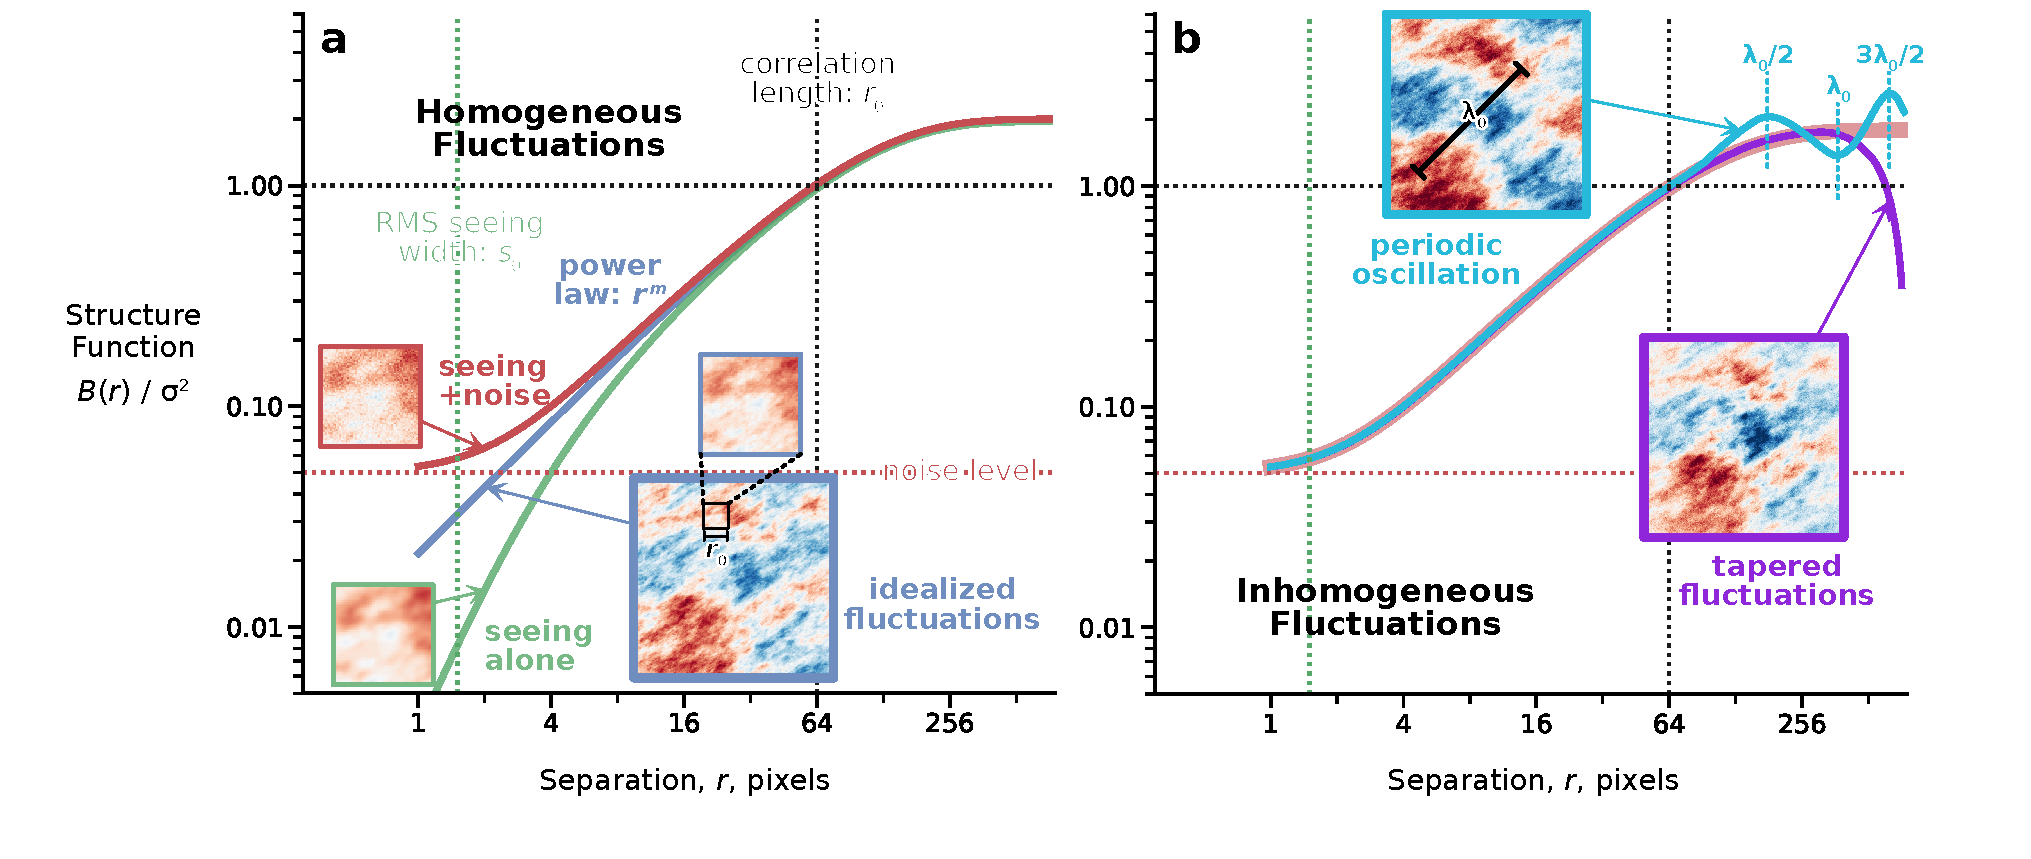
\includegraphics[width=\linewidth]{Figures/model-strucfunc-annotated}\par
 \caption{
   Example of the model structure function for homogeneous fluctuations,
   together with a realization of the corresponding velocity field
   on a \(512 \times 512\) pixel grid.  
   (a)~Idealized structure function (blue line)
   for the parameters \(m = 1\) and \(r_0 = \SI{64}{pixels}\).
   Red and green lines show the effects of observational limitations
   at small scales (seeing and noise)
   and at large scales (finite-map effects).
   (b)~Examples of inhomogeneous effects at large scales,
   which are not included in the model structure function.
 }
 \label{fig:model-strucfunc}
\end{figure*}

A common property of homogeneous fluctuating velocity fields is that neighboring points tend to have similar velocities
(\(C(r) \approx 1\) for small \(r\)),
whereas points that are far apart may have very different velocities
(\(C(r) \ll 1\) for large \(r\)).
The value of the separation that corresponds to
the transition between these two regimes
is called the correlation length, \(r_0\).
In the simplest case,
two points separated by \(r \gg r_0\) have totally uncorrelated velocities
in the sense that knowledge of the velocity at the first point is of
no help in predicting the velocity at the second point.
At scales smaller than \(r_0\), the fluctuations often show a power-law behavior
as a function of \(r\).

In order to capture these two behaviors,
we therefore propose the following idealized 2-parameter model
for the autocorrelation function:
%
\begin{equation}\label{eq:new-correlation-form}
  C\model(r;\ r_0, m) = 2^{- \left( r/r_0 \right)^m} 
\end{equation}
%
in which \(r_{0}\)\ is the correlation length (see above)
and \(m\) is the power-law slope at small scales.
This is constructed so that \(C\model(r) = 1/2\) at \(r = r_0\),
while the exponential form ensures that \(C(r)\) rapidly approaches zero
for larger separations.
We assume the validity of equation~\eqref{eq:functional} to determine the structure function
from this model autocorrelation function:
\begin{equation}
  \label{eq:model-strucfunc-ideal}
  B\model(r) = 2\sigma^2\pos \left[
    1 - 2^{- \left( r/r_0 \right)^m} 
  \right]
\end{equation}
This has the following properties:
\begin{enumerate}[1.]
 \item Small scales: \(B\model(r) \propto r^m\) for \(r \ll r_0\);
 \item Correlation scale: \(B\model(r_0) = \sigma\pos^2\);
 \item Large scales: \(B\model(r) \to 2 \sigma\pos^2\) for \(r \gg r_0\).
 \end{enumerate}
An example is shown by the blue line in Figure~\ref{fig:model-strucfunc}a.
 
In a previous paper, we used a different functional form
\citetext{See Fig.~13 of \citealp{arthur2016turbulence}}:
\(C(r) = 1/[1+(r/r_{0})^{m}]\), as proposed in \citet{1984ApJ...277..556S},
which behaves identically to equation~\eqref{eq:new-correlation-form}
in the first two regimes, but is more gradual in its approach
to the large-scale asymptote of \(2 \sigma\pos^2\).
However, we find that equation~\eqref{eq:new-correlation-form}
provides a much improved fit to the observed structure functions
of our sample regions (see following section). 


% The term \(r_{0}\)\ is the correlation length where the value of separation \(r\) reach the value of \(\sigma^2\) in the structure function and $m$ is the power-law index that fits the inertial scale.
% In an idealized case at scales larger than \(r_{0}\)\ the structure function flattens as it tends towards the asymptotic value of 2\(\sigma^2\) \citep{arthur2016turbulence}.
% This substitutes the previously \(C(r) = 1/[1+(r/r_{0})^{m}]\) from \citet{1966igd..book.....K} and
% \citet{1984ApJ...277..556S}.

\subsubsection{Effects of observational limitations at small spatial scales}
\label{sec:effect-observ-limit}

Two observational effects can modify the observed structure function at the smallest scales.
The first is the blurring of the observed image by atmospheric seeing,
which tends to reduce \(B(r)\) for small \(r\).
In Appendix~\ref{sec:effects-seeing-struc}, we perform numerical experiments
with synthetic velocity fields and find that
a good approximation to the effects of seeing is to multiply
the model structure function by a factor:
\begin{equation}\label{eq:ffs}
   S(r) = \frac{
    e^{-s_0 / r_0}
  }{
    1+(2s_0 / r)^{2 / 3}
  } ,
\end{equation}
where \(s_0\) is the RMS width of the seeing profile\footnote{%
  Note that the full-width half maximum (FWHM) seeing width is
  \(2 (2 \ln 2)^{1/2} s_0 \approx 2.35 s_0\).
}
and \(r_0\) is the correlation length.
An example is shown by the green line in Figure~\ref{fig:model-strucfunc}a.
The effect of seeing is to make the structure function 
bend down away from the idealized power law, 
becoming increasingly steep at scales smaller than \(s_0\),
but having a noticeable effect at scales up to \(10 \times s_0\).

The second effect is the presence of instrumental noise
in the observational measurements,
such as Poisson noise from photon-counting statistics. 
Although this affects all scales,
it is most noticeable for small separations,
where the intrinsic structure function is smallest.
If the noise is spatially uncorrelated
(equal and independent uncertainties in the velocity
measurement of each pixel),
then its contribution to the structure function is independent of separation,
which means it can be represented as a constant term \(B\noise\).

Combining both the effects of seeing and noise yields the corrected
model structure function:
\begin{equation}
  \tilde{B}\model(r) = B\model(r) \,  S(r) + B\noise
  \label{eq:sf-functional}
\end{equation}
An example of this equation is shown by the red line in Figure~\ref{fig:model-strucfunc}.
Note that seeing and noise have opposite effects on the slope
of the structure function at intermediate scales:
seeing tends to steepen the slope, while noise tends to flatten it.
This can lead to a degeneracy between these two parameters
when fitting observations over a limited range of separations.

\subsubsection{Effects of observational limitations at large spatial scales}
\label{sec:effects-observ-limit-large}

In Appendix~\ref{sec:finite-box-effects} we consider the effects
on the structure function of the finite size \(L\) of the observational map.
If the true correlation length \(r_0\) is more than a small fraction of the map size
(approximately, \(r_0 > 0.1 L\)),
then the apparent velocity variance measured directly from the data
is less than the true \({\sigma\pos}^2\) of the underlying fluctuations
(see Figure~\ref{fig:finite-box-effect}).
This is because the observed map is not large enough to sample
the full range of velocity variations.
At the same time, the apparent correlation length is smaller
than the true value.
However, this does not mean that the model structure function needs to be modified.
In the appendix we show that the model fitting is capable of determining the true fluctuation variance
and true correlation length (both to within 10\%),
so long as \(L > 3\, r_0\).
This is a significant improvement over direct empirical measurement,
which requires \(L > 10\, r_0\) in order to be accurate
(compare panels a and b of Figure~\ref{fig:finite-box-effect}).

\subsubsection{Additional effects omitted from the model structure function}
\label{sec:limit-model-struct}

For separations that are comparable to the diameter \(D\) of the \hii{} region,
then the supposition of homogeneity may break down.
For instance, if the amplitude of the velocity fluctuations is higher
in the core of the region than in the outskirts,
then the autocorrelation function will be U-shaped
since all separations with \(r > D/2\) must be between two points in the outskirts,
which will tend to be relatively well correlated simply because both velocities
will be close to the mean.
This yields a corresponding downturn in the structure function at the largest scales.

Another example is if there were a periodic velocity fluctuation,
with spatial wavelength \(\lambda\),
then the autocorrelation function would become negative for \(r \approx \lambda/2, 3 \lambda / 2, \dots\),
which yields periodic peaks in the structure function.
Both effects are illustrated in Figure~\ref{fig:model-strucfunc}b.
Neither of them can be captured by our model structure function,
which assumes that the autocorrelation is strictly positive
and monotonically decreasing with \(r\).
We deal with this limitation by not attempting to model scales larger than \(L / 2\),
where the influence of these effects will be greatest.

\section{Structure function fits}
\label{sec:results}

\newlength\SFwidth
\setlength\SFwidth{0.45\textwidth}
\newcommand\SFtwograph[2]{%
  \includegraphics[width=\SFwidth]{Figures/sf-emcee-#1}
  &  \includegraphics[width=\SFwidth]{Figures/sf-emcee-#2}
}
\newcommand\SFtwocorner[2]{%
  \includegraphics[width=\SFwidth]{Figures/corner-emcee-#1}
  &  \includegraphics[width=\SFwidth]{Figures/corner-emcee-#2}
}


\newcommand\sffigg[2]{%
  \begin{tabular}{@{}ll@{}}
    (a)& (b)\\
    \SFtwograph{#1}{#2}
  \end{tabular}%
}
\newcommand\sffigggg[4]{%
  \begin{tabular}{@{}ll@{}}
    (a)& (b)\\
    \SFtwograph{#1}{#2}\\
    (c)& (d)\\
    \SFtwograph{#3}{#4}\\
  \end{tabular}%
}
\newcommand\sfcfig[1]{%
  \includegraphics[width=\SFwidth]{Figures/corner-emcee-#1}%
}  
\newcommand\sfcfigg[2]{%
  \begin{tabular}{@{}ll@{}}
    (a)& (b)\\
    \SFtwocorner{#1}{#2}
  \end{tabular}%
}
\newcommand\sfcfigggg[4]{%
  \begin{tabular}{@{}ll@{}}
    (a)& (b)\\
    \SFtwocorner{#1}{#2}\\
    (c)& (d)\\
    \SFtwocorner{#3}{#4}\\
  \end{tabular}%
}

\begin{figure*}
  \centering
  \sffigggg{OrionS}{OrionLH}{M8}{CarC}
  \caption{
    Second-order structure functions
    for velocity centroid images
    of the \ha{} emission line
    from Galactic \hii{} regions.
    The observed structure function \(B\obs(r)\) is shown by 
    blue symbols, with filled symbols indicating those points
    that are used to constrain the model fits.
    The full model is shown in orange,
    while the underlying ideal model
    (without the effects of seeing or noise)
    is shown in green.
    See text for details of the fitting process.
    (a)~Inner Orion Nebula.
    (b)~Extended Orion Nebula.
    (c)~M8, the Lagoon Nebula.
    (d)~Carina Nebula.
  }
  \label{fig:strucfunc-fit-Galactic}
\end{figure*}

\begin{table}
  \centering
  \caption{Bounds of allowed values for parameters in model fits}
  \label{tab:parameter-ranges}
  \newlength\partabwidth
  \setlength\partabwidth{0.8\linewidth}
  \begin{tabular*}{\partabwidth}{
    l @{\extracolsep{\fill}}
    r 
    r
    }
    \toprule
    Parameter & Lower & Upper\\
    \midrule
    \(\sigma^2\) & \(0.25\, \max [B\obs]\)& \(2\, \max [B\obs]\)\\
    \(r_0\) & \(0.01\, L\) & \(2\, L\)\\
    \(m\) & \(0.5\) & \(2.0\) \\
    \(s_0\) & \SI{0.1}{arcsec}& \SI{1.5}{arcsec}\\
    \(B\noise\) & \(0\) & \(3\, \min [B\obs]\) \\
    \bottomrule
    \multicolumn{3}{@{}p{\partabwidth}@{}}{
    Note: \(\max[B\obs]\) and \(\min[B\obs]\) are over all bins in the observed structure function with \(r < L/2\).
    }
  \end{tabular*}
\end{table}

\begin{figure}
  \centering
  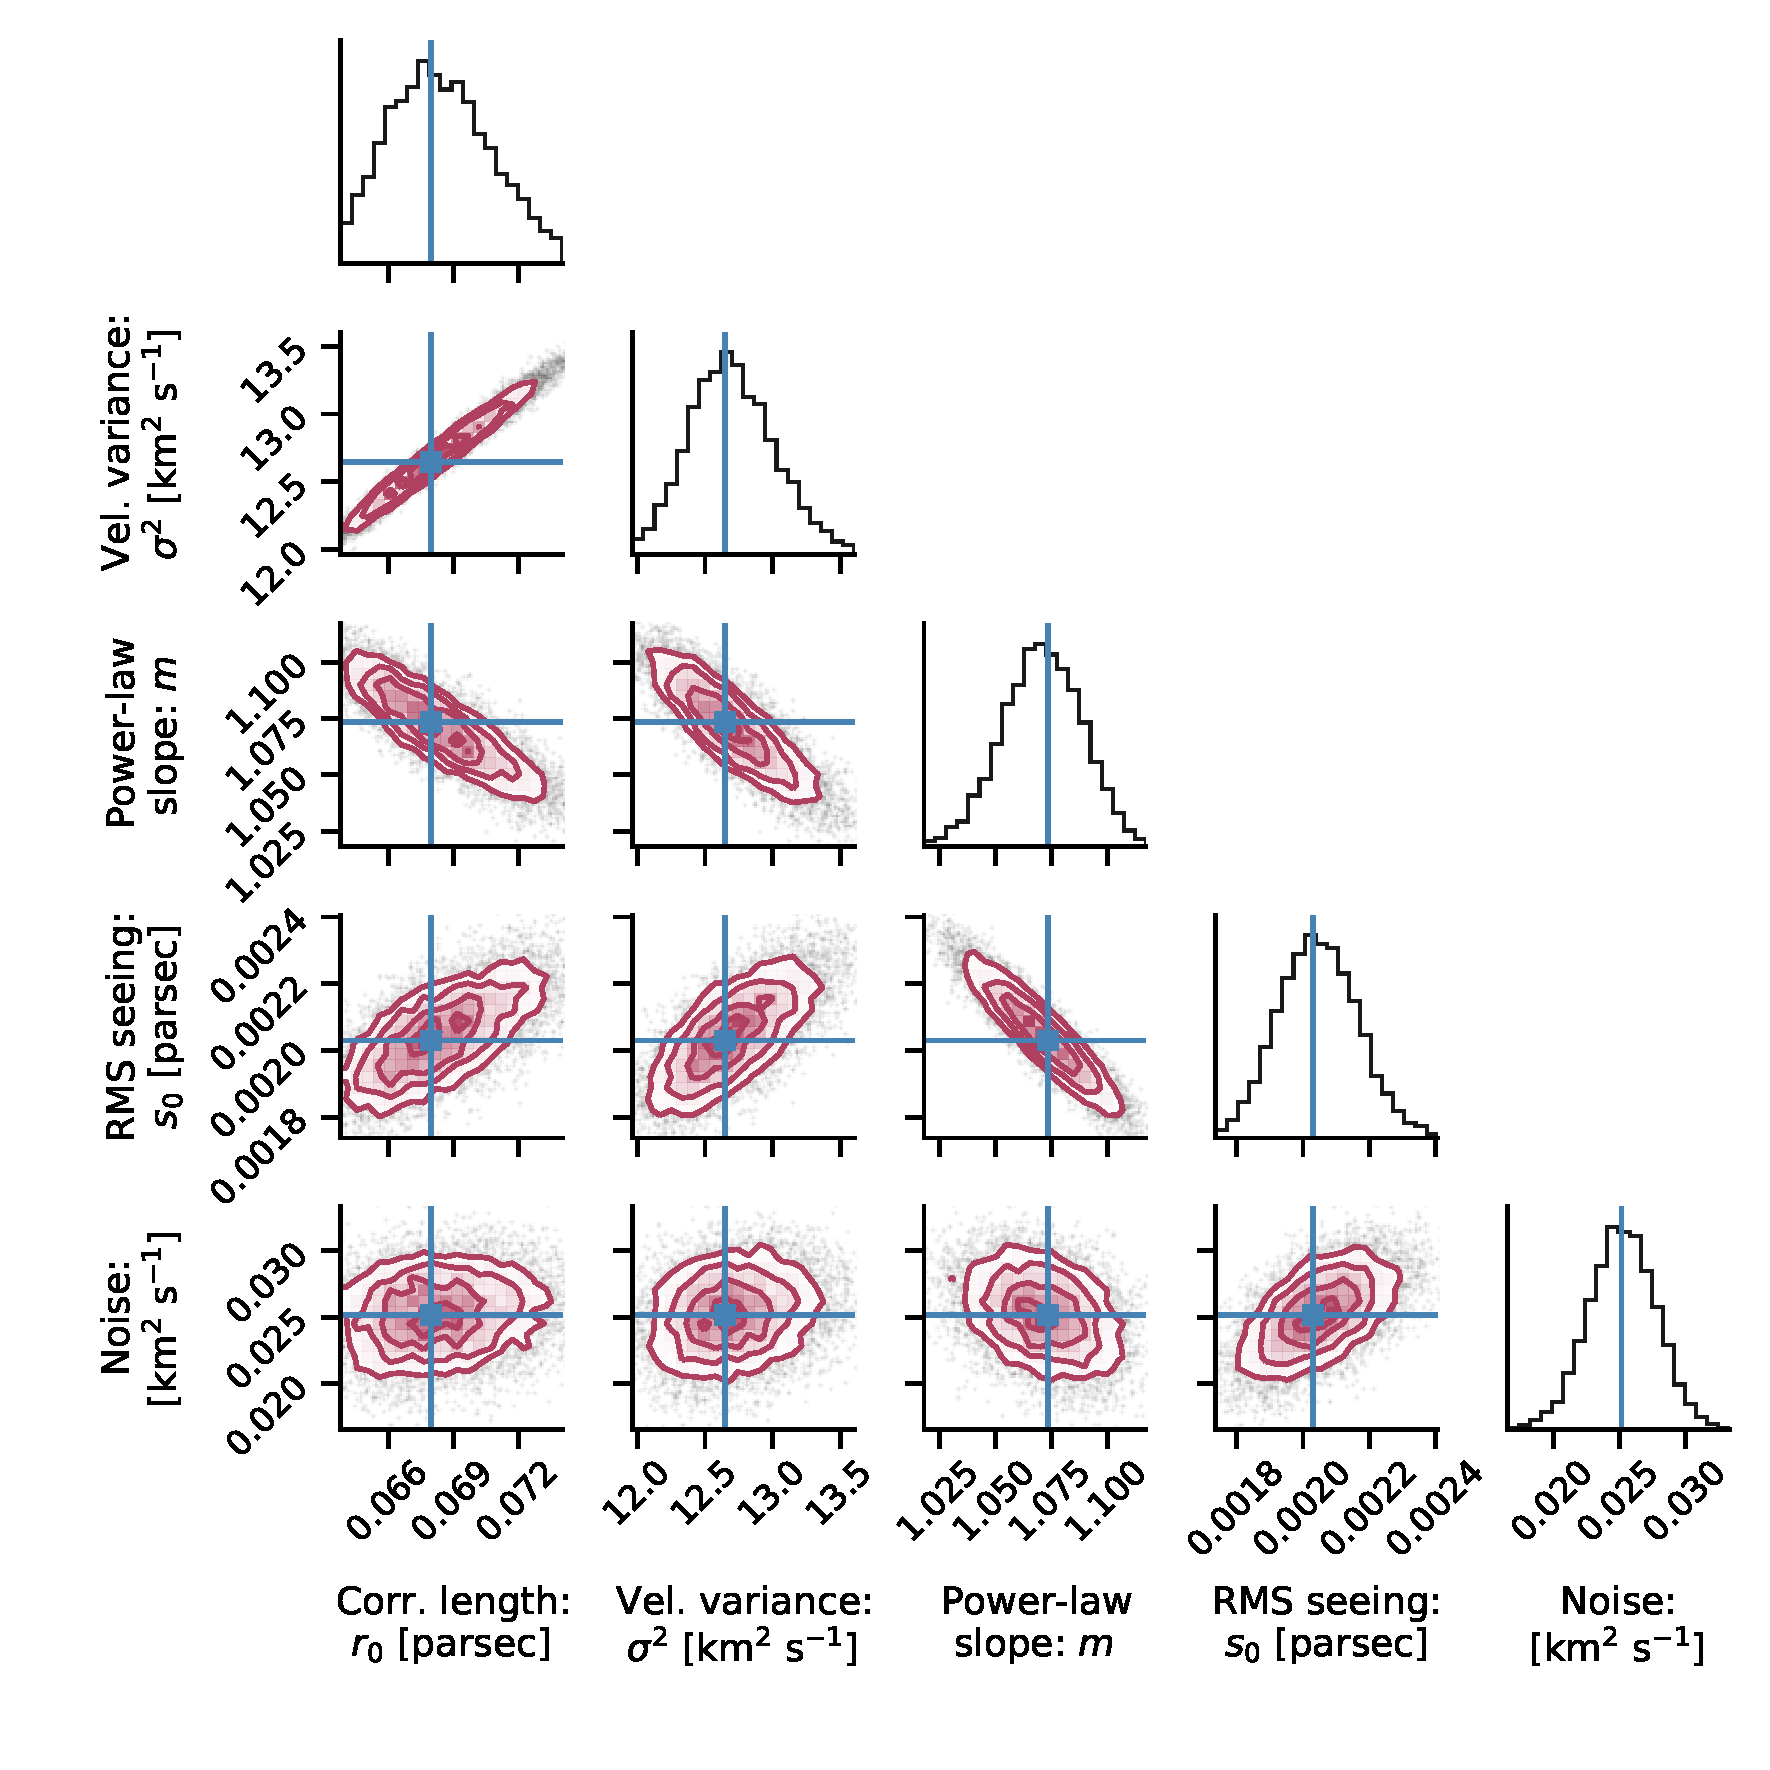
\includegraphics[width=\SFwidth]{Figures/corner-emcee-OrionS}
  \caption{
    Example corner plot of covariances between
    model parameters of fits to the \ha{} structure function.
    The example shown is for Orion,
    while figures for the remaining regions are given in
    Appendix~\ref{sec:addit-covar-corn}.
    Plots on the diagonal show the 1-dimensional histogram
    of the posterior distribution of each parameter
    (labeled at bottom),
    as calculated by the MCMC method,
    assuming a uniform prior distribution
    within the limits given in Table~\ref{tab:parameter-ranges}.
    Off-diagonal plots show the 2-dimensional histogram of the
    joint posterior distribution each pair of parameters.
  }
  \label{fig:corner-example-Orion}
\end{figure}


\begin{figure*}
  \centering
  \sffigg{Dor}{N346}
  \caption{
    Same as figure~\ref{fig:strucfunc-fit-Galactic}
    except for Magellanic Cloud \hii{} regions.
    (a)~30 Doradus in the LMC.
    (b)~NGC~346 in the SMC.    
  }
  \label{fig:strucfunc-fit-MC}
\end{figure*}

\begin{figure*}
  \centering
  \sffigggg{HV}{HX}{N595}{N604H}
  \caption{
    Same as figure~\ref{fig:strucfunc-fit-Galactic}
    except for \hii{} regions in more distant
    Local Group Galaxies.
    (a)~Hubble~V in NGC~6822.
    (b)~Hubble~X in NGC~6822.
    (c)~NGC~595 in M33.
    (d)~NGC~604 in M33.
  }
  \label{fig:strucfunc-fit-ExtraGal}
\end{figure*}


\newcommand\PM[2]{\ensuremath{\substack{+#1\\-#2}}}
%\newcommand\FNa{\textsuperscript{a}}
\begingroup
\setlength{\tabcolsep}{6pt} % Default value: 6pt
\renewcommand{\arraystretch}{1.5} % Default value: 1
%% In Emacs we can use M-x align-current to align the table on the & symbols after editing
\begin{table*}
\begin{center}
  \caption{
    Best-fit model parameters and 95\% credibility intervals
    for fits to observed structure functions
  }
  \begin{tabular}{l RRRRRR  @{\hspace{6\tabcolsep}} RRR}
    \toprule
Region   & \sigma^2\pos            & B_{\text{noise}}       & s_0 (\text{RMS})          & r_0                    & L         & m                   & L/r_0 & s_0 / r_0 & s_0 (\text{FWHM}) \\
         & [\si{km^2.s^{-2}}] & [\si{km^2.s^{-2}}]     & [\si{pc}]                 & [\si{pc}]              & [\si{pc}] & [-]                 & [-]   & [-]       & [\text{arcsec}]   \\
\midrule
30 Dor   & 297\PM{40}{20}     & 6.2\PM{1.6}{1.6}       & 0.12 \PM{0.06}{0.03}       & 4.0\PM{1.0}{0.5}       & 31        & 0.85\PM{0.08}{0.13} & 8     & 0.03      & 1.2\PM{0.7}{0.4}  \\
NGC 604  & 84\PM{22}{10}      & <1.0                  & 1.6 \PM{1.0}{0.6}         & 12\PM{6}{5}            & 173       & 0.77\PM{0.20}{0.22} & 14    & 0.13      & 1.0\PM{0.5}{0.4}  \\
NGC 595  & 53\PM{5}{2}        & <3.3                   & <1.0         & 11\PM{1}{1}            & 196       & 1.36\PM{0.10}{0.15} & 18    & <0.04      & <0.5 \\
NGC 346  & 33\PM{3}{2}        & 0.8\PM{0.07}{0.07}       & 0.08 \PM{0.02}{0.02}      & 2.4\PM{0.3}{0.2}       & 20        & 0.95\PM{0.05}{0.07} & 8    & 0.04      & 0.7\PM{0.2}{0.1}  \\
Carina   & 18\PM{2}{2}        & <4.7                   & <0.010                    & 0.6\PM{0.1}{0.1}       & 20        & 1.16\PM{0.28}{0.18} & 33    & <0.01     & <3.4              \\
Hubble X & 15\PM{3}{1}        & <0.8                   & <0.55        & 4.0\PM{0.5}{0.2}       & 78        & 1.02\PM{0.06}{0.23} & 20    & <0.07      & <0.5 \\
Orion    & 13\PM{1}{1}        & 0.030\PM{0.005}{0.005} & 0.0020\PM{0.0002}{0.0002} & 0.068\PM{0.006}{0.004} & 0.5       & 1.07\PM{0.03}{0.04} & 7     & 0.02      & 1.8\PM{0.2}{0.2}  \\
Hubble V & 10\PM{3}{1}        & <0.65                  & <0.67        & 3.6\PM{0.5}{1.0}       & 61        & 0.81\PM{0.07}{0.28} & 17    & <0.14      & <0.65  \\
Lagoon   & 7\PM{1}{1}         & 0.45\PM{0.2}{0.3}      & <0.010                     & 1.0 \PM{0.2}{0.1}      & 16        & 1.26\PM{0.20}{0.20} & 16    & <0.01     & <3.5              \\
EON      & 5\PM{0.6}{0.4}         & 4.4\PM{0.9}{0.7}      & 0\FNa                     & 0.5\PM{0.2}{0.1}       & 3         & 1.0\FNa             & 6     & 0\FNa     & 0\FNa             \\
  \bottomrule
  \multicolumn{9}{l}{\FNa{}Assumed value.}
\end{tabular}\label{tab:Res}
\end{center}
\end{table*}
\endgroup
%%% Local Variables:
%%% mode: latex
%%% TeX-master: "strucfunc_paper"
%%% End:



In order to provide a uniform description of the velocity fluctuations,
we fit the model structure function
\(\tilde{B}\model(r)\) of equation~\eqref{eq:sf-functional}
to each \hii{} region in our sample.
Results are shown in Figures~\ref{fig:strucfunc-fit-Galactic}, \ref{fig:strucfunc-fit-MC},
and~\ref{fig:strucfunc-fit-ExtraGal}, arranged in order of increasing distance.
Best-fit values for the model parameters,
together with 95\% credibility range,
are given in Table~\ref{tab:Res}.
After describing the methods used to
measure the structure function and fit the model (section~\ref{sec:techn-deta-model}),
we give details of the results in the example case of
the inner Orion Nebula (\ref{sec:example-results-orion})
and a broad overview of the results for other regions (\ref{sec:results-model-fitt}).
Further details of the results for individual regions are
given in Appendix~\ref{sec:notes-individual-hii}.

\subsection{Technical details of structure function measurement and fitting}
\label{sec:techn-deta-model}

For the observational values (\(B\obs(r)\); blue symbols),
the structure function is the average value of equation~\eqref{eq:Br}
over all pairs of points that contribute to each radial bin.
The uncertainty of each bin (blue error bars) is estimated
as the standard deviation of these values divided by the square root of
the number of contributing pairs.
\textit{But this is not true -- we use constant fractional error with adjustments for small and large separations.}
For most sources a fixed bin size of \SI{0.05}{dex} is used,
but for those observed with multi-fiber spectroscopy
(Carina and M8, see section~\ref{sec:flames-multi-fiber}),
where coverage is sparse at small separations,
adjacent bins were merged to ensure at least 100 pairs contribute to each bin.
Bins with separation less than \(L/2\) are used to constrain the model fitting (filled symbols),
while larger separations (open symbols) are not used
since they are more likely to be affected by a breakdown
of the homogeneity assumption (see section~\ref{sec:limit-model-struct}).

Non-linear weighted least square fitting of the model is performed
using the Levenberg-Marquardt algorithm \citep{More:1978a} as implemented in the
\texttt{lmfit} Python library \citep{newville_matthew_2014_11813}.
The best-fit model \(\tilde{B}\model(r)\) is shown (heavy orange solid line),
together with the corresponding underlying ``true model'' \(B\model(r)\) (heavy dashed green line),
which does not include the effects of seeing or noise.
Note that the true model \(B\model(r)\) depends on only 3 parameters:
\(\sigma^2\), \(r_0\), and \(m\),
whereas \(\tilde{B}\model(r)\) additionally depends on
the observational nuisance parameters: \(s_0\) and \(B\noise\).
The best-fit values of each of these parameters are shown by
horizontal and vertical lines in the figure and are summarised in Table~\ref{tab:Res}.

The posterior distributions of model parameters
that are consistent with the observations for each region are estimated
using Markov Chain Monte Carlo (MCMC) ensemble sampling \citep{2010CAMCS...5...65G}
as implemented in the \texttt{emcee} Python library \citep{2013PASP..125..306F}.
A uniform prior distribution is assumed between upper and lower bounds
for each parameter, as given in Table~\ref{tab:parameter-ranges}.
To help ensure convergence of the MCMC algorithm,
we used chain lengths that exceeded \num{50} times the
estimated autocorrelation length for each parameter,
which typically required of order \num{50000} samples.
Thin translucent lines in the figures show structure functions using the parameters of
a random selection of \num{100} posterior samples from the MCMC chain,
both for \(\tilde{B}\model(r)\) orange and \(B\model(r)\) (green).
This gives an estimate in the uncertainty about the best-fit model.
Credibility intervals for the parameters are estimated from percentiles
of the posterior distribution and are indicated in the figures by shaded gray boxes
around the best-fit parameter values
(heavy shading for 68\% interval; light shading for 95\% interval).
The 95\% credibility interval for each parameter and for each source
is also given in Table~\ref{tab:Res}.
Figure~\ref{fig:corner-example-Orion} gives an example for Orion of
the pairwise correlations in the posterior distributions of the model parameters,
plotted using the \texttt{corner} Python library \citep{2017ascl.soft02002F}.
Corresponding plots for the remaining sources and a table for the fitting parameters are given in Appendix~\ref{sec:addit-covar-corn}.


\subsection{Example results of model fitting to the inner Orion Nebula}
\label{sec:example-results-orion}

This dataset is among the highest quality of those in our sample,
with more than \num{e5} spatial points and a factor of more than \num{500}
between the smallest and largest separations.
As a result, the observationally derived structure function (Figure~\ref{fig:strucfunc-fit-Galactic}a)
is very smooth and the model fit is very well constrained,
as evidenced by the tight credibility limits on the model parameters.
The derived correlation length \(r_0 = \SI{0.068}{pc}\) is \num{7} times smaller
than the box size, which indicates that there should be a moderate finite map effect
(section \ref{sec:effects-observ-limit-large} and Appendix~\ref{sec:finite-box-effects}),
but it is well within the range where the model fit can give reliable measurements
(see Figure~\ref{fig:finite-box-effect}).
The derived seeing parameter \(s_0 = \SI{0.002}{pc}\) is more than \num{30} times smaller
than \(r_0\), meaning that the seeing has a negligible effect at the correlation scale and above.
Figure~\ref{fig:corner-example-Orion}  shows  the covariances  between
parameters  in the  model fit,
which in some cases show significant correlations.
For example, \(\sigma^2\) and \(r_0\) are positively correlated,
whereas \(m\) and \(s_0\) are negatively correlated. 

\subsection{Results of model fitting to other sources}
\label{sec:results-model-fitt}

The structure functions for the remaining Galactic sources
are shown in Figure~\ref{fig:strucfunc-fit-Galactic}b--d.
The data quality for these sources is not so high as for the inner Orion Nebula,
with the result that the model parameters are not so well constrained.
In particular, the relatively coarse spacing between nearest-neighbor spatial points
(see sections~\ref{sec:fabry-perot-etalaon} and \ref{sec:flames-multi-fiber})
means that the seeing has no effect on the observed structure function,
so that \(s_0\) is indeterminate in the model fits
(note the flat posterior histograms for \(s_0\) in Fig.~\ref{fig:corner-Galactic}c and d).
In addition, the effects of noise are also much greater,
as is apparent from visual inspection of the velocity fields
(top row of Figure~\ref{fig:velocity-maps}).
The principal effect of this on the model fits is to increase the uncertainty
in the power law slope \(m\).
The most extreme case is the Extended Orion Nebula (Fig.~\ref{fig:strucfunc-fit-Galactic}b),
where noise makes a significant contribution to the structure function at all scales.
The resultant degeneracy between parameters means that
is not possible to obtain a satisfactory fit
if all parameters are allowed to vary,
so we instead chose to fix the power slope at \(m = 1.0\),
which is close to the median value obtained for the other sources.

The structure functions for sources in the Magellanic Clouds are shown in Figure~\ref{fig:strucfunc-fit-MC}
and those in more distant galaxies in Figure~\ref{fig:strucfunc-fit-ExtraGal}.
The Magellanic cloud sources have generally high data quality due to the
large number of independent spatial points in the MUSE observations
(section~\ref{sec:muse-integral-field}).
The relatively poor spectral resolution means that the \(B\obs(r)\) cannot
be measured down to such low values as in the inner Orion Nebula,
but the larger amplitude of the fluctuations in these sources means
that the fitted model parameters are still tightly constrained.

For the more distant sources, the principal observational limitation is the seeing.
In three of the four sources (NGC 604, Hubble V and Hubble X),
the derived values of \(s_0\) exceed 10\% of the correlation length.
This implies that the true power law slope \(m\) is less steep than
would be naively inferred from the observations
(compare the green and orange curves in Figure~\ref{fig:strucfunc-fit-ExtraGal}),
but at the same time the degeneracies between parameters
(Figure~\ref{fig:corner-ExtraGal})
lead to large uncertainties in the determination \(m\).
On the other hand, the values of \(r_0\) and \(\sigma^2\) are still well-constrained.

\subsection{On the reasonableness of the derived seeing widths and noise}
\label{sec:sanity-check-derived}
In the model fitting we allow the nuisance observational parameters
\(s_0\) and \(B\noise\) to vary freely within a wide range
(Table~\ref{tab:parameter-ranges}).
This is necessary because of the heterogeneous nature of our source datasets
and the fact that the details of the observational conditions
are not available to us in all cases.
However, it is worthwhile to perform a sanity check on the values that are implied by our model fits.
To that end, the last column in Table~\ref{tab:Res} lists the FWHM seeing width for each fit in units of arcsec.
Disregarding the 3 sources where only upper limits can be determined,
the mean and standard deviation are \SI{0.95(30)}{arcsec},
which is perfectly consistent with expectations for seeing from ground-based observations.

However, there are two outlier values that deserve closer attention.
NGC~595 has the lowest value of \SI{0.2}{arcsec}, which seems
unrealistically small, especially given the higher values
derived for the other sources, such as NGC~604,
that were obtained with the same instrument.
On the other hand, the 95\% credibility range extends as high as \SI{0.7}{arcsec},
which does overlap with the range for NGC~604.
If one were to take a common compromise seeing of \SI{0.7}{arcsec}
for both sources (\(s_0 = \SI{1.2}{pc}\)),
then the anticorrelation between \(m\) and \(s_0\)
(see Figure~\ref{fig:corner-ExtraGal}a, b)
would decrease the inferred \(m\) for NGC~595 while increasing it for NGC~604,
thus making the two slopes more closely similar. 

The inner Orion Nebula has the largest inferred seeing FWHM of \SI{2.4(4)}{arcsec},
which is at least two times higher than the typical seeing measured during the observations
\citep{Doi:2004a}.
However, this can be at least partially explained by the fact that the velocity map is constructed
by interpolating individual longslit observations onto a regular grid
(section~\ref{sec:longsl-echelle-spect}).
The seeing-limited resolution will only be achieved along the slits,
whereas the resolution in the perpendicular direction is determined by the slit spacing of \SI{2}{arcsec}.
Given this, the model-derived value of \(s_0\) for this source is not unreasonable.

On the other hand, it is perhaps significant that both
the inner Orion Nebula and 30~Doradus,
the two highest quality datasets in our sample,
should both have a fitting-derived seeing width that is
slightly larger than expected.
Since our intrinsic model \(B\model(r)\) assumes a single power law
for scales \(<r_0\),
the only way of accommodating a steepening of \(B\obs(r)\) at small separations
is via the seeing term \(S(r)\).
But if the true \(B(r)\) really does steepen at small scales,
then the seeing will be overestimated in the models.
Unfortunately, the currently available data are insufficient to
definitively decide this question.

For most of our sources \(B\noise / \sigma^2\pos < 0.03 \) and the noise
has almost no effect on the structure function,
apart from at the very smallest separations,
resulting in a negligible influence on the other model parameters.
The exceptions are the Galactic regions Lagoon, Carina,
and especially the Extended Orion Nebula,
for which the noise is sufficiently large that the slope
of \(B\obs(r)\) is significantly shallower than
the inferred slope \(m\) of the true model \(B\model(r)\).
These sources also show the largest fluctuations
\(B\obs(r)\) around the smooth fit
at intermediate scales
(see in particular Figure~\ref{fig:strucfunc-fit-Galactic}d),
which is probably due to the relatively small number of spectra.


\subsection{Evidence for inhomogeneity at the largest scales}
\label{sec:evid-inhom-at}

At scales larger than \(L/2\)
we see a variety of different shapes for the structure functions
of our sample regions.
These points are excluded from our model fits but we give
a qualitative description in this section.
In some cases,
such as Carina and Hubble~X,
\(B\obs(r)\) remains flat at a value of \(\approx 2\sigma^2\pos\),
which is consistent with uncorrelated homogeneous fluctuations
at the largest scales.

For other regions,
such as the Orion Nebula (both inner and outer) and 30~Doradus,
there is a clear downturn in \(B\obs(r)\) at the largest separations.
As discussed above in section~\ref{sec:limit-model-struct},
this is what would be expected if the velocity fluctuations
were inhomogeneous, with a larger amplitude in the center of the map
and a smaller amplitude in the outskirts.
A similar behavior, although not so marked, is shown by
Hubble~V and NGC~595.
The Orion Nebula is a particularly interesting case
since the \(\sigma^2\pos\) derived from the high-resolution dataset of the inner nebula on scales \(\approx \SI{0.1}{pc}\)
is roughly twice as large as that derived from the lower resolution
dataset of the Extended Orion Nebula on scales \(\approx \SI{1}{pc}\)
(compare panels a and b of Figure~\ref{fig:strucfunc-fit-Galactic}).
This is further evidence that the amplitude of velocity fluctuations
increases towards the center of the nebula in this source.

In contrast, other regions,
such as the Lagoon and NGC~346,
show \(B\obs(r)\) increasing at the largest separations,
reaching values significantly larger than \(2\sigma^2\pos\).
This can be evidence for a large-scale linear velocity gradient
across the region (see Figure~13 of \citealp{arthur2016turbulence})
or a periodic fluctuation with \(\lambda > r_0\)
(see section~\ref{sec:limit-model-struct} above).
This latter effect may also explain the behavior of NGC~604,
which shows oscillatory behavior of \(B\obs(r)\),
similar to the light blue line in Figure~\ref{fig:model-strucfunc}b.


%For Carina and Lagoon nebula, the velocity fields are obtained from the FLAMES multi-fiber instrument (section~\ref{sec:flames-multi-fiber}). 
%We can see from Figure~\ref{fig:velocity-maps} that observations from this instrument do not give uniform maps as the others. 
%Instead, the discrete fiber positions are diversely located across the FOV.
%This would affect the structure function since the values are not adjacent as the other observations.
%This is reflected in the non uniform \(B(r)\) below  \(r_0\) that we pointed out in the previous paragraphs.


%%%%%%%%%%%%%%%%%%%%%%%%%%%%%%%%%%%%%%%%%%%%%%%%%%%%%%%%%%%%%%%%%%%%%%%%%%%%%%%%%%%%%%

\section{Discussion}\label{sec:discussion}

In the section \ref{sec:comp-with-prev} we make a comparison of our methods and results with previous research that analyzes structural functions of some \hii{} regions of our sample.
In the section \ref{sec:scaling-relations} we present the most important scaling relations between the derived turbulent parameters and the physical properties of the \hii{} regions.
Finally, in the section \ref{power-law-index} we discuss the role of the derived power-law index in the context of turbulence in the ionized gas.

\subsection{Comparison with previous structure functions}
\label{sec:comp-with-prev}
Comparison with prior studies is complicated by the
diversity of methodologies that  have been employed.
There is almost universal agreement on how to measure
the velocity variance \(\sigma^2\pos\),
although even here there can be small differences according
to whether the centroid velocities come from gaussian fitting
or velocity moments,
and whether or not smooth large-scale trends are first removed.
\citet{arthur2016turbulence} compared multiple studies of the
inner Orion Nebula, finding agreement to within 20\%
in \(\sigma^2\pos\) determinations
for emission lines that trace the bulk of the fully ionized gas.

There is less agreement in the literature on the best way
define the correlation length, \(r_0\).
Our own definition corresponds to the lag where the autocorrelation function
has fallen to a value of one-half,
\(C(r_0) = 1/2\) (see section~\ref{sec:methods-apply}),
whereas other common choices are \(C(r) = e^{-1}\)
\citep{Mivi1995}
or the \textit{total decorrelation lag} \(\tau_0\) \citep{lagrois2011},
which corresponds to \(C(\tau_0) = 0\).
One disadvantage of this latter definition is that it
can be sensitive to non-homogeneous behavior of the
velocity field at large scales. 
The conversion between these different conventions will also depend
on the value of the power-law slope,
but we typically find that \(\tau_0 / r_0 = \num{2}\) to \num{3}.

The power law slope, \(m\), itself is probably the parameter that
is most sensitive to methodological assumptions.
The fundamental issue is that the observed structure function tends to
show a negative curvature in log-log space at intermediate scales:
\(d\log B/ d\log r < 0\).
This is caused primarily by the steepening due to seeing at small scales
together with the natural asymptotic flattening, 
\(B(r) \to 2 \sigma^2\pos\), at large scales.
As a result, the measured slope depends on the exact range of
separations over which the power law is fitted.
So long as the spatial dynamic range of the observations is high enough,
then a reliable slope can nevertheless be obtained,
as shown by \citet{arthur2016turbulence} for the case of the Orion Nebula.
However, this requires that \(r_0\) should be at least an order of
magnitude higher than the larger of the seeing width
or the minimum separation between spatial points.
This condition is not satisfied for roughly half of our sample regions,
and the same is true for many previous studies.
In such cases, our model-based approach is a more reliable way of
determining the slope. 

% The diversity of methodologies used in prior studies 
% In Section \ref{sec:methods-apply} we mentioned the model we propose for the structure function.
% Since this is the first time a model of this type is applied to a sample of HII regions, our results are bounded to be different from previous investigations, including the investigations that have the same observations as \citet{arthur2016turbulence} and \citet{Medina-Tanco:1997a,Melnick:2021x}. 

Detailed comparisons with previous results are given
in Appendix~\ref{sec:notes-individual-hii}.
In summary, we agree with previous studies in cases where there
is a good match in the exact area covered and in the angular resolution.
In other cases, large discrepancies are found,
which are probably to a combination of methodological differences
and real variations due to the inhomogeneity of the
velocity fluctuations on the largest scales.

\subsection{Scaling relations between physical properties and turbulent parameters}\label{sec:scaling-relations}

%Intro for scaling relations
%\textit{Maybe this paragraph it not necessary. Just a small intro and if needed previous results can be in a table for comparison. }
%Correlations between the physical properties of \hii{} regions like size, luminosity, and the velocity dispersion, have been used as tools for finding scaling relationships for these objects, which have also been found in dwarf galaxies and high-redshift star formation regions.
%\citet{melnick1977,terlevich1981} were the first to shown an empirical relationship between the line width and the integrated properties of the \hii{} regions as the diameter or the luminosity (\(r \sim \sigma ^{\sim 2}\) ; \(\text{L}_{\text{H}} \sim \sigma ^{\sim 4}\)).
%In later years, \citet{1988A&A...201..199A} confirmed these relationships considering the discrepancies of previous investigations obtaining \(\text{L}_{\text{H}_{\alpha}} \propto \sigma^{3.9}\) and \(r \propto \sigma^{1.84}\).
%\citet{1981MNRAS.194..809L}
%In recent years, \citet{2012MNRAS.422.3339W} have found that clumps and \hii{} regions follow scaling relations over the range of z = 0-2 for the \halpha\ emission line with the size, velocity dispersion, luminosity and mass, finding \(\sigma \propto r^{0.42}\), \(\text{L}_{\text{H}_{\alpha}} \propto r^{2.72}\) and \(\text{L}_{\text{H}_{\alpha}} \propto \sigma^{4.18}\), respectively. 
%This results imply that the same process are seen at high redshifts and the current epoch in star forming regions.
%Recently, \citet{Moiseev:2015a} found that the relation in dwarf galaxies is \(\text{L}_{\text{H}_{\alpha}} \propto \sigma^{5}\).
%\citet{2018MNRAS.474.1250F} presented the relationship between integrated H$_{\beta}$ line luminosity and the velocity dispersion for new data of 36 giant HII regions obtaining \(\text{L}_{\text{H}_{\beta}} \propto \sigma^{5.02 \pm 0.21}\).

%methods for our analysis
We look for correlations and scaling relations 
between the physical parameters of the \hii{} regions
and the parameters of the fluctuating velocity fields
that we derived in section~\ref{sec:results}.
To accomplish this we implement a hierarchical Bayesian model for linear regression using the \texttt{linmix} Python library, which is based on the procedure of \cite{2007ApJ...665.1489K}.
Thus we fit relations of the form
\(Y = a X + b\)
where \(X = \log_{10} x\) and \(Y = \log_{10} y\)
with \(x, y \in \{d, D, L(\ha), \sigma\pos, r_0, m\}\)
(taken from the physical properties in Table~\ref{tab:regions-properties}
and the derived turbulent parameters of Table~\ref{tab:Res}).
Thus the fitted relation between the original variables
is of the power-law form: \(y = 10^b\, x^a\).
Note that, unlike with an Ordinary Least Squares method,
the \citeauthor{2007ApJ...665.1489K} method
uses an errors-in-variables model that allows for
measurement uncertainty in both \(X\) and \(Y\).
Since the main focus of this paper is the turbulent velocity field,
we restrict consideration to correlations that include
one of the three structure function parameters,
\(\sigma\pos\), \(r_0\), or \(m\), as the  \(y\) variable. 
In addition, we fit a strictly linear relationship between
the plane-of-sky and line-of-sight velocity dispersions:
\(X = \sigma\pos\), \(Y = \sigma\los\).
The reason for not taking the logarithm in this instance is
both to facilitate comparison with previous studies
and to allow for a zero-point offset in the relation.

In the following analysis we omit the EON region since the
model fits were relatively poorly constrained by the observations.
For physical properties where uncertainties are not reported (size and luminosity), we assume an error of \num{10}\% of the value.
The same criteria is used for the uncertainty values of the mean non-thermal linewidths for 30 Doradus and NGC 346.
For the turbulent parameters we use the relative error
from our model fits, considering the 2-\(\sigma\) interval. 

Results for the most significant correlations,
as measured by the Pearson correlation coefficient \(r\),
are given in Table~\ref{tab:RestStats} in descending order of \(r^2\).
We find three cases of highly significant correlations
with significance level \(p < 0.01\),
which are illustrated in
Figures~\ref{fig:sigvsl}--\ref{fig:los-vs-pos}:
\(r_0\)  versus \(D_{\hii}\), \(\sigma\pos\) versus \(L(\ha)\),
and \(\sigma\los\) versus \(\sigma\pos\).
Each of these is discussed in turn in the following sections.
The remaining correlations
are at best marginally significant (\(p > 0.05\)),
including all correlations of the power law slope \(m\)
with any other parameter.


% In the Figs. \ref{fig:sigvsl}, \ref{fig:rvsR} and \ref{fig:los-vs-pos} we show the plots for the correlations with a significance level \(p < \num{0.05}\) which corresponds to the first three rows in Table \ref{tab:RestStats}.
% In the Figs. the black solid line is the input regression line which is described by the equation shown in the plot and the red thin lines are a random sample (\num{ \sim 400}) from the posterior distribution within one standard deviation from the slope and the \(Y\)-intercept value.

\begin{table*}
\begin{center}
\caption{Linear regressions values in the form Y = aX + b between our turbulent parameters obtained using the chi-square statistic and properties of each region (Table \ref{tab:regions-properties}). The fifth column, $r$, is the Pearson correlation coefficient and the last column is the $p$-value. This results were obtained using the procedure in \citet{2007ApJ...665.1489K}.}
\begin{tabular}{RRRRRR}
  \toprule
  Y &                   X &                 a &                 b &       r &      p \\
  \midrule
  \log r_0 &         \log D_{\hii} &   0.95 \pm 0.33 &  -1.68 \pm 0.71 &   0.86 &  \mathbf{0.003} \\
  \log \sigma\pos &        \log L(\ha) &    0.25 \pm 0.11 &  -9.01 \pm 4.26 &   0.81 &  \mathbf{0.008} \\
  \sigma\los &  \sigma\pos &   1.03 \pm 0.45 &   7.40 \pm 2.88 &   0.78 &   \mathbf{0.010} \\[\smallskipamount]
  \log \sigma\pos &         \log D_{\hii} &   0.26 \pm 0.18 &   0.20 \pm 0.39 &   0.64 &   0.06 \\
  \log \sigma\pos &   \log r_{0} &    0.19 \pm 0.18 &   0.68 \pm 0.13 &   0.51 &  0.16 \\
  \log m &  \log d &  -0.02 \pm 0.04 &   0.04 \pm 0.08 &   -0.40 &   0.29 \\
  \log m &  \log  \sigma\pos &  -0.11 \pm 0.20 &   0.09 \pm 0.16 &  -0.37 &  0.33 \\
  \log m &  \log  r_{0} &   -0.02 \pm 0.07 &   0.02 \pm  0.05 &  -0.28 &  0.47 \\
  \bottomrule
\end{tabular}\label{tab:RestStats}
\end{center}
\end{table*}


%<10\(^{-5}\)

%%% Local Variables:
%%% mode: latex
%%% TeX-master: strucfunc_paper
%%% End:


\begin{figure}
\centering 
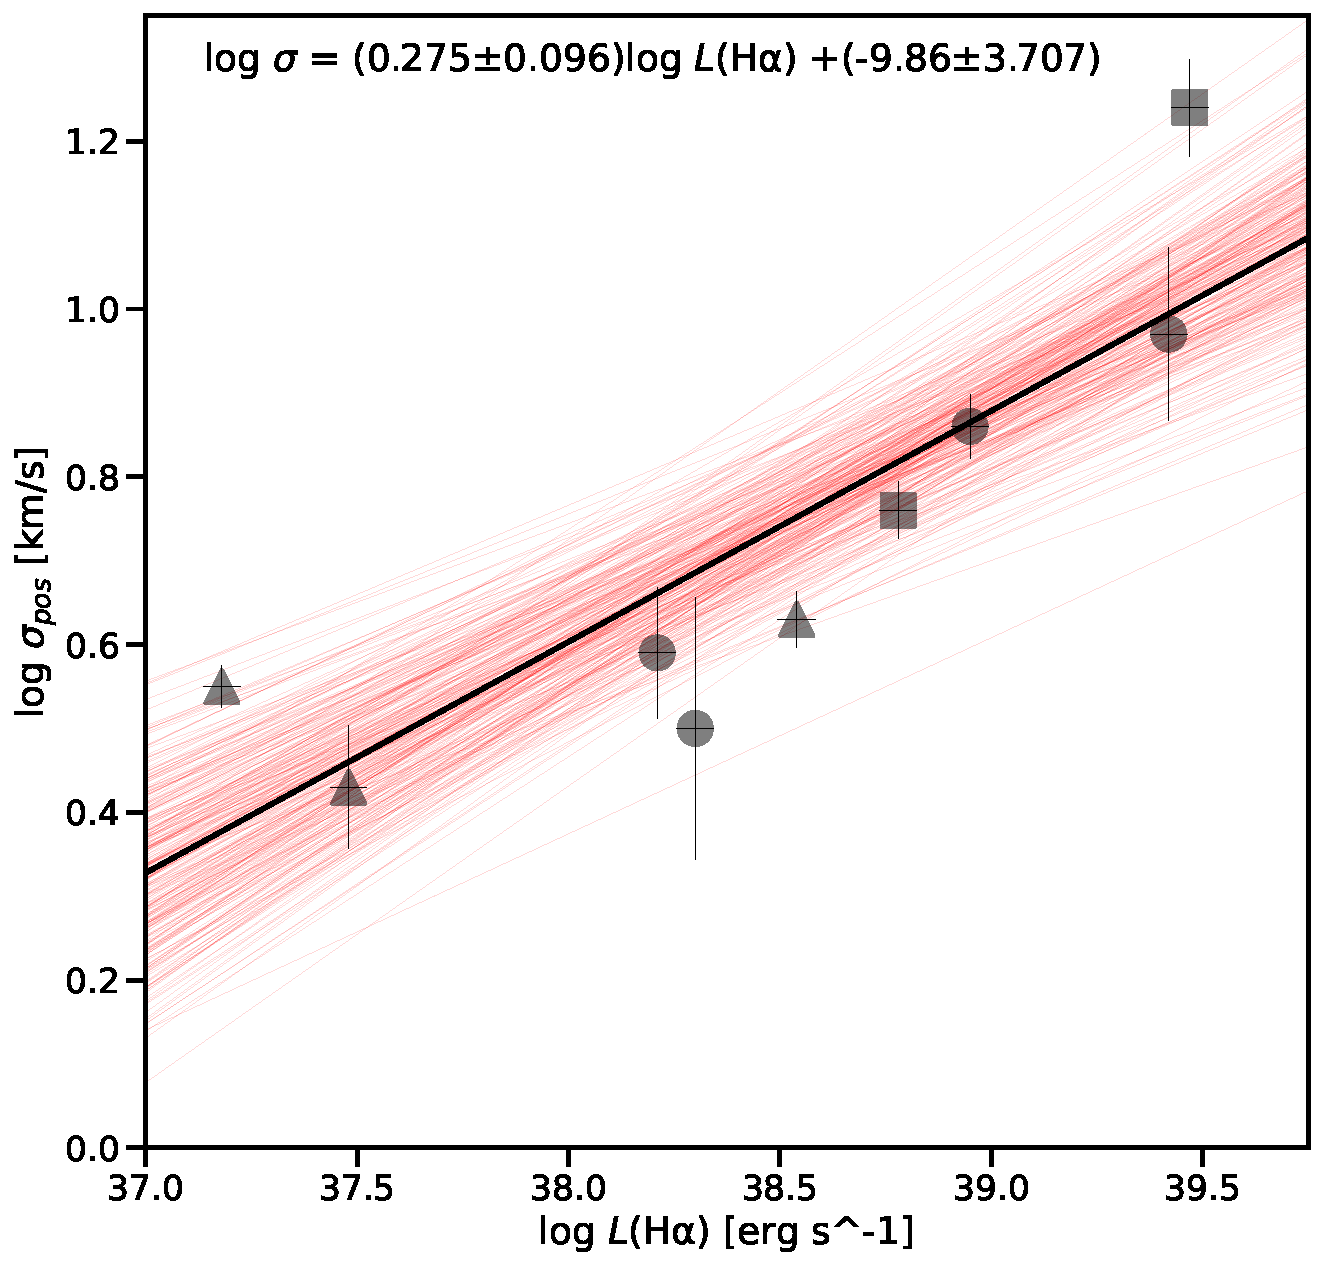
\includegraphics[width=3in]{Figures/corr-svsL}
\caption{
  The relationship between plane-of-sky velocity dispersion,
  \(\log_{10} \sigma\pos\),
  and \hii{} region luminosity,
  \(\log_{10} L(\ha)\),
  derived from our results.
  The markers indicates Galactic (triangles),
  Magellanic (squares) and extragalactic (circles) regions.
  The black solid line is the median linear regression,
  with thin red lines showing 400 random samples from the posterior
  distribution to indicate the uncertainty in the regression.}
\label{fig:sigvsl}
\end{figure}

\begin{figure}
\centering 
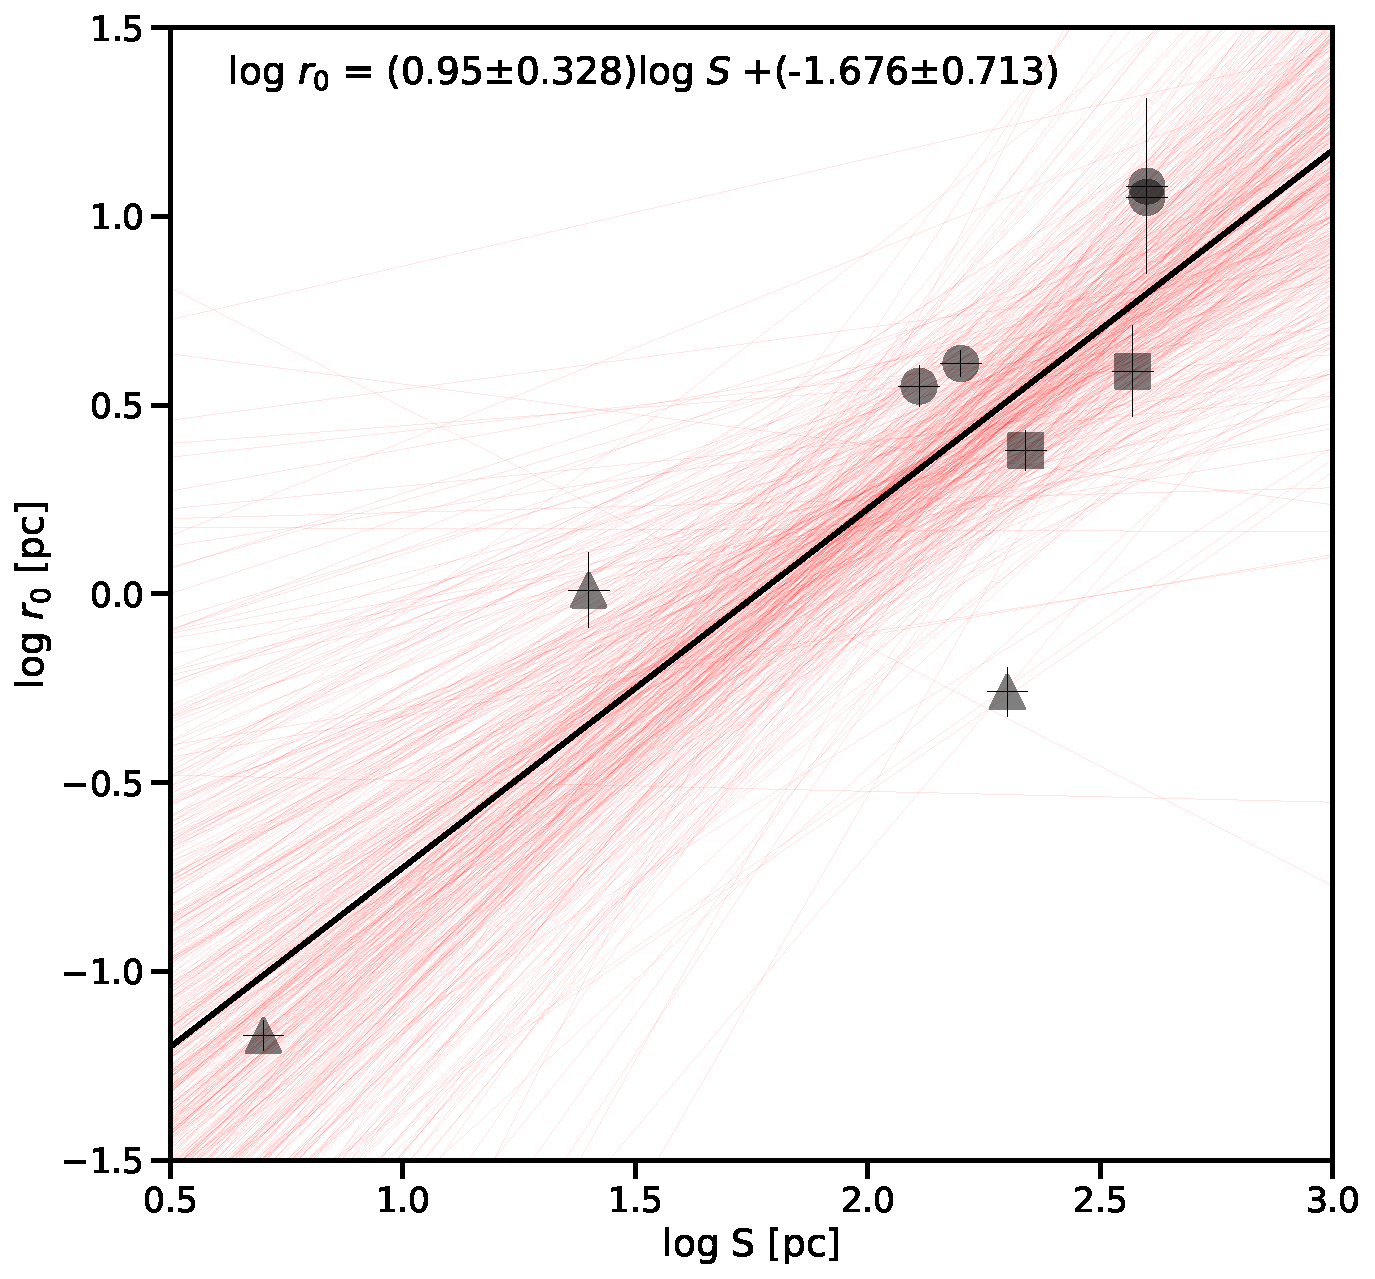
\includegraphics[width=3in]{Figures/corr-rvsS}
\caption{
  As Figure~\ref{fig:sigvsl} but for the relationship between
  correlation length of velocity fluctuations,
  \(\log_{10} r_0\),
  and  \hii{} region diameter,
  \(\log_{10} D_{\hii}\).}
\label{fig:rvsR}
\end{figure}

\begin{figure}
\centering 
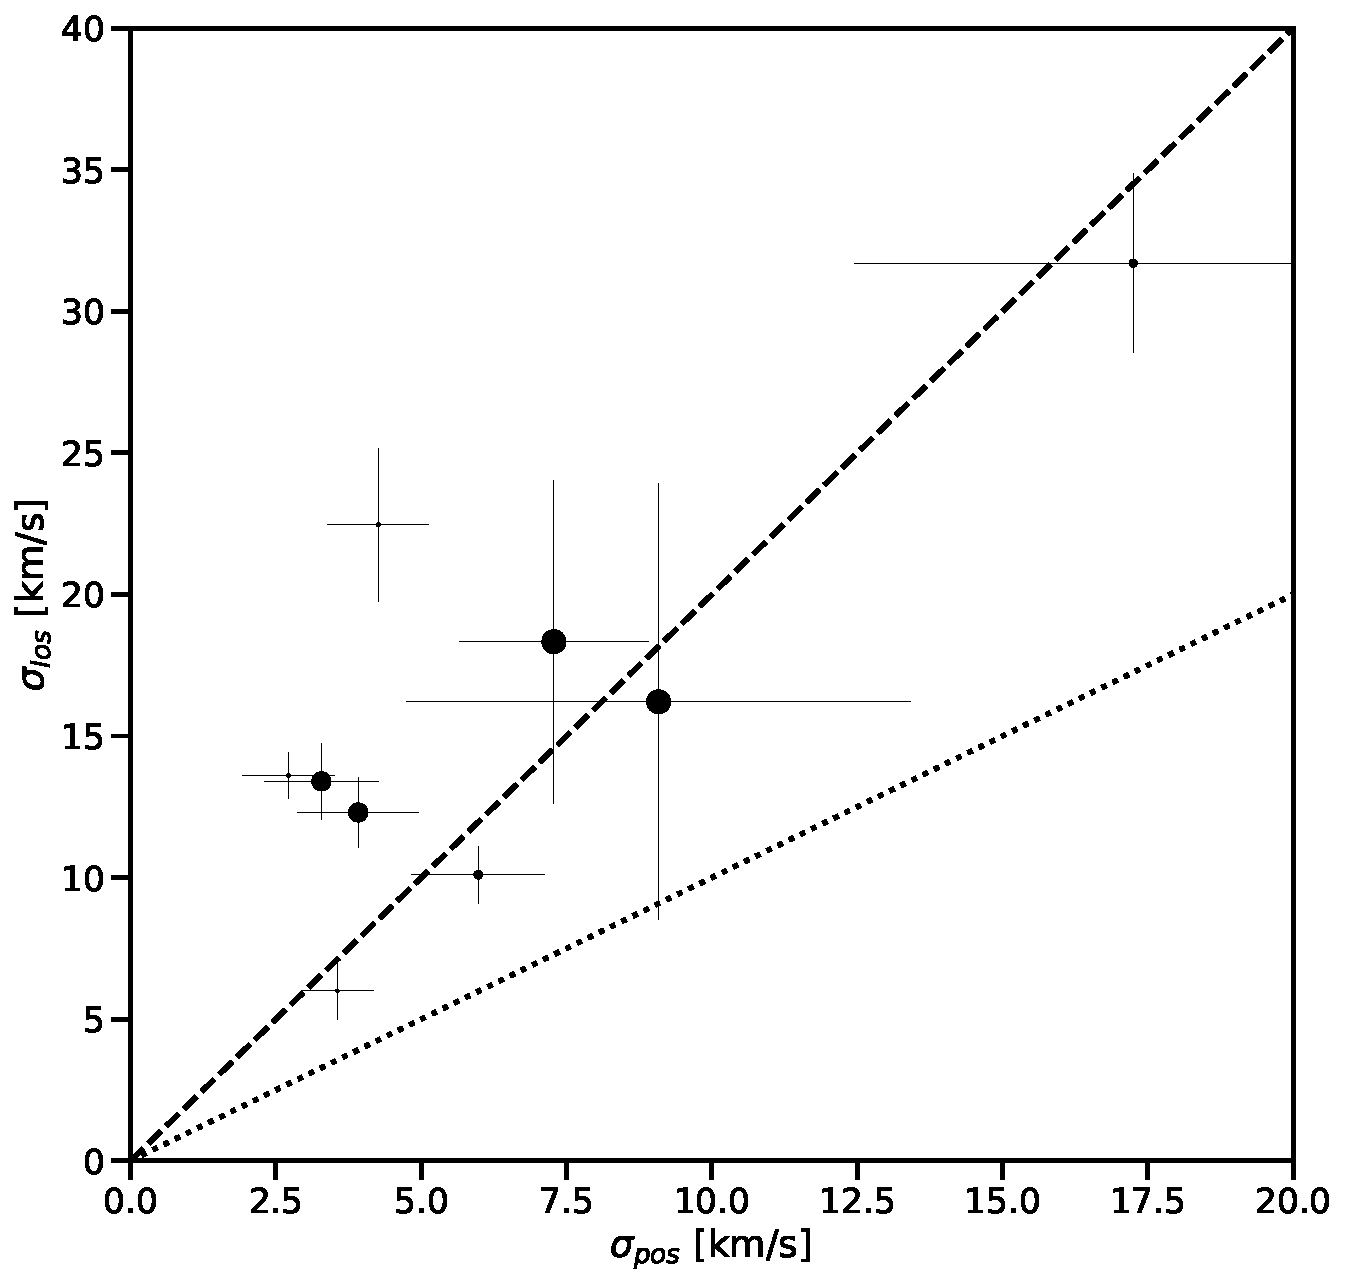
\includegraphics[width=3in]{Figures/corr-los-vs-pos}
\caption{
  As Figure~\ref{fig:sigvsl} but for the relationship between
  line-of-sight non-thermal velocity dispersion,
  \(\sigma\los\),
  and plane-of-sky velocity dispersion,
  \(\sigma\pos\).
  The dashed line shows the the linear fit obtained by
  \citet{2011MNRAS.413..705L} for a sample of
  small-to-intermediate size \hii{} regions in the M33 galaxy. 
}
\label{fig:los-vs-pos}
\end{figure}

\subsubsection{Luminosity vs centroid velocity dispersion}\label{sec:L-vs-sigmapos}

The Fig. \ref{fig:sigvsl} shows the log \(\sigma\pos\)-log \(\text{L}(\text{H}_{\alpha})\) plane.
This relation is commonly employ in the literature  and can be use to investigate how reliable is our derived velocity dispersion.
The fit we obtain is \(\log \sigma\pos = (0.27 \pm 0.10) \log \text{L}(\text{H}_{\alpha})-(9.9 \pm 4.0)\).
Since it is customary in the literature to present \(\text{L} (\text{H}_{\alpha})\) as the dependent variable we also calculate this relation: taking the inverse of slope in Fig. \ref{fig:sigvsl} we have \(\text{L}_{\text{H}_{\alpha}} \propto \sigma^{3.6 \pm 1.4}\) and using the same procedure in \textit{linmix} and changing the variables we obtain \(\log \text{L}(\text{H}_{\alpha}) = (2.8\pm 1.0) \log \sigma\pos -(36 \pm 4)\).

The relationship \(\text{L}_{\text{H}} \propto \sigma^{\alpha}\) has been extensively investigated  in the context of giants \hii{} regions obtaining a value for \(\alpha\) of \( \sim 4\)\citep{terlevich1981,1988A&A...201..199A} and \num{2.87 \pm 0.2} \citep{Rozas:2006b}.
Complementing previous results \citet{2012MNRAS.422.3339W} found that star-forming regions at \(z \sim 1.3\) and local \hii{} regions follow a relation with \(\alpha = 4.18 \pm 0.21\).
\citet{Moiseev:2015a} found that this relation also holds for dwarf galaxies with a value of \(\alpha \sim 5\).
\citet{2018MNRAS.474.1250F} presented the relationship between integrated H$_{\beta}$ line luminosity for new data of 36 giant HII regions obtaining \(\text{L}_{\text{H}_{\beta}} \propto \sigma^{5.02 \pm 0.21}\).
Recently, \citet{2020ApJ...888..113W} studied the properties of high-\(z\) and local \hii{} galaxies among some GEHRs findig a value of \(\alpha \sim 5\).

There are two main difference between the previous investigations and our results: one is that the velocity dispersion is obtained as the width of the emission line profile integrated over the whole object or as the non-thermal line-width, which is different from the plane of the sky dispersion we are using and that our sample is considerably smaller in the data points.
The first problem is addressed in section \ref{sec:sigmapos-vs-sigmalos} where we discuss the relation between the line-of-sight and plane-of-sky velocities.
But despite these problems, the fact that this relationship holds in our results (within the errors) is interesting considering that the \(\sigma\pos\) is derived from the structure function, while the \(\text{L}(\text{H}_{\alpha})\) values comes from different sources unrelated to our data (see the Appendix~\ref{sec:notes-individual-hii}).
This means that the proposed structure function model describes within certain accuracy the velocity field fluctuations and that the parameters obtained can be interpreted as a true kinematic property of the \hii{} region velocity field.

\subsubsection{Diameter vs correlation length}\label{sec:D-vs-r0}

The Figure \ref{fig:rvsR} shows the relation of the correlation length \(r_0\) and the diameter \(D\) of the region. 
The relationship we found is \(\log r_0 = (0.95 \pm 0.33) \log D - (1.6 \pm 0.7)\).
The values of \(D\) are taken from \citet{1984ApJ...287..116K} and correspond to the outer
limits seen from visual inspection of \ha{} photographs.
These values would represent an upper limit of the size of each region.
Since these objects do not posses physical edges the determination of their size is not trivial.
Due to the above, we chose these set values since they are from an unique source and are foreign to our calculations and observations, which reduced the bias in the scaling law we obtain.

Ideally the correlation length \(r_0\) should represent the scale of dominant energy injection.
It is unclear what are the precise mechanisms driving the turbulence in \hii{} regions.
There are several energy sources that could provide or contribute to the energy required: of the order of kpc we have the differential rotations of the galaxy that produces shear at large scale. 
At scales of the order of hundreds of pc the supernova explosions inject a large amount of kinetic energy.
At scales of several tens of pc the expansion of \hii{} regions and stellar winds are a source of energy, and bipolar flows, shocks, jets and champagne flows inject energy at small scales about one tenth of a pc.
Many of these mechanisms, at some extent, affect all the \hii{} regions studied in this work, so the most probable scenario is that the velocity fluctuations are consequence of the combination of various mechanism.

The dependence on \(r_0\) and the diameter can be interpreted in terms that each region presents a characteristic energy injection mechanism (or combination) and despite the presence of the different mechanisms there is some unique combination that drives the input energy in each region. 

\subsubsection{Relationship between plane-of-sky and mean line-of-sight velocity dispersion}\label{sec:sigmapos-vs-sigmalos}

The second-order structure function measures the velocity fluctuations in the \hii{} regions under the assumption that there exists an underlying velocity spectrum following an energy cascade.
But this statistical technique is not unique in measuring the velocity fluctuations in the nebula.
Two parameters which can be obtained from the velocity profile also measure the velocity fluctuations in the \hii{} regions: the standard deviation of the velocity centroids, \(\sigma\pos\), and the mean non-thermal linewidth, \(\langle \sigma_{\text{los}} \rangle\).
These quantities allow us to compare the relationship between the kinematical disorder on the plane-of-the-sky and along the line-of-sight \citep{2011MNRAS.413..705L,arthur2016turbulence}.

The \( \sigma_{\text{los}} \) parameter is estimated by correcting the observed linewidth for the contribution of broadening mechanism, equation \eqref{eq:sigma-los}, leaving just the random motions which are interpreted as random motions along the line-of-sigth.
This method is a simplification of the problem since it assume a Gaussian profile fit, which does not consider other components that could arise from different kinematics processes of the ionized gas and leaves out the broadening due to dust scattering \citep{castaneda1988,1998ApJ...503..760H}.

In the Fig.~\ref{fig:los-vs-pos} we show the mean line-of-sight velocity dispersion versus the plane-of-sky velocity dispersion plane.
The relationship we obtain is \( \langle \sigma\los \rangle = (1.03 \pm 0.46) \sigma\pos + (7.7 \pm 2.9)\).
\citet{arthur2016turbulence} presents the same diagram for different emission lines of the Orion core nebula showing that the value \(\sigma_{\text{los}}\) (after considering the dust scattering) is roughly twice as the \(\sigma\pos\) (figure 14 on their work), while the \citet{2011MNRAS.413..705L} diagram, for a sample of small-to-intermediate size \hii{} regions in M33, approach unity (figure 4 on their work) with a linear relation of \(\langle \sigma_{\text{los}} \rangle = (1.04 \pm 0.14) \sigma\pos + (8.15 \pm 0.93) \).

As for the interpretation, it is possible to consider that large fluctuations of the turbulent velocities, which are spread over the entire ionized extent of the nebula, increase monotonically with the plane-of-sky dispersion.
In this scenario, the main broadening mechanisms causing kinematical disorder along the line-of-sight are related to the velocity gradients of the clumpiness in the cloud and turbulent movements.
On the plane-of-sky the consequences of those gradients and movements are measured in every pixel, consequently the spatial variations on the velocity field would depend on the targeted pixel, at the same time depending on the motions inside the cloud.
Thus the \(\sigma\pos\) and \(\langle \sigma_{\text{los}} \rangle\) parameters increase in the same amount as the fluctuations grows \citep{2011MNRAS.413..705L}.

The case of the reduction in the \(\sigma\pos\) can be interpreted by the effect of \textit{project smearing} \citep{1984ApJ...277..556S}.
If we consider the case of homogeneous turbulent velocity, the projection from three to two dimensions over the line-of-sight depth \(H\), reduces the plane-of-sky amplitude for the condition \(r_{0} < H\).
With a value of \(\sigma\pos / \sigma_{\text{los}}\) = 0.5 we obtain \(r_{0} / H \sim\) 0.02 - 0.1.
This procedure implies depths of the order 10 to 50 times the correlation length.
In the lower limit \citet{arthur2016turbulence} mentioned the inconsistency of this interpretation for the Orion core nebula, since evidence has shown that the emitting layer thickness is of the order of \num{0.01} - \SI{0.3}{pc}.
%For the most distant regions of our sample, the previous analysis would give depths of the order of magnitude of the observational box, but considering the analysis using the power-law index (see section~\ref{sec:power-index}) only NGC 595, which power-law index is \num{1.38}, would comply to this fully three-dimensional structure.
On the other hand, \citet{arthur2016turbulence} proposed another interpretation in terms of large-scale order motions, and emissivity fluctuations.
They consider an expanding shell where the mean velocity fluctuations on the plane of the sky are because the relative brightness of the redshifted and blueshifted hemispherers.
In this case, the rms fractional variation in the emissivity on the scale diameter is found to be in the order of \(\sigma\pos / \sigma_{\text{los}}\) ratio.


\subsubsection{Diameter vs centroid velocity dispersion}

Other important relationship commonly used in the study of the interstellar medium is the diameter (or size) versus velocity dispersion.
Table \ref{tab:RestStats} shows this result for our sample in the forth row. 
This relation presents a significance level \(p > \num{0.05}\) but there are a couple of things worth mentioning.
Historically this relation is important following the work of \citet{1981MNRAS.194..809L} where he presents it in the context of molecular cloud complexes of many clouds, individual clouds, and clumps, so that size scales are studied over \(\num{0.1} < L < \SI{100}{pc}\) obtaining \(\sigma = 1.10 L ^{0.38}\). 

This relation is interpreted in terms of turbulence, particularly the Kolmogorov model which predicts a index of \num{0.33} so that larger regions presents more turbulence, and smaller regions less turbulence.
It has been argued that this correlation method is not as powerful as using statistical functions \citep{1984ApJ...277..556S} but it is interesting that the index is consistent within different phases of the interstellar medium.
We obtain \(\log \sigma\pos = (0.25 \pm 0.17) \log D - (0.2 \pm 0.38)\) which is comparable with \citet{1981MNRAS.194..809L} results.

As we mentioned in section \ref{sec:L-vs-sigmapos} the fact that this relation holds up to previous investigation gives some certainty that the \(\sigma\pos\) value obtained via the proposed model of the structure function is valid. 
This implying that the structure function, while not an absolute diagnostic, is a powerful tool in the research of \hii{} regions kinematics.

\subsection{Power-law index}\label{power-law-index}

The power-law index \(m\) shown in the last column of Table \ref{tab:Res} is used for comparison between the observations derived index and the theoretical Kolmogorov value of 0.67.
All our indices are above this theoretical value and this is attributed to the fact that the \hii{} regions do not comply with the conditions established in the development of the turbulent theory which assumes incompressible, subsonic and homogeneous three-dimensional flow.
\hii{} regions emerged from a molecular cloud with highly filamentary and clumpy density structure.
Inside the region there is a large increase in the temperature because of the photoionization, and the density gradients with the pressure gradients accelerate the flow which occurs on multiple scales consequence of the fractal nature of the molecular cloud \citep{arthur2016turbulence}.
The radiation pressure, stellar winds and region expansion, among other physical processes would create pressure-driven shock waves propagating faster than the speed of sound in the medium.
This would make the flow compressible and supersonic in an inhomogenous gas cloud.
Also, as \hii{} regions are three-dimensional objects our structure function results comes from a projection of this three-dimensional structure to a two-dimensional velocity field.
But despite the complex nature of \hii{} regions and observational limitations, we obtain a common pattern for the structure function behaviour and the value of the power-law index falls in a certain limited range between \num{0.7} and \num{1.4}. 

The differences in the power-law index with respect the theoretical value are often used as a diagnostic tools to identify properties that are not consider in the assumptions of the turbulence theory \citetext{See table~1 of \citealp{arthur2016turbulence} and Sec.~1 of \citealp{lagrois2011}}.
As an example there the so called \textit{projection smoothing} \citep{von1951methode,1987ApJ...317..686O} which is used to study the projection of a three-dimensional structure function on the plane.
The relationships for the power-law are:

\begin{equation}\label{eq:projection-smoothing-3d}
m_{2D}= m_{3D} + 1
\end{equation}
%
and  when the astronomical object present a sheet-like distribution of emitters we have the relation:
%
\begin{equation}\label{eq:projection-smoothing-2d}
m_{2D} \sim m_{3D}
\end{equation}

As a conclusion, if the extension of the HII region is compared with its depth (three-dimensional case) the value of the index is \num{1.6}. 
While the case where the extension is much greater than its depth (two-dimensional case) the region will have a value of \num{0.6}.
From Table~\ref{tab:Res} we see that our results fall between these two previous values. 

As for any relation of the power-law index \(m\) and the physical properties of the \hii{} regions we can see from table \ref{tab:RestStats} that this parameter does not correlate with any other parameter or physical property, being the least reliable for determining or concluding something about the nature of the physical processes inside the regions.
On the other hand, the lack of correlation and the presence of this power-law index describing the assumed energy cascade may be interpreted as a universal property of the velocity fluctuations independent of the observed object, which is the main consideration in the turbulence theory.

 
%\subsection{Kinematic relationship between ionized gas, molecular gas, and stars}
%\label{sec:kinem-rela-betw}

%Naively, the relatively small observed CO velocity dispersion
%(\(\sigma(\chem{CO}) \ll \sigma(\ha)\) in all regions
%for both \(\sigma\los\) and \(\sigma\pos\))
%might be thought to rule out the molecular gas kinematics
%as a \emph{cause} of the ionized gas kinematics.
%However, this is not necessarily the case, so long as \emph{some} molecular gas
%exists at the higher velocities typical of the ionized gas.

%This is because a relatively small column of material
%(\(N(\chem{H}) \sim \SI{e20}{cm^{-2}}\))
%is sufficient to trap the ionization front,
%in which case the \ha{} surface brightness is limited by the
%incident ionizing flux
%\citetext{the Ferland mechanism,
%  see section~5.1 of \citealt{Baldwin:1991a}
%  and section~B.2.1 of \citealt{Ferland:2012a}
%}.
%On the other hand, the bulk of the CO emission will come from much larger
%column densities (\(N(\chem{H}) \sim \SI{e22}{cm^{-2}}\)),
%where the molecules are effectively shielded from dissociation.
% If a given region can be considered as an ensemble of clouds of
% different masses, then ... would require lower mass clouds to move
% faster though, so needs dynamical relaxation

%\textbf{Check  if this is actually feasible before developing further}

%Very schematically, one could represent these processes as:
%\begin{equation}
%  \label{eq:1}
%  \sigma^2(\ha) \sim \zeta \sigma^2(\chem{CO}) + \eta
%\end{equation}
%where \(\zeta\) is a multiplicative factor
%due primarily to the saturation at the Ferland limit,
%and \(\eta \sim \csound^2\) is an additive factor due to additional turbulence
%generated by the transonic ionized photoevaporation flows.

%\textbf{Estimate these two factors by fitting to the observations}

%\subsection{Interpretation of the turbulent parameters}\label{sec:interpretation-parameters}

%\subsubsection{Correlation length \(r_0\)}

%Ideally the correlation length \(r_0\) should represent the scale of dominant energy injection.
%It is unclear what are the precise mechanisms driving the turbulence in \hii{} regions, thought a lot of options are candidates.
%The most probable scenario is that the velocity fluctuations are consequence of the combination of various mechanism.
%There are several energy sources that could provide or contribute  to the energy required: of the order of kpc, the differential rotations of the galaxy that produces shear at large scale, at scales of the order of hundreds of pc, supernova explosions inject a large amount of kinetic energy.
%At scales of several tens of pc the expansion of \hii{} regions and stellar winds are a source of energy and, bipolar flows, shocks, jets and champagne flows inject energy at small scales about one tenth of a pc.
%Many of these mechanisms, at some extent, affect all the \hii{} regions studied in this work.
%We can use the kinematic analysis of the regions to investigate how previously identified energy injection mechanisms could be related to the correlation length. 

%\citet{2009AJ....137..367O} present a three-dimensional study of the dynamic structure of the Orion nebula.
%The high-velocity stellar wind from \(\theta^1\) Ori C will confine the ionized gas, even the high ionization emission lines, to a thick shell.
%In one direction, at a distance of \SI{0.1}{pc} from the ionizing massive star a stationary shell of shocked material is formed when the ram pressure of the photoevaportation flow balances the thermal pressure of the shocked wind.
%In the other direction there is a free flow of the hypersonic wind.
%At a smaller scale of \SI{0.02}{pc} there is an interaction between the closest proplyd photoevaporation flow and the stellar wind which results in bowshocks.
%According to \citet{2001ApJ...561..830G} the influence of stellar wind interactions is restricted to the central \SI{0.05}{pc}. 
%Orion also present a champagne flow where the photoionized gas streams away from the ionization front covering a distance of \SI{\sim 1}{pc} from the molecular cloud \citep{1973ApJ...183..863Z}.

%Our correlation length results for the Orion Core and EON from table~\ref{tab:Res}, \num{0.068} y \SI{0.39}{pc} respectively, despite been of the order of the scales mentioned above still aren't conclusive enough to determine a direct relation between them.
%As mentioned in \citet{arthur2016turbulence} the mechanism mentioned in the previous paragraph would play a secondary role in stirring up the gas motions and it would be necessary to specify if the velocity fluctuations arise from pure turbulent motion inside the ionized clouds or a consequences of density and brightness fluctuations.

%\citet{sabalisck1995supersonic} studied NGC 604 revealing that the high emission knots on the region encompasses supersonic global velocity dispersion values of 14 $<$ \(\sigma_{\text{los}}\) $<$ \SI{20}{km.s^{-1}}.
%This knots have a characteristic radius of \(\sim\)\SI{7}{pc} and a Gaussian profile.
%Values of velocity dispersion $>$\SI{20}{km.s^{-1}} are found in low emission cavities where the lines present strong asymmetries.
%These cavities were identified as expanding shells by \cite{yang1996} with diameters of \(\sim\)\SI{40}{pc} and a expansion velocity above \SI{50}{km.s^{-1}}.
%According to table~\ref{tab:Res} the correlation length for NGC 604 is close to the scale of the bright knots in the region which aren't related to a particular energy injection mechanism.

%Although the Orion core, the EON, and NGC 604 have different \(r_0\) is not clear if it truly %reveal a concrete aspect of the energy input mechanism mentioned above.
%Orion main energy input comes from one star, meanwhile NGC 604 has more than 200 OB stars including WR stars. 
%The Orion core also presents Herbig-Haro objects, which aren't possible to resolve for more distant regions.
%Though the correlation length is particular to each region, and it is correlated mainly with the size (see section~\ref{sec:scaling-relations}), it still needs further studies to reveal the true implication of this value with respect the energy input mechanisms.

%\subsubsection{Structure function power-law index \(m\)}\label{sec:power-index}

%The index \(m\) shown in the last column of Table \ref{tab:Res} is used for comparison between observations and the theoretical value of 0.67.
%All our indices are above this theoretical value and this is attributed to the fact that the \hii{} regions do not comply with the assumptions established in the development of the turbulent theory.

%From section~\ref{sec:regions-milky-way} we know that most of all assumption mentioned in the theory of turbulence are not meet for our \hii{} region sample.
%\hii{} regions emerged from a molecular cloud with highly filamentary and clumpy density structure .
%There is a large increase in the temperature because of the photoionization, and the density gradients with the pressure gradients accelerate the flow which occurs on multiple scales consequence of the fractal nature of the molecular cloud \citep{arthur2016turbulence}.
%The radiation pressure, stellar winds and region expansion, among other physical processes would create pressure-driven shock waves propagating faster than the speed of sound in the medium.
%This would make the flow compressible and supersonic in \hii{} regions.
%Also, as \hii{} regions are three-dimensional objects our structure function results comes from a projection of this three-dimensional structure to a two-dimensional velocity field.
%But despite the complex nature of \hii{} regions and observational limitations we obtain a common pattern for the structure function and the value of the power-law index falls in a certain limited range of values. 
%The differences in the power-law index with respect the theoretical value are often used as a diagnostic tools to identify properties that are not consider in the assumptions of the turbulence theory.

%To study the projection of a three-dimensional structure function to a two-dimensional structure function, known as projection smoothing \citep{von1951methode, munch1958internal,1964SvA.....8..210K,1987ApJ...317..686O}, relationships between the power-law indices were proposed:

%\begin{equation}\label{eq:projection-smoothing-3d}
%m_{2D}= m_{3D} + 1
%\end{equation}
%
%and  when the astronomical object present a sheet-like distribution of emitters we have the relation:
%
%\begin{equation}\label{eq:projection-smoothing-2d}
%m_{2D} \sim m_{3D}
%\end{equation}

%As a conclusion, if the extension of the HII region is compared with its depth (three-dimensional case) the value of the index is \num{1.67}. 
%While the case where the extension is much greater than its depth (two-dimensional case) the region will have a value of \num{0.6}.
%From Table~\ref{tab:Res} we see that our results fall between these two previous values. 

%The mean value \(m\) of our sample is \num{\sim 1}. 
%Following the equation \ref{eq:projection-smoothing-3d} the \hii{} regions in our sample with \(m >\) 1 would present a depth which is in the order of magnitude comparable to the length of %the observed box size \(L\) been closest to this value as \(m\) tends to 1.6. 
%On the other hand, \hii{} regions with values \(m <\) 1 would present a thinner structure as they tend to the value of 0.6.
%This analysis should not be regarded as conclusive about the true structure of the regions and would require further observations with a combination of kinematics analysis to determine the best way to determine the depth of each region.
%%%%%%%%%%%%%%%%%%%%%%%%%%%%%%%%%%%%%%%%%%%%%%%%%%%%%%%%%%%%%%%%%%%%%%%%%%%%%%%%%%%%%%%%%%%%%%%%%%%%%%%%%%%%%%%%%%%%%%

\section{Conclusions}\label{sec:conclusions}

%The observations point out to the existence of spatial correlation between velocities, that could be interpreted as turbulence. 
%Arguments against the existence of true, isotropic turbulence can be raised as, for example: i) the histograms of velocity are not always Gaussian, ii) only a fraction of the integrated emission lines of the \hii{} regions show true Gaussian profiles. 
%The asymmetry in the emission line indicates coherent mass flow motions, 
%and sometimes is considered incompatible with turbulence. However, turbulence is in fact 
%a mixture of coherent and chaotic flows. 
%Only at the regime of the so-called fully developed turbulence the non-linear phenomena dominate completely the movement and the chaotic flow prevail. 
%The problem here is that a straightforward test for any turbulent model is a big challenge, as we are in the presence of many entangled effects. 
%However, the circumstantial evidence in favor of the existence of turbulent motions in \hii{} regions is overwhelming, and many are the potential sources of energy to create and maintain turbulence during the lifetime of an \hii{} region.

Our analysis was able to characterize the velocity fields of a sample of \hii{} regions by determining a set of parameters unique to each velocity field which are: the correlation length, the exponent of a power law that fits the results through a determined range and the true velocity dispersion.
To achieve this, a new functional form for the second-order structure function was proposed. 
This new functional considers observational constraints such as the seeing, noise and the size of the observational box, effects that had not been considered before and play an important part in the interpretation of the structure function.
Our proposed functional form is used as an objective function in a non-linear regression to accurately determine the set of parameters related to turbulence and to the observational constraints.

The observed structure functions calculated in our work does not reveal the precise characteristic of turbulence, but the statistical results that it provides allow us to determine a distinction between correlated or random velocity fluctuations in the photoionized gas, in which the presence of correlations in the velocity field is a inherent property of turbulence.
Although this work is not conclusive about the nature of photoionized gas turbulence and a precise description of the origin and implications of these turbulent motions is out of the scope of our investigation, we believe that the tools presented here (see section~\ref{sec:methods-apply}) guarantee a more realistic approach to determine and to the understanding the structure function.

Our analysis can be easily be expanded to other \hii{} regions with the possibility of comparing the results between them since our method guarantees homogeneity, providing the possibility to develop a future catalog of \hii{} regions turbulent parameters in a concise way.
By calculating the structure function of HII regions with different morphologies, ages, stellar content, and dynamics it would be possible to detect the presence and the importance of different sources of mechanical energy, since the structure function would be different from one object to the other as we show in the present investigation. 

Our methods could also been use to investigate the velocity fields of other phases of the interstellar medium.
The study of turbulence between ionized regions and the molecular clouds that give them birth can be carried out with the aid of a correct methodology with the intention of advancing the understanding of the kinematic relationships between them.



%%%%%%%%%%%%%%%%%%%%%%%%%%%%%%%%%%%%%%%%%%%%%%%%%%%%%%%%%%%%%%%%%%%%%%%%%%%%%%%%%%%%%%%%%%%%%%%%%%%%%%

\section*{Acknowledgements}

Based on observations made with KPNO telescopes
\textit{complete KPNO acknowledgment}.
Based on observations made with ESO Telescopes at the La Silla Paranal Observatory under programme IDs 076.C-0888 and 098.D-0211.
Based on observations made as part of the Gaia-ESO Spectroscopic Survey
\textit{complete Gaia-ESO acknowledgment}.
Based on observations made with the WHT
\textit{complete WHT acknowledgment}.
We are grateful to Norberto Castro Rodríguez for providing maps of emission line velocity moments for 30 Doradus derived from MUSE-VLT observations.
JGV acknowledges and thanks CONACyT-Mexico for the PhD research scholarship.

%%%%%%%%%%%%%%%%%%%%%%%%%%%%%%%%%%%%%%%%%%%%%%%%%%
%%%%%%%%%%%%%%%%%%%% REFERENCES %%%%%%%%%%%%%%%%%%

\bibliographystyle{mnras}
\bibliography{bibphd}

%\clearpage

%%%%%%%%%%%%%%%%%%%%%%%%%%%%%%%%%%%%%%%%%%%%%%%%%%
%%%%%%%%%%%%%%%%% APPENDICES %%%%%%%%%%%%%%%%%%%%%
%%%%%%%%%%%%%%%%%%%%%%%%%%%%%%%%%%%%%%%%%%%%%%%%%%

\appendix

\section{Degradation of the structure function due to observational limitations}
\label{sec:degr-struct-funct}
Studied in context of \(\Delta\)-variance by \citet{Bensch:2001l}.

To characterize the impact of the observational box size and the atmospheric seeing on the structure function we perform a series of experiments using artificial turbulent velocity maps.
We quantify how these observational limitations affect the determination of astrophysical interest parameters such as the correlation length \(r_0\) and the velocity field variance \(\sigma\pos^2 \). 
The artificial velocity maps are created using a modified version of the \textit{make$\_$extend} command from the \texttt{turbustat} Python library \citep{Koch2019AJ....158....1K}.
The modification add a tapering to the power law so that the generated fields are uncorrelated at large scales.
The artificial fields follows a given power law with with a correlation length giving a variance value indicated as true \(\sigma^2\).
Using this true \(\sigma^2\) we obtain the true \(r_0\) and these values are used as a reference in the experiments to quantify the variations.

\subsection{Finite box effects}
\label{sec:finite-box-effects}

\begin{figure}
  \begin{tabular}{@{} l @{}}
    (a)\\
    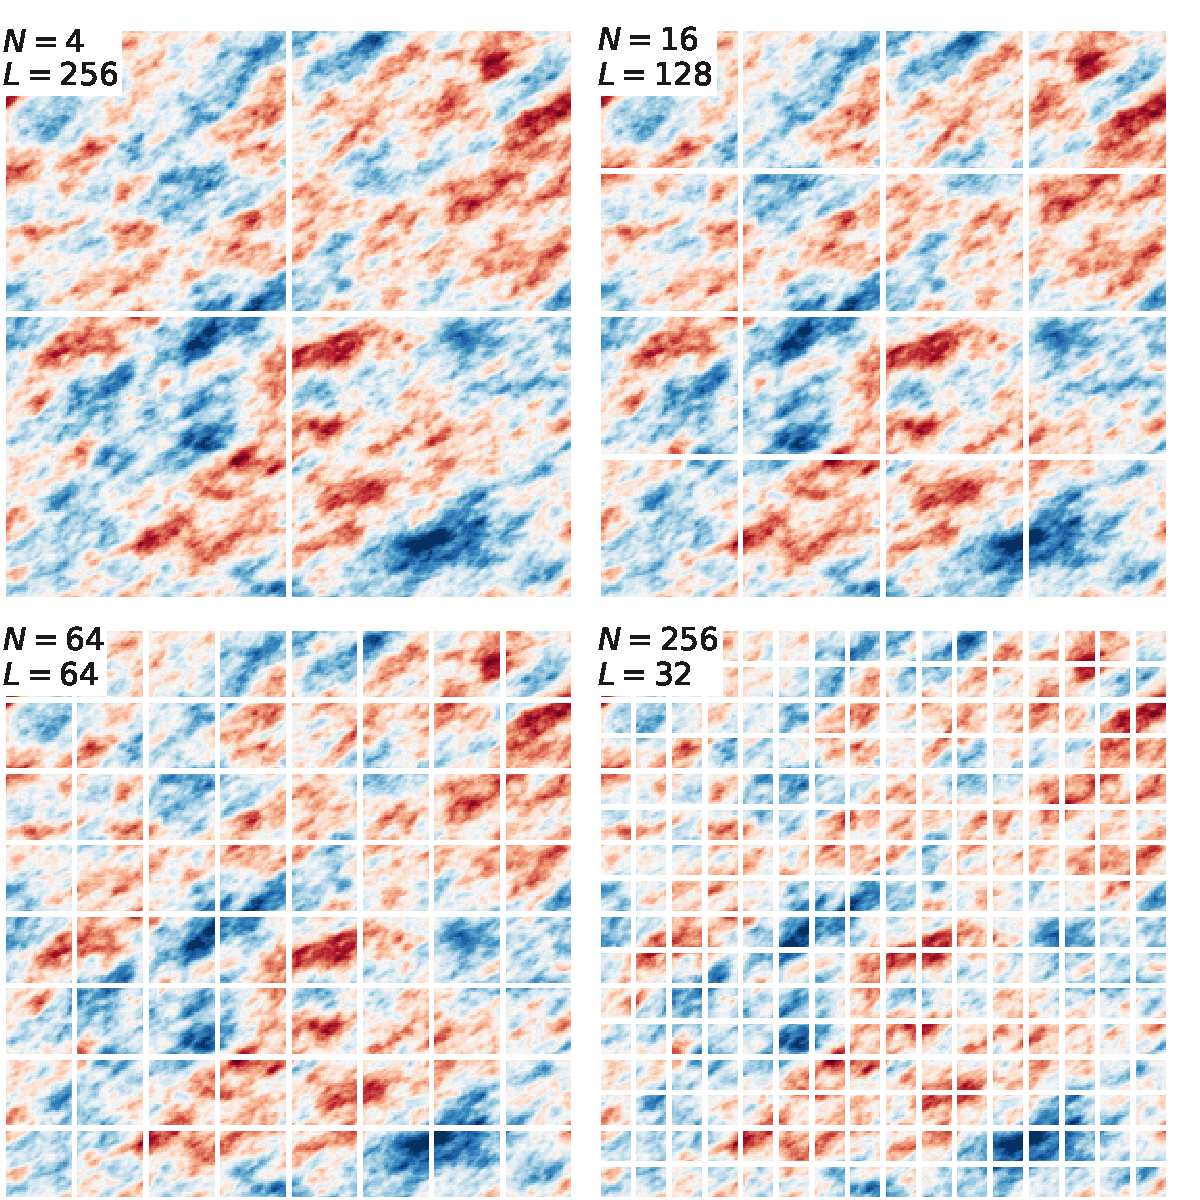
\includegraphics[width=\linewidth]{Figures/fake-finite-box-images}
    \\[\bigskipamount]
    (b)\\
    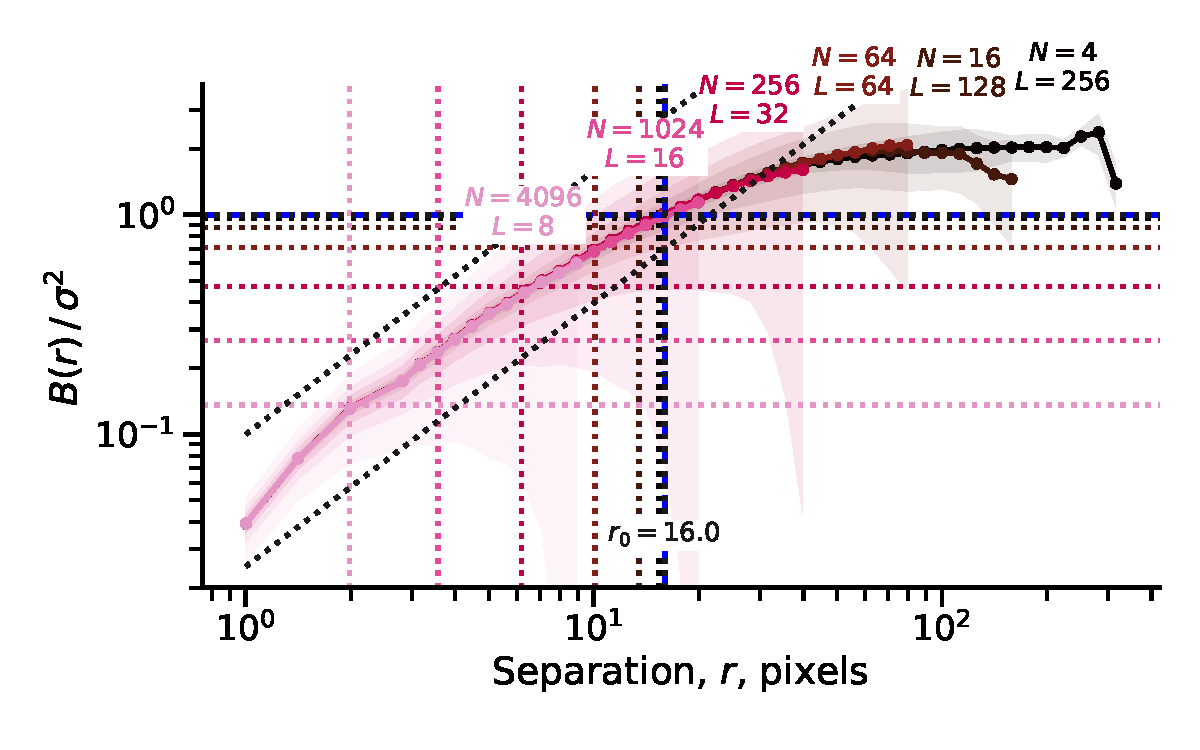
\includegraphics[width=\linewidth]{Figures/fake-finite-box-strucfunc2}
  \end{tabular}
  \caption{Effects of finite box size on the structure function.
    (a)~Construction of simulated turbulent velocity fields of different sizes
    by repeated division of an initial field of size \(512 \times 512\) pixels.
    The \(j\)th level of division yields \(N = 4^j\) fields,
    each of linear size \(L \times L\) where \(L = 2^{9 - j}\).
    The color scale is the same for all maps and it considers \(- 3\) to \(+ 3\) times the standard deviation.
    (b)~Resultant structure functions.
    Colored lines show the average \(B(r)\) over all sub-images,
    while the shaded areas show the standard deviation of \(B(r)\).
  }
  \label{fig:finite-box}
\end{figure}

\begin{figure}
  \begin{tabular}{@{} l @{}}
    (a)\\
    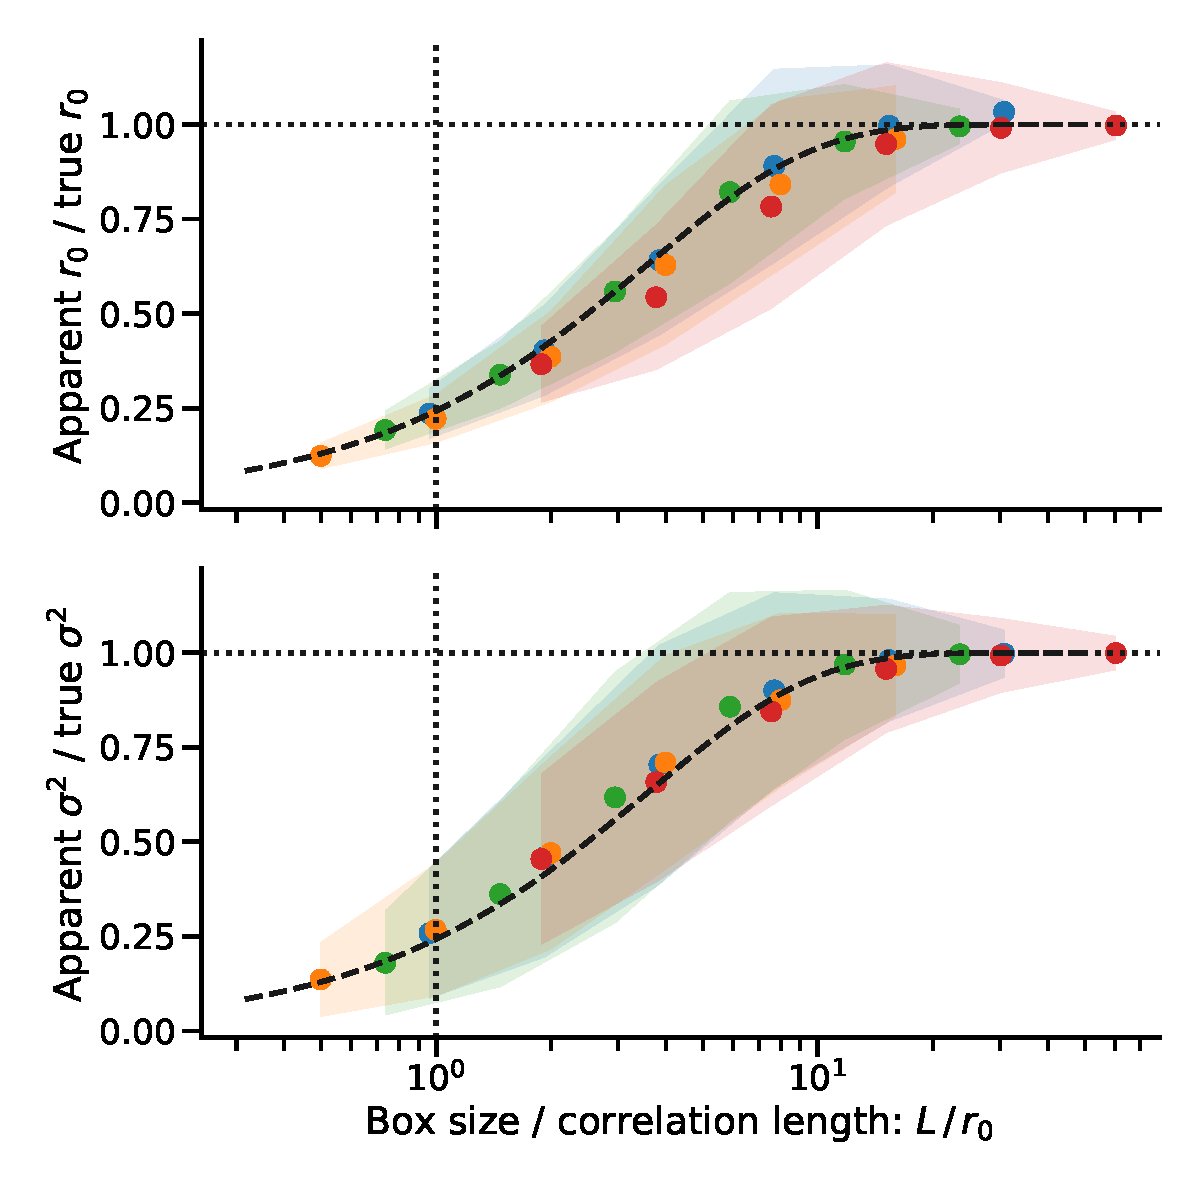
\includegraphics[width=0.95\linewidth]{Figures/fake-finite-box-effect}
    \\[\bigskipamount]
    (b)\\
    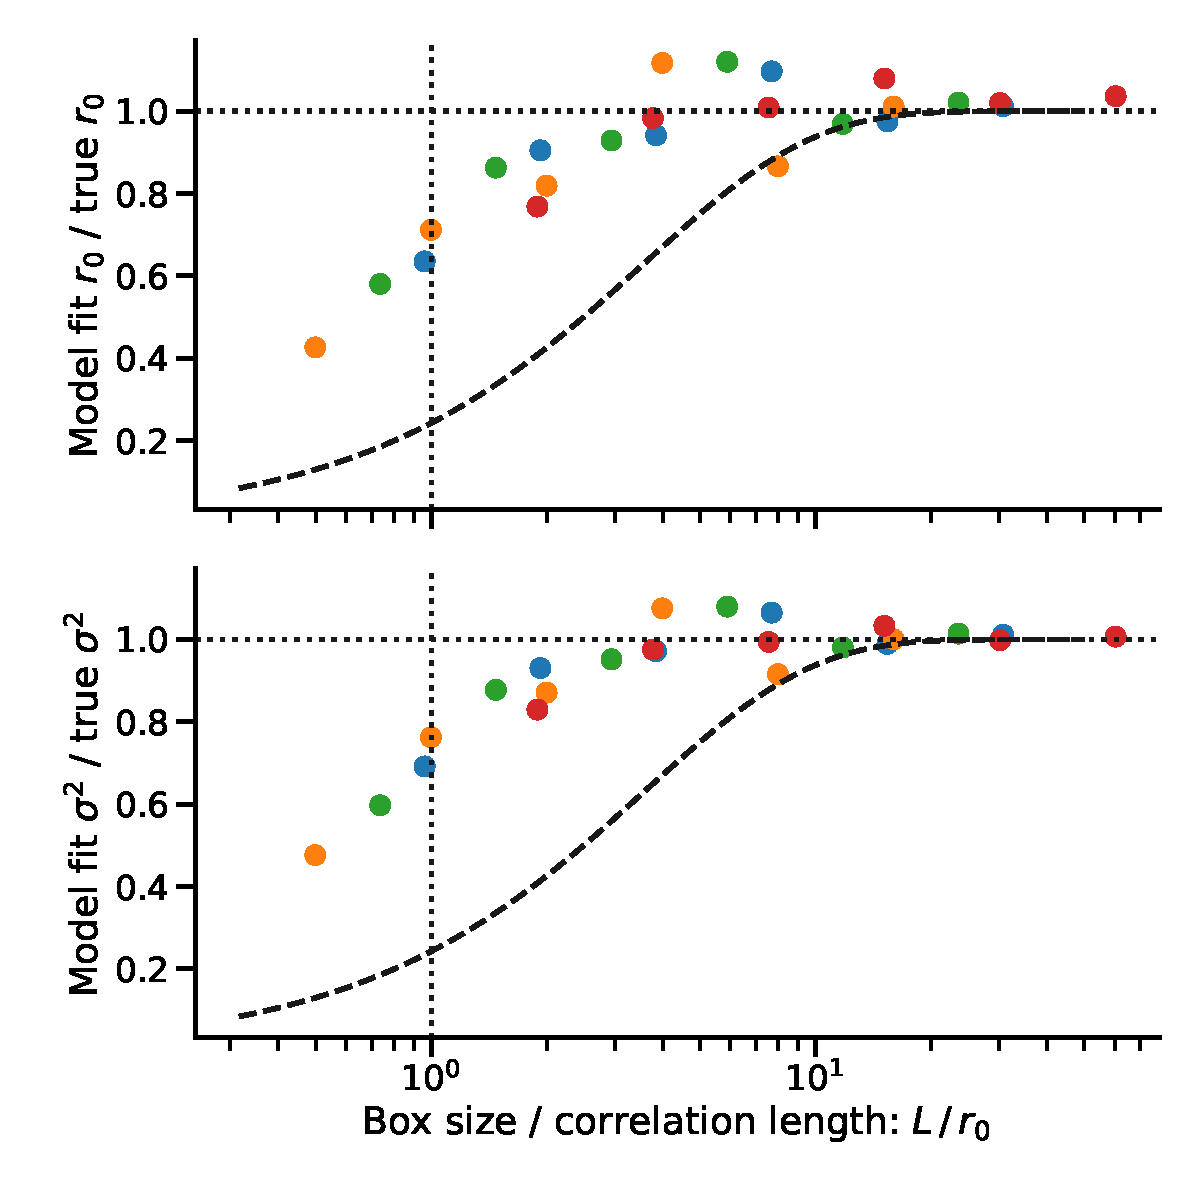
\includegraphics[width=0.95\linewidth]{Figures/fake-finite-box-fits}
  \end{tabular}
  \caption{
    Reduction of apparent velocity variance and correlation length
    due to finite box size.
    (a)~Empirical measurements of \(\sigma^2\) and \(r_0\).
    Colored dots show mean results from different simulated velocity fields,
    with different power law slopes.
    Colored shading shows the inter-quartile range over the different sub-images.
    The dashed line is an approximate analytic fit to these results
    (equation~\eqref{eq:ajustebox}).
    (b)~Determination of \(\sigma^2\) and \(r_0\) from fitting the model
    of equation~\eqref{eq:new-correlation-form}.
    Colored dots are mean results from different simulated velocity fields,
    while the dashed line is the same as in (a).
  }
  \label{fig:finite-box-effect}
\end{figure}

The Fig. \ref{fig:finite-box}a shows some of the artificial velocity fields used to study the variations in the structure function with respect to the size of the observational box.
Initially we have a velocity field of \(512 \times 512 \) pixels that is divided \(n\) times (with \(n = 1 - 6\)) producing \(N = 4^n\) fields , where each one has a linear size \(L \times L \) with \(L = 2^{9 -n}\).
The structure function is determined for each division and later we average all the divisions obtaining a characteristic structure function for \(L = 256, 128, 64,\) etc. 


In the Fig. \ref{fig:finite-box}b we show in solid lines the normalized averaged structure functions for the maps in Figure \ref{fig:finite-box}a.
The number \(N\) of divisions and the length \(L\) are indicated for each structure function.
The shaded areas show the deviation that each averaged structure function has due to the different divisions. 
The horizontal and vertical blue dashed lines show the true \(r_{0}\) and the value of \(B(r) / \sigma^2 = 1 \), respectively.
The colored dotted lines indicate the averages, taking into account all the divisions of each map, of the apparent \(r_ {0}\) and the apparent \(\sigma^2 \).
It is clear that \(r_0\) and \(\sigma^ 2 \) decrease with respect to the true values as the size \(L\) of the observational box decreases. 
This analysis is performed on different maps (no images are shown) given a different power law in the velocity spectrum and different correlation lengths, giving the same results. 

Fig. \ref{fig:finite-box-effect}a shows the empirical ratios of the correlation length of each averaged map with respect to the true correlation length (\(\text{apparent } r_ 0 /\text{true } r_0 \) ) and the ratio between the averaged variance of each divided map and the true variance (\(\text{apparent } \sigma^2  / \text{true } \sigma^2\)).
We observe that for the values where \(L> 20r_0 \) the change in the ratios is null.
It is for the values where \( L < 10 r_0 \) where there is a decrease.
This behavior is fulfilled for all simulated maps with different power law and correlation length in the velocity spectrum indicated with different colored circles in Figure \ref{fig:finite-box-effect}a.

On the other hand, Fig. \ref{fig:finite-box-effect}b shows the model-derived \(r_0\) and \(\sigma^ 2 \) values using the fitting procedure with the \texttt{lmfit} library.
In this case we see that the model fitting works much better than the empirical measurement, which gives reliable values so long \(L > 3r_0 \).

The empirical variations of the ratios is described by the  dashed line in Fig. \ref{fig:finite-box-effect} a and b, and is given by the equation: 

\begin{equation}\label{eq:ajustebox}
\beta(r_0) = 1 - exp \left[ \frac{L}{3.6r_0} \right] 
\end{equation}

\subsection{Effects of seeing}
\label{sec:effects-seeing-struc}

\begin{figure}
  \begin{tabular}{@{} l @{}}
    (a)\\
    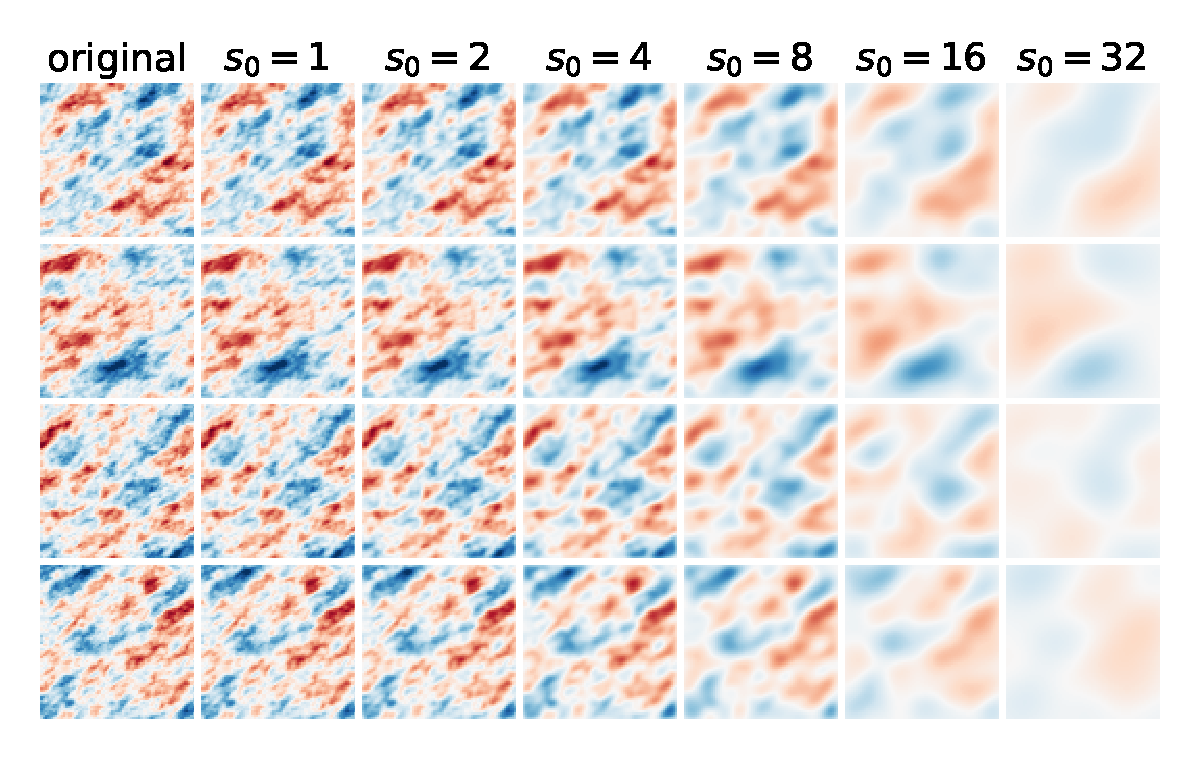
\includegraphics[width=\linewidth]{Figures/fake-seeing-nonp-thumbnails}\\
    (b)\\
    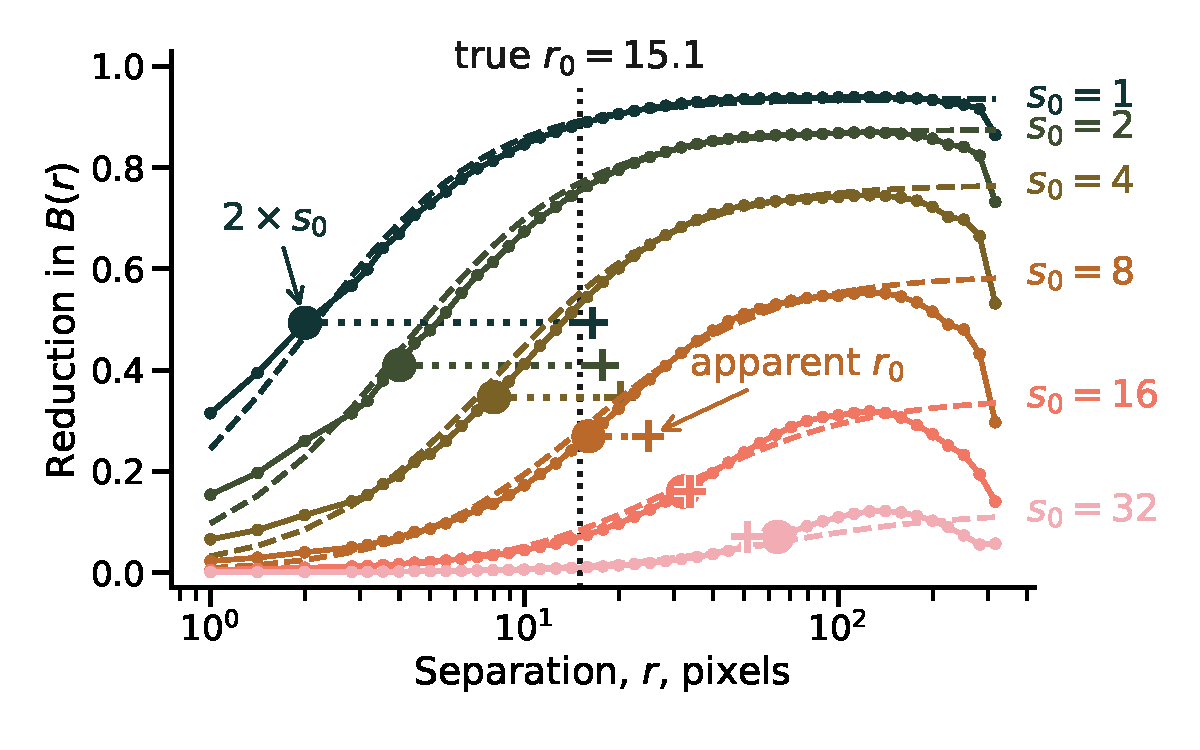
\includegraphics[width=\linewidth]{Figures/fake-seeing-nonp-reduction}
  \end{tabular}
  \caption{Effects of seeing on the structure function.
    (a)~Each row shows a different simulated random velocity field on a \(256^2\) grid
    (see text for details).
    The left column shows the original field,
    while the remaining columns show the effects of smoothing by a gaussian kernel
    with RMS width \(s_0\) from 1 to 32 pixels.
    The same color scale is used for all columns, ranging from \(-3\) to \(+3\) times
    the standard deviation of the unsmoothed map.
    (b)~Relative change in the second-order structure function due to the gaussian smoothing.
    Solid lines with symbols show the average over the 4 maps of
    \(B(r, s_0) / B(r, s_0 = 0)\) as a function of separation \(r\),
    with a separation of \(2 s_0\) indicated by a large filled circle on each curve.
    Dashed lines shows the empirical fit discussed in the text.
    The dotted line shows the correlation length of the original fields,
    while colored plus symbols show the apparent correlation length of the smoothed fields.
  }
  \label{fig:seeing-reduction}
\end{figure}

Ground-based astronomical observations are affected by the seeing produced by the atmosphere.
When calculating the structure function of the observational data, the seeing affects the structure function results at small-scale separations due to the smoothing of velocity fluctuations between adjacent pixels.
To study the effect of the seeing we calculate the structure function of simulated velocity maps where an artificial Gaussian seeing with different line widths has been introduced.
The artificial velocity maps are created in the same way as in Section~\ref{sec:finite-box-effects}.
The seeing in velocity maps is added via the \texttt{astropy} Python library \citep{astropy:2013} using the \textit{Gaussian2DKernel} command. 

Fig. \ref{fig:seeing-reduction}a shows column an artificial velocity field of 512 \(\times\) 512  divided into four maps of 256 \(\times \) 256 pixels each which are displayed in each row.
A Gaussian seeing \(s_0 \) is applied to each division with an RMS width given by \(s_0 = 2^n\) pixels with \(n = 0-5\) shown in the different columns. 
The structure function is computed in these maps and the averaged considering the same seeing. 

The solid lines in Figure \ref{fig:seeing-reduction}b show the ratio of the averaged structure function of the maps with their respective seeing to the unsmoothed map: \(B (r, s_0 ) / B (r, s_0 = 0) \).
The circle symbols indicate the value of 2\(s_0\), the plus symbols indicate the apparent correlation length of the smoothed maps and the vertical dotted line indicates the true \(r_{0}\). 

The dashed lines in Figure \ref{fig:seeing-reduction}b are  empirically fits for each ratio and characterizes the decrease in the structure function for each value of seeing.
To obtain this fit, we start from a convolution of an emission line and Gaussian seeing.
The emission line has the form \(\text {I}(x, v) = \text{I}_0 \phi [v; \overline {v} (x), \sigma_0]\) and has uniform width and brightness where the only change with respect to position is the velocity centroid.
The proposed seeing is \(\text{K}(x, s_0)\) of the form \(1 / \sqrt{2 \pi s_0} \exp^ {-x^ 2 / 2s_0 ^ 2} \).
The convolution \(\text{I}(x, v) \otimes \text{K}(x, s_0) \) is performed to obtain the smoothed map, \(\text {\~I} (x, v) \). 

Then we calculate the average velocity difference of the original map, \(\Delta v \), and the smoothed map, \(\tilde{\Delta v}\), in the arbitrary points \( x = \{0, \delta \} \).
The expansion of the convolution at small separations gives a term \(S_0(r; s_0)\) that modifies the structure function which has the form: 

\begin{equation}\label{eq:seeingcon}
S (r;s_0) = \tanh^2 \left[ \left( \dfrac{r}{2s_0} \right)^2 \right]
\end{equation}

Subsequently, the equation \ref{eq:seeingcon} is empirically modified and we obtain: 

%\begin{equation}\label{eq:seeingemp}
%S(r; s_0, r_0) =  \frac{e^\frac{-s_0}{r_0}}{2} \left(1 + \tanh{a \text{ln} \frac{r}{2s_0}} \right)
%\end{equation}
%
%and the final form of the equation \ref{eq:seeingemp} after a mathematical simplification gives: 

\begin{equation}\label{eq:seeingemp2}
S(r; s_0, r_0) = \frac{e^\frac{-s_0}{r_0}}{1+(\frac{2s_0}{r})^{2a}}
\end{equation}
%
which describes the dashed lines in Figure \ref{fig:seeing-reduction}b. 
The equation \ref{eq:seeingemp2} is used to correct the observational structure function in equation \eqref{eq:sf-functional}. 

\section{\boldmath Notes on individual \hii{} regions}
\label{sec:notes-individual-hii}
For each region or pair of regions in our sample,
we give a more detailed description of the physical properties
(supplementing section~\ref{sec:regions-milky-way})
together with additional details of the structure function
(supplementing section~\ref{sec:results})
and comparison with previous results from the literature
(supplementing section~\ref{sec:comp-with-prev}).

%the model fit to

\subsection{Orion Nebula}
\label{sec:orion-nebula}

The Orion Nebula (M42) is the prototype of a galactic HII region located at a distance of 440 pc \citetext{\SI{1}{\arcsecond} = \SI{0.002}{pc} ; \citealp{2008AJ....136.1566O}}.
The O7 V star \(\theta^{1}\) Ori C is the most luminous and hottest star \citep{2006A&A...448..351S} with an ionizing flux \(Q_0\) of  \SI{e49.12}{photons.s^{-1}}. 
With other 3 B-type stars they form the Trapezium cluster.
The bright region that surrounds these massive ionizing stars is called the the Huygens region.
%In the southwest direction of the Huygens region there is a drop in the brightness as one approach a much larger region called Extended Orion Nebula \citetext{EON henceforth;  \citealp{2008Sci...319..309G}}
The position of Orion near the side of the Orion Molecular Cloud (OMC-1) make it an ongoing star formation with a large population of young star, some of which are the sources of stellar jets and Herbig-Haro objects \citep{1993ApJ...410..696O}.
Its physical properties and kinematics, along its stellar population are documented in \citet{2001ARA&A..39...99O}.

\subsubsection{Observed structure function and model fit}
\label{sec:observ-struct-funct-orion}

Figure~\ref{fig:strucfunc-fit-Galactic}a shows the structure function of the Orion core.
In this case we merge the first three points of the structure function.
A detailed description of the model fit is given in
section~\ref{sec:example-results-orion} and will
not be repeated here.
At the largest scales, which are not used in the model fitting,
one sees a downturn in the structure function from
\SI{22}{km^{2}.s^{-2}} for \(r < \SI{0.3}{pc}\) to
\SI{7}{km^{2}.s^{-2}} at \(r  \SI{0.5}{pc}\)
(open symbols in Figure~\ref{fig:strucfunc-fit-Galactic}a).
This is similar to the behavior expected for tapered fluctuations
(see section~\ref{sec:limit-model-struct} and Figure~\ref{fig:model-strucfunc}b)
in which the velocity dispersion is higher in the center of the map
than in the periphery.

Figure~\ref{fig:strucfunc-fit-Galactic}b shows the structure function of the Extended Orion Nebula, which is ten times larger than the core in linear size,
but observed at a much lower angular resolution
(see Figures~\ref{fig:hii-regions} and~\ref{fig:velocity-maps}).
The data for this region are the lowest quality of all the regions in
our sample, and there are too many degeneracies between the parameters
to achieve a credible fit using the full model.
We therefore fix the power slope to \(m = 1\),
which implies that noise makes a significant contribution at all scales
in order to reproduce the observed flat structure function.
In turn, this implies that the true \(\sigma^2\pos = \SI{5}{km^2.s^{-2}}\),
which is lower than the \SI{7}{km^2.s^{-2}}
that would be naively derived from the observations
(compare green and orange lines in Figure~\ref{fig:strucfunc-fit-Galactic}b).

The seeing width is much smaller than the angular scale of the observations
\subsubsection{Comparison with previous studies}
\label{sec:comparison-orion}

\citet{arthur2016turbulence} carried out a complete analysis by calculating the structure function of different emission lines in the inner Orion Nebula.
They observed a tendency that higher ionization lines presents higher  dispersion and the steepness of the structure function slope. 
Their results just consider one Gaussian component. 
The power-law index obtained by \citet{arthur2016turbulence} are \(m \sim 1.2 \pm 0.1\) for \halpha\ and [OIII] emission lines and for [SII] they found \(m \sim 0.8 \pm 0.1\). 
The correlation length for all lines is \SI{\approx 0.05}{pc}, value obtained when the structure function is equal to \(\sigma\pos^2\).
For the same \halpha\ observation we obtained a value of \num{1.07} and a correlation length of \SI{0.068}{pc}. 
Although the work of \citet{arthur2016turbulence} follows a different methodology, the values of \(r_0\) and \(\sigma\pos^2\) fall within the margin of error of our own results.

\subsection{Lagoon Nebula}
\label{sec:lagoon-nebula}

The Lagoon Nebula (M8, NGC6523) is located at a distance of 1 250 pc \citetext{\SI{1}{\arcsecond} = \SI{0.006}{pc} ; \citealp{2005A&A...430..941P}}.
It has a luminosity in \ha{} of \SI{e37.47}{erg.s^{-1}} \citep{1984ApJ...287..116K}.
The mean non-thermal linewidth in \ha{} is \SI{11.7 \pm 1.6}{km.s^{-1}} \citep{1973ApJ...183..851B}.
It contains the young stellar cluster NGC6530 and the region is illuminated by different massive stars of spectral types O and B, the hottest being 9 Sgr, type O4V \citep{Damiani:2017b}.
Optically, the brightest part of the nebula is called 'Hourglass nebula' which surrounds and obscures the O7 star Herschel 36 \citep{1986AJ.....91..870W}. 
The velocity field shows several expanding shells, related to the stellar population, and the massive protostar M8East-IR \citep{1984ApJ...278..170S} indicating that recent star formation. 
A blueshifted, neutral layer is also in very good agreement with predictions of champagne-flow models of blister HII regions \citep{Damiani:2017b}. 
The properties of the nebula are reviewed by \citet{2008hsf2.book..533T}.

\subsubsection{Observed structure function and model fit}
\label{sec:observ-struct-funct-lagoon}

The Figure~\ref{fig:strucfunc-fit-Galactic}c shows the structure function of the Lagoon nebula.
%There aren't any points affected by the seeing which has a value of \SI{0.006}{pc} (\(s_0\)=\SI{1}{\arcsecond}).
In this case we merge the first two points.
The Lagoon nebula presents a non-uniform behavior below the correlation length but it is possible to see the characteristic ascending values of the structure function.
%The turbulent parameters that fits our model are a \(r_0\) of \SI{1}{pc}, a \(\sigma^2\pos\) of \SI{7}{km^{2}.s^{-2}} and an index of \num{1.17}.
At large scales there is an indication of some periodic behavior followed by ascending \(B(r)\) values at largest separation.
A value of\(B(r)\) of order 2\(\sigma^2\pos\) is \(\sim\)\SI{14}{km^{2}.s^{-2}} at a separation of \(\sim\)\SI{2.5}{pc}. 
Then there is a diminution at \SI{4.5}{pc} down to a value of \SI{11}{km^{2}.s^{-2}}.
From this point the structure function ascends until it reaches \SI{66}{km^{2}.s^{-2}} around \SI{20}{pc}.

\subsubsection{Comparison with previous studies}
\label{sec:comparison-lagoon}
The structure function of the Lagoon Nebula was previously
studied by \citet{Chakraborty:1999a} using the [\ion{O}{3}] \Wav{5007} line,
finding an approximate power law behavior (\(m = 0.46\))
on scales of \num{0.01} to \SI{0.2}{pc}.
No flattening of the structure function at the largest scales
was seen,
but that is to be expected due to the finite box effect
(see Appendix~\ref{sec:finite-box-effects})
given that we determine the correlation length to be \(r_0 \approx   \SI{1}{pc}\) for this nebula,
which is several times larger than the region mapped by \citet{Chakraborty:1999a}.
On the other hand, the magnitude of the velocity dispersion found by these authors greatly exceeds our own measurements.
For instance, they find \(B(r) = \SI{278}{km^2.s^{-2}}\) at \SI{0.2}{pc}, whereas we find \(B(r) \approx \SI{2}{km^2.s^{-2}}\) at the same scale, which corresponds to a discrepancy of more than a factor of a hundred in \(\sigma^2\pos\).
This may be due in part to the fact that \citet{Chakraborty:1999a}
observed a small and atypical part of the nebula known as the
Hourglass region, which includes a cluster of very young stars
\citep{Arias:2006e}. 
In the case of the Orion Nebula we found that the velocity dispersion
of the central region was larger than that of the extended nebula
and this could be an example of a similar phenomenon,
albeit to a more extreme degree.



\subsection{Carina Nebula}
\label{sec:carina-nebula}

The Carina nebula is a large star-forming complex located at a distance of 2 350 pc \citetext{\SI{1}{\arcsecond} = \SI{0.01}{pc} ; \citealp{2006ApJ...644.1151S}}.
Using the \ha{} luminosity as a diagnostic of the ionizing flux \(Q_0\) \citet{2007MNRAS.379.1279S} measured a value of \SI{e50.47}{photons.s^{-1}}.
Young clusters like Trumpler 14 and 16, and Collinder 228 form the Car OB1 association, one of the largest OB associations on the Galaxy.
This OB association has more than 65 stars earlier than B0, and several Wolf-Rayet (WR) stars.
The most luminous star is the blue variable $\eta$ Car.
As a star formation region, it presents several phenomena related with young stars as evaporating protoplanetary discs, erosion of large dust pillars and the triggering of a second generation of embedded stars and Herbig-Haro objects, to mention some \citetext{see \citealp{2008hsf2.book..138S} and reference therein}. 
This region can be consider as a bridge between the detailed star-formation regions like Orion, and much more distant regions like 30 Doradus.

\subsubsection{Observed structure function and model fit}
\label{sec:observ-struct-funct-carina}

(The Figure~\ref{fig:strucfunc-fit-Galactic}d shows the structure function of the Carina nebula.
%The seeing is \SI{0.008}{pc} (\(s_0\)=\SI{1.3}{\arcsecond}) and there are just a couple of points that lie below the true model, indicating that the majority of points isn't affected by the seeing.
For this region we merge the first two points of the structure function.
As the Lagoon nebula, Carina also shows a non-uniform behavior below the correlation length.
%The correlation length is \SI{0.56}{pc} pc at a \(\sigma^2\pos\) of \SI{18}{km^{2}.s^{-2}} and an index of \num{1.14}.
At larges scales the structure function of the Carina nebula follows a pattern that resembles the homogeneous fluctuation of Figure~\ref{fig:model-strucfunc}a.
The structure function reaches a plateau around \SI{36}{km^{2}.s^{-2}} at \(\sim\) \SI{2}{pc}.
When \(r >\)\SI{6}{pc} the structure functions shows a small amplitude periodic pattern around 2\(\sigma^2\pos\).


\subsubsection{Comparison with previous studies}
\label{sec:comparison-carina}

We have found no previous studies of Carina's structure function in the literature.

\subsection{30 Doradus}
\label{sec:30-doradus}

The 30 Doradus (Tarantula Nebula) nebula is located at a distance of \SI{49.9}{kpc} \citetext{\SI{1}{\arcsecond} = \SI{0.24}{pc} ; \citealp{2013Natur.495...76P}}.
It is a luminous star-forming region in the LMC (Large Magellanic Cloud) and is the most luminous complex in the Local Group \citep{1984ApJ...287..116K}.
The central ionized region spans for \SI{40}{pc} and host the massive, dense star cluster R136 %\citep{1991IAUS..148..145W}. %Note: check the bibliographic format
The ionizing output \(Q_0\) of R136 is \SI{e51.4}{photons.s^{-1}} \citep{2020MNRAS.499.1918B}.
The mean non-thermal linewidth in \ha{} is \SI{22}{km.s^{-1}} \citep{2013A&A...555A..60T}.
It host the active star forming region NGC 2070 \citep{2013AJ....145...98W} where the star-formation rate has recently peaked \citep{2015ApJ...811...76C}. 
NGC 2070 host a population of OB and WR stars \citep{2011A&A...530A.108E}.
This nebula is commonly used as a comparison for extragalactic star-forming regions.

\subsubsection{Observed structure function and model fit}
\label{sec:observ-struct-funct-30dor}

The 30 Doradus structure function is shown in Figure~\ref{fig:strucfunc-fit-MC}a.
In this case we merge the first five points of the structure function.
%The seeing value for this regions is \SI{0.16}{pc} (\(s_0\)=\SI{0.7}{\arcsecond}) and just one %point of the structure function is below this value.
%Until a separation of \SI{1.7}{pc} is reached, the structure function lies below the true model.
%The correlation length is \SI{4}{pc} at a \(\sigma^2\pos\) of \SI{297 \pm 9}{km^{2}.s^{-2}} and an index of \num{0.85}.
At large separations 30 Doradus structure function presents a behavior of tapered fluctuations. The maximum \(B(r)\) value is \SI{655}{km^{2}.s^{-2}} at a separation of \SI{21}{pc}. 
From there \(B(r)\) values descends until they reach \SI{250}{km^{2}.s^{-2}} at \SI{38}{pc}.

\subsubsection{Comparison with previous studies}
\label{sec:comparison-30dor}

The first attempt at characterizing turbulence in a giant extragalactic HII region, GEHR, was done by \citet{1961MNRAS.122....1F} with the 30~Doradus complex, finding no indication of turbulent motions between scale of \num{10} and \SI{100}{pc}.
\citet{Melnick:2021x} also investigated the structure function in 30 Doradus finding on their results that the structure function is entirely flat on scales from \num{3} to \SI{200}{pc}.
The above does not coincide with our results, since we establish the existence of correlations up to the maximum value of the structure function that occurs at \SI{20}{pc}, separation where a value of 2\(\sigma\pos^2\) is reached.
The VLT FLAMES/GIRAFFE observations of \citet{Melnick:2021x} may not have had the resolution to resolve the correlations at small separations, however an inspection of its velocity map (figure 7 in their work) shows that the velocity distribution it is far from completely random.
This is the first time turbulence is characterized in 30~Doradus using the structure function.


\subsection{NGC 346}
\label{sec:ngc-346}

NGC 346 is the most active star-formation region in the SMC (Small Magellanic Cloud) located at a distance of 62 kpc \citetext{\SI{1}{\arcsecond} = \SI{0.30}{pc} ; \citealp{2001ApJ...562..303D}}. 
It has more than 30 O stars that ionize N66, the largest HII region \citep{2011ApJ...740...10D}.
N66 has an \ha{} luminosity of \SI{e38.77}{erg.s^{-1}}, almost 60 times higher compared to the Orion Nebula \citep{2010A&A...517A..39H,1984ApJ...287..116K}.
\citet{2008ApJ...688.1050G} propose an expanding HII region or bubble blown by the winds of the massive progenitor as a mechanism that shapes the recent star formation in this region, in addition to the photoionizing process of the OB stars. 
This mechanism is similar to shell-like HII regions, with a central cluster in a cavity, and with ongoing star formation triggered around their periphery.
Using a Gaussian single-component \citet{2003ApJ...586.1179D} find a corrected FWHM bulk turbulence of \SI{23.8}{km.s^{-1}}. 

\subsubsection{Observed structure function and model fit}
\label{sec:observ-struct-funct-346}

The Figure~\ref{fig:strucfunc-fit-MC}b shows the structure function of NGC 346.
%In this case we merge the first three points of the structure function.
%The seeing value is \SI{0.07}{pc} (\(s_0\)=\SI{0.23}{\arcsecond}).
For this region the first ten points lie below the true model.
At separations above \SI{0.4}{pc} the observed structure functions is coincident with the true model. 
%The correlation length is \SI{2}{pc} at a \(\sigma^2\pos\) of \SI{35}{km^{2}.s^{-2}} and an index of \num{0.80}.
For scales above \SI{12}{pc} and a \(B(r)\) value of \SI{65}{km^{2}.s^{-2}} the structure function shows a pattern of ascending values until it reaches \SI{146}{km^{2}.s^{-2}} at \SI{24}{pc}.

\subsubsection{Comparison with previous studies}
\label{sec:comparison-346}

We have found no previous studies of NGC~346's structure function in the literature.

\subsection{Hubble X and Hubble V in NGC 6822}
\label{sec:6822-hubble}
%
The irregular dwarf galaxy, NGC 6822, is located at a distance of 500 kpc \citetext{\SI{1}{\arcsecond} = \SI{2.42}{pc} ; \citealp{2012A&A...540A.135S}} and the brightest HII regions are Hubble X and Hubble V (HX and HV hereafter). %(1'' = 2.4 pc)
Luminosity \ha{} for HV is \SI{e38.3}{erg.s^{-1}} and for HX is \SI{e38.21}{erg.s^{-1}} \citep{2002MNRAS.329..481B}.
The mean non-thermal linewidth in \ha{} is \SI{10.5 \pm 0.02}{km.s^{-1}} for HX and \SI{10.3 \pm 0.03}{km.s^{-1}} \citep{1986A&A...160..374H}.
Two recognized OB associations are identified within these HII regions \citep{1991ApJ...379..621H,1992AJ....104.1374W}.
HV is located near 'Hodge OB 8' and HX is located near 'Hodge OB13'  \citep{1999PASP..111.1382O}.
\citet{1993PASJ...45..693T} realize a study on the kinematics of HX and HV. 

\subsubsection{Observed structure function and model fit}
\label{sec:observ-struct-funct-hubbles}

In the Figure~\ref{fig:strucfunc-fit-ExtraGal}a we show the structure function of Hubble V.
For the observations coming from the TAURUS-II instrument there wasn't any merging of points at small scales.
%The value of the seeing for this regions is \SI{0.5}{pc} (\(s_0\)=\SI{0.2}{\arcsecond}).
%All the structure function points lies below the true model.
%The correlation length is \SI{3.5}{pc} at a \(\sigma^2\pos\) of  \SI{10}{km^{2}.s^{-2}} and an index of \num{0.75}.
The maximum \(B(r)\) value is \SI{18}{km^{2}.s^{-2}} at a separation of \SI{25}{pc}. 
From there \(B(r)\) values descends until it reaches \SI{14}{km^{2}.s^{-2}} at \SI{45}{pc}, then it rises for the next point at \SI{50}{pc} with a value of \SI{15}{km^{2}.s^{-2}}.
Finally the structure functions descends at \SI{9}{km^{2}.s^{-2}} for a separation of \SI{70}{pc}.

The Hubble X structure function is shown in Figure~\ref{fig:strucfunc-fit-ExtraGal}b.
%The seeing is \SI{0.6}{pc} (\(s_0\)=\SI{0.24}{\arcsecond}) and as in Hubble V the observed structure function lies below the true model.
%The correlation length is \SI{4}{pc} at a \(\sigma^2\pos\) of \SI{15}{km^{2}.s^{-2}} and an index of \num{0.93}.
A plateau is reached around \SI{25}{km^{2}.s^{-2}} at a separation of \SI{14}{pc} and a maximum \(B(r)\) value of \SI{31}{km^{2}.s^{-2}} at a separation of \SI{36}{pc}.

\subsubsection{Comparison with previous studies}
\label{sec:comparison-carina}

We have found no previous studies of the structure functions
of Hubble~V or~X in the literature.

\subsection{NGC~595 and NGC~604 in M33}
\label{sec:m33-ngc}

M33 is the third largest galaxy in the Local Group located at the distance of 840 kpc \citetext{\SI{1}{\arcsecond} = \SI{4.07}{pc} ; \citealp{2015KamKinematics}} and is of morphological type SA(s)cd.
The two brightest HII regions in the galaxy are NGC 604 and NGC 595.

NGC 604 is the second brightest \hii{} region in the Local Group after 30~Dor in the Large Magellanic Cloud and is forty times larger ($\sim $ 400 pc) and 6,000 times brighter than Orion in our Milky Way galaxy.
It is the brightest giant \hii{} region in the M33 galaxy and is visually dominated by a big loop, big shells and different size filaments.
It has a luminosity in \ha{} of \SI{e39.42}{erg.s^{-1}} \citep{2002MNRAS.329..481B}.
The mean non-thermal linewidth in \ha{} is \SI{17.8 \pm 0.3}{km.s^{-1}} \citep{1986A&A...160..374H}.
Using photometry from the HST \citet{1996ApJ...456..174H} identified that the stars are separated into a primary cluster within NGC 604, and a secondary to the north of the region.
In the primary there are \(\sim\)200 OB stars, candidate to red supergiants (RSGs) and the presence of WR stars.
For the northern cluster they find eight luminous stars and no evolved massive stars.
More Recently, \citet{2011MNRAS.411..235E} studied 10 WR stars and propose at least 4 RSGs candidates.
\citet{2012AJ....143...43F} focused on the massive young stellar objects (MYSOs).
The average ages for the stars, was determined to be from  \num{3} to \SI{5}{Myr} \citep{1996ApJ...456..174H} and with the RSGs as an older population have an age of 12.4\(\pm\)2.1 Myr \citep{2011MNRAS.411..235E}.
This suggest that two episodes of star formation, at least, have taken place in the GEHR.

% and in L$_{X}$=9.3$\times$ 10$^{35}$ erg s$^{-1}$ \citep{2008ApJ...685..919T}.
%\citet{2012ApJ...761....3M} derive an average age of 4$\pm$1 Myr and a total stellar mass of 1.6$^{+1.6}_{-1.0} \times$ 10$^{5}$M$_{\odot}$ for the region.

NGC 595 is the second brightest giant HII region in the M33 galaxy and has an \ha{} shell morphology that is related to the stellar winds of the several massive stars located in its interior.
It has a luminosity in \ha{} of \SI{e38.95}{erg.s^{-1}}\citep{2002MNRAS.329..481B}.
The mean non-thermal linewidth in \ha{} is \SI{16.8 \pm 0.1}{km.s^{-1}} \citep{lagrois2009multi}.
\citet{1993AJ....105.1400D} use optical photometry to propose 11 WR stars. 
Using HST/WFPC-2 images \citet{1996AJ....111.1128M} found approximately 250 stars of the OB type, 13 Supergiants and 10 WR, confirming previous candidates.
They derived and age of 4.5\(\pm\)1.0 Myr consistent with \citet{1993AJ....105.1400D}.
\citet{2010MNRAS.402.1635R} used Integral Field Spectroscopy (IFS) to present a resolved study of the physical properties of the ionized gas and the ionized structure.
They also confirm the presence of previous cataloged WR stars and detect new candidates, and propose classical emission-line ratios as metallicity calibrators.
\citet{lagrois2011} present a kinematic study of the regions using optical emission lines and and radio 21 cm line observations.
They proposed Champagne flows at the periphery of the molecular cloud leading to accelerated ionized material.

\subsubsection{Observed structure function and model fit}
\label{sec:observ-struct-funct-m33}

In the Figure~\ref{fig:strucfunc-fit-ExtraGal}c we show the structure function of NGC 595.
%The seeing is \SI{0.3}{pc} (\(s_0\)=\SI{0.1}{\arcsecond}) and for this region only the first two points are below the true model. 
%The correlation length is \SI{12}{pc} at a \(\sigma^2\pos\) of \SI{54}{km^{2}.s^{-2}} and an index of \num{1.3}.
At large scales the structure function behaves following the tapered fluctuations pattern.
A maximum \(B(r)\) value of \SI{104}{km^{2}.s^{-2}} is reached at \SI{33}{pc}. 
From there the structure functions decays following a scatter pattern until it reaches \SI{54}{km^{2}.s^{-2}} at a separation of \SI{211}{pc}.

In the Figure~\ref{fig:strucfunc-fit-ExtraGal}d we show the structure function of NGC 604.
%The seeing is \SI{1.7}{pc} (\(s_0\)=\SI{0.42}{\arcsecond}) and the structure function of this region lies below the true model for most of the separation range.
%The correlation length is \SI{10}{pc} at a \(\sigma^2\pos\) of \SI{71}{km^{2}.s^{-2}} and has an index of \num{1}.
The structure function present clear characteristics of periodic oscillations at large scales.
A periodic pattern for the structure function appears with a maximum \(B(r)\) value of \SI{143}{km^{2}.s^{-2}} that is reached at \SI{60}{pc}, then the oscillation cause a minimum of \SI{54}{km^{2}.s^{-2}} at \SI{133}{pc} and finally it goes back up again at \SI{211}{pc} to a \(B(r)\) value of \SI{123}{km^{2}.s^{-2}}.

\subsubsection{Comparison with previous studies}
\label{sec:comparison-m33}

For NGC 604 there is good agreement in our structure function results and previous studies because where are using the same TAURUS-II data as \citet{Melnick:2021x} and \citet{Medina-Tanco:1997a}.
Despite this general agreement the interpretations in each study is different.
\citet{Medina-Tanco:1997a} conclude about a double regime acting on the kinetic energy spectrum.
According to this double cascade, turbulence is being forced at scales of \(\approx\) \SI{10}{pc} while and energy cascade has developed down to the smallest scales and other, as an inverse cascade, extends up to scale of \(\approx\) \SI{70}{pc}.
\citet{Medina-Tanco:1997a} mentioned different characteristic scale lengths, the most notorious is the \SI{\sim 10}{pc}, and they interpret it as possible source on energy associated with the expansion of shocks coming from wind bubbles.  
\citet{Melnick:2021x} addresses some issues with TAURUS II data while comparing profiles between the previous instrument TAURUS I where there exist a difference between observations (see section 4.1 on their paper).
They mentioned that one problem with \citet{Medina-Tanco:1997a} structure function is that they didn't take into account the observational seeing.
This would invalidate they results and \citet{Melnick:2021x} consider that taking out the structure function values that fall within this range would make the structure function flat at scales \(<\)\SI{10}{pc}, so they rule out \citet{Medina-Tanco:1997a} results.
Finally they point out, and we agree, the importance of observing NGC 604 at higher spatial resolution. 
Our Fig. \ref{fig:strucfunc-fit-ExtraGal}d shows in fact that there is a velocity structure in NGC 604. 
None of the previous studies obtained a power-law index or correlation length for the structure function to compare our results.

For our NGC 595 \halpha\ emission line results there is no correspondence in the structure function from the previous investigations of \citet{lagrois2009multi} and \citet{lagrois2011}.
Our observations cover the brightest part of the region and have smaller resolution than theirs.
As a consequence \citet{lagrois2009multi} and \citet{lagrois2011} structure functions results does not cover scales $<$10 pc, where in our results the correlation is taking place.
One big difference is that \citet{lagrois2011} apply a  filter to the velocity field to get rid of non-turbulent movements.
As a comparison for the filtered turbulent parameters they present a correlation length of \SI{43}{pc} and the power-law index they provide is \num{1.55 \pm 0.01}.
Other difference in their methodology is that they use the normalized structure function value of 2\(\sigma\pos\) to obtain the correlation length.
%Using their unfiltered data the correlation length is \(\sim\) \SI{90}{pc} and using the same criteria as our it is \(\sim\) \SI{40}{pc} and the slope would be shallower. 
Their velocity centroid \(\sigma\) is \SI{5.92 \pm 0.15}{km.s^{-1}} while we have \SI{7.3\pm 2}{km. s^{-1}} which fall within the uncertainties.
Due to the different observations and methodologies a direct comparison between structure functions is not possible.

\section{Additional covariance corner plots for model fits}
\label{sec:addit-covar-corn}
Supplementary online-only material.
%\clearpage

\begin{figure*}
  \centering
  \sfcfigggg{OrionS}{OrionLH}{M8}{CarC}
  \caption{
    Corner plots of covariances between
    fitted model parameters
    of \ha{} structure function
    for Galactic \hii{} regions.
  }
  \label{fig:corner-Galactic}
\end{figure*}


\begin{figure*}
  \centering
  \sfcfigg{N346}{Dor}
  \caption{
    Same as figure~\ref{fig:corner-Galactic}
    except for Magellanic Cloud \hii{} regions. 
  }
  \label{fig:corner-MC}
\end{figure*}

\begin{figure*}
  \centering
  \sfcfigggg{HV}{HX}{N595}{N604H}
  \caption{
    Same as figure~\ref{fig:corner-Galactic}
    except for \hii{} regions in more distant
    Local Group Galaxies.
  }
  \label{fig:corner-ExtraGal}
\end{figure*}

\begin{table*}
\begin{center}\caption{Fitting parameters.}
\begin{tabular}{cCCCCCCCC}\toprule
\hii{}    &  \text{No. points} & \text{Relatively}  & \text{Weight / No. points}     &  \text{Weight / No. points}     & \text{Max.}  & \text{Reduced} & \text{Autocorrelation } & \text{Acceptance}\\
Region    &  \text{merged} & \text{uncertainty} & \text{Small scales} &  \text{Large scales} & \text{separation}  & \text{chi-square} & \text{time} & \text{fraction}\\
\midrule
Orion     & 3 & 0.02    &  -           &   -        & 0.5L  & 0.82 & 60  & 0.55\\
EON       & - & 0.03   &  2.0 / 3     &   3.0 / 3        & 0.7L  & 0.62 & 40 & 0.64\\
Lagoon    & 2 & 0.08    &  2.5 / 16    &   2.5 / 8  & 0.5L  & 0.94 & 72  & 0.50\\
Carina    & 2 & 0.055   &  3.0 / 14    &   3.0 / 4  & 0.5L  & 0.94 & 72  & 0.50\\
30 Dor    & 5 &  0.07   &  -           &   -        & 0.9L  & 0.98 & 84  & 0.54\\
NGC 346   & 3 & 0.02    &  -           &   -        & 0.5L  & 0.83 & 64  & 0.54\\
Hubble V  & - & 0.05    &  2.0 / 3     &   -        & 0.6L  & 0.86 & 340 & 0.44\\
Hubble X  & - & 0.032   &  2.0 / 4     &   2.0 / 6  & 0.5L  & 0.73 & 79  & 0.49\\
NGC 595   & - &  0.055  &  4.5 / 3     &   3.0 / 5  & 0.5L  & 0.83 & 67  & 0.51\\
NGC 604   & - &  0.08  &   2.0 / 3    &   1.5 / 2 & 0.5L  & 0.92 & 112 & 0.45\\
\bottomrule
\end{tabular}\label{tab:fitting-parameters}
\end{center}
\end{table*} 

%%%%%%%%%%%%%%%%%%%%%%%%%%%%%%%%%%%%%%%%%%%%%%%%%%
%%%%%%%%%%%%%%%%%%%%% END %%%%%%%%%%%%%%%%%%%%%%%%
%%%%%%%%%%%%%%%%%%%%%%%%%%%%%%%%%%%%%%%%%%%%%%%%%%
\clearpage
% Don't change these lines
\bsp	% typesetting comment
\label{lastpage}
\end{document}

% End of mnras_template.tex
%%% Local Variables:
%%% mode: latex
%%% TeX-master: t
%%% End:
